%https://github.com/SublimeText/LaTeXTools/issues/1439
%!TEX output_directory=latexcache

% You can build this using the command:
% latexmk -pdf -jobname=output -output-directory=cache -aux-directory=cache -pdflatex="pdflatex -interaction=nonstopmode" -use-make main.tex

% When the bibliography includes a cyclic reference to another bibliography,
% you need to run `pdflatex` 5 times on the following order:
% 1. `pdflatex`,
% 2. `biber`,
% 3. `pdflatex`
% 4. `pdflatex`
% 5. `pdflatex`
% 6. `biber`
% 7. `pdflatex`

% Monograph LaTeX Template for UFSC based on:
% 1. https://github.com/royertiago/tcc
% 2. http://portal.bu.ufsc.br/normalizacao/
% 3. https://github.com/evandrocoan/ufscthesisx
% 4. http://www.latextemplates.com/template/simple-sectioned-essay

% Initially translated from Portuguese with help of https://github.com/omegat-org/omegat <Computer Assisted Translation of LaTeX document>
% https://tex.stackexchange.com/questions/313732/computer-assisted-translation-of-latex-document

% Allows you to write your thesis both in English and Portuguese
% https://tex.stackexchange.com/questions/5076/is-it-possible-to-keep-my-translation-together-with-original-text
\newif\ifenglish\englishfalse
\newif\ifadvisor\advisorfalse

% Uncomment the line `\englishtrue` to set the document default language to English
% \englishtrue
\advisortrue

% https://tex.stackexchange.com/questions/131002/how-to-expand-ifthenelse-so-that-it-can-be-used-in-parshape
\newcommand{\lang}[2]{\ifenglish#1\else#2\fi}
\newcommand{\advisor}[2]{\ifadvisor#1\else#2\fi}

% https://tex.stackexchange.com/questions/385895/how-to-make-passoptionstopackage-add-the-option-as-the-last
% https://tex.stackexchange.com/questions/484400/changing-the-cleveref-package-language-conjunction-definition
% https://tex.stackexchange.com/questions/516058/why-isnt-my-biblatex-language-changing-when-passing-the-language-on-my-document
\ifenglish
    \PassOptionsToPackage{brazil,main=english,spanish,french}{babel}
\else
    \PassOptionsToPackage{main=brazil,english,spanish,french}{babel}
\fi

% Simple alias for English and Portuguese words
% https://tex.stackexchange.com/questions/513019/argument-of-bbltempd-has-an-extra
\newcommand{\brazilword}[1]{\protect\foreignlanguage{brazil}{#1}}
\newcommand{\englishword}[1]{\protect\foreignlanguage{english}{#1}}

% Allow you to write `Evandro's house` in latex as `Evandro\s house` instead of `Evandro\textquotesingle{}s house`
% https://tex.stackexchange.com/questions/31091/space-after-latex-commands
\newcommand{\s}[0]{\textquotesingle{}s\xspace}
\newcommand{\q}[0]{\textquotesingle{}\xspace}

% Uncomment the following line if you want to use other biblatex settings
% \PassOptionsToPackage{style=numeric,repeatfields=true,backend=biber,backref=true,citecounter=true}{biblatex}
\documentclass[
\lang{english}{brazilian,brazil}, % https://tex.stackexchange.com/questions/484400/changing-the-cleveref-package-language-conjunction-definition
12pt, % Padrão UFSC para versão final
a4paper, % Padrão UFSC para versão final
oneside, % Impressão nos dois lados da folha
chapter=TITLE, % Título de capítulos em caixa alta
section=TITLE, % Título de seções em caixa alta
]{setup/ufscthesisx}

% Utilize o arquivo aftertext/references.bib para incluir sua bibliografia.
% http://tug.ctan.org/tex-archive/macros/latex/contrib/cleveref/cleveref.pdf
\addbibresource{aftertext/references.bib}

% https://www.overleaf.com/learn/latex/Inserting_Images
\graphicspath{{pictures/}}

% FIXME: Preencha com seus dados
\autor{\brazilword{Raquel Cristina Schaly Behrens}}
\titulo{\lang{Expert Bee: An Expert System for Supporting Integrated Learning with Moodle and Beecrowd\protect}{Expert Bee: Um Sistema Especialista de Apoio à Aprendizagem Integrada ao Moodle e Beecrowd\protect}}

% FIXME: Se houver subtítulo, descomente a linha abaixo
%\subtitulo{\lang{Subtitle}{Subtítulo}}

% FIXME: Siglas para grau de formação Dr./Dra., Me./Ma, Bel. Bela. (inglês: PhD., MSc., Bs.)
\orientador[\lang{Supervisor}{Orientador(a)}]{\brazilword{Prof. Maicon Rafael Zatelli}, \lang{Phd.}{Dr.}}

% FIXME: Se houver coorientador, descomente a linha abaixo
\coorientador[\lang{Co-supervisor}{Coorientador(a)}]{\brazilword{Prof. Antonio Carlos Mariani}}

% FIXME: Preencher com o nome do Coordenador de TCCs/Teses do seu curso
\coordenador[\lang{Coordinator}{Coordenador(a)}]{\brazilword{Profa. Lúcia Helena Martins Pacheco}, \lang{Phd.}{Dra.}}

% FIXME: Local da sua defesa
\local{\brazilword{Florianópolis, Santa Catarina} -- \lang{Brazil}{Brasil}}

% FIXME: Ano da sua defesa
\ano{2024}
\biblioteca{\lang{University Library}{Biblioteca Universitária}}

% FIXME: Sigla da sua instituição
\instituicaosigla{UFSC}
\instituicao{\brazilword{Universidade Federal de Santa Catarina}}

% FIXME: Preencha com Tese, Dissertação, Monografia ou Trabalho de Conclusão de Curso, Bachelor's Thesis, etc
\tipotrabalho{\lang{Bachelor\s Thesis}{Trabalho de Conclusão de Curso}}

% FIXME: Se houver Área de Concentração, descomente a linha abaixo
% \area{\lang{Formal Languages}{Linguagens Formais}}

% FIXME: Preencha com Doutor, Bacharel ou Mestrando
\formacao{\lang
    {Bachelor of Science degree in Computer Science}
    {Bacharela em Ciência da Computação}%
}
\programa{\lang
    {Undergraduate Program in Computer Science}
    {Programa de Graduação em Ciência da Computação}%
}

% FIXME: Preencha com Departamento de XXXXXX, Centro de XXXXXX
\centro{\lang
    {INE -- Department of Informatics and Statistics, CTC -- Technological Center}
    {INE -- Departamento de Informática e Estatística, CTC -- Centro Tecnológico}%
}

% FIXME: Preencha com Campus XXXXXX     ou     Centro de XXXXXX
\campus{\brazilword{Campus Reitor João David Ferreira Lima}}

% FIXME: Data da sua defesa
\data{\lang{28 of november of}{28 de novembro de} 2024}

% O preambulo deve conter tipo do trabalho, objetivo, nome da instituição e a área de concentração.
\preambulo{\lang%
    {%
        \imprimirtipotrabalho~submitted to the \imprimirprograma~of
        \imprimirinstituicao~for degree acquirement in \imprimirformacao.%
    }{%
        \imprimirtipotrabalho~submetido ao \imprimirprograma~da
        \imprimirinstituicao~para a obtenção do Grau de \imprimirformacao.%
    }%
}

% Allows you to use ~= instead of `\hyp{}`
% https://tex.stackexchange.com/questions/488008/how-to-create-an-alternative-to-shortcut-or-hyp
% https://tex.stackexchange.com/questions/405718/depending-on-babel-language-setting-i-get-biblatex-error-argument-of-language
% https://tex.stackexchange.com/questions/340661/argument-of-languageactivearg-has-an-extra-i-use-includegraphics-and-r
\useshorthands{~}\defineshorthand{~=}{\hyp{}}

\palavraschaveufsc{palavraschaveingles}   {beecrowd}
\palavraschaveufsc{palavraschaveportugues}{beecrowd}

\palavraschaveufsc{palavraschaveingles}   {moodle}
\palavraschaveufsc{palavraschaveportugues}{moodle}

\palavraschaveufsc{palavraschaveingles}   {expert system}
\palavraschaveufsc{palavraschaveportugues}{sistema especialista}

\palavraschaveufsc{palavraschaveingles}   {prolog}
\palavraschaveufsc{palavraschaveportugues}{prolog}

\palavraschaveufsc{palavraschaveingles}   {swi-prolog}
\palavraschaveufsc{palavraschaveportugues}{swi-prolog}

\palavraschaveufsc{palavraschaveingles}   {LTI}
\palavraschaveufsc{palavraschaveportugues}{LTI}

\palavraschaveufsc{palavraschaveingles}   {API}
\palavraschaveufsc{palavraschaveportugues}{API}

\palavraschaveufsc{palavraschaveingles}   {programming}
\palavraschaveufsc{palavraschaveportugues}{programação}


\hypersetup
{
    pdfsubject={Thesis' Abstract},
    pdfcreator={LaTeX with abnTeX2 for UFSC},
    pdftitle={\imprimirtitulo},
    pdfauthor={\imprimirautor},
    pdfkeywords={\lang{\palavraschaveinglessemitem}{\palavraschaveportuguessemitem}},
}

% Altere o arquivo 'settings.tex' para incluir customizações de aparência da sua tese
%----------------------------------------------------------------------------------------
%   Thesis Tweaks and Utilities
%----------------------------------------------------------------------------------------
\makeatletter


% Uncomment this if you are debugging pages' badness Underfull & Overflow
% https://tex.stackexchange.com/questions/115908/geometry-showframe-landscape
% https://tex.stackexchange.com/questions/387077/what-is-the-difference-between-usepackageshowframe-and-usepackageshowframe
% https://tex.stackexchange.com/questions/387257/how-to-do-the-memoir-headings-fix-but-not-have-my-text-going-over-the-page-botto
% https://tex.stackexchange.com/questions/14508/print-page-margins-of-a-document
% \usepackage[showframe,pass]{geometry}

% To use the font Times New Roman, instead of the default LaTeX font
% more up-to-date than '\usepackage{mathptmx}'
% \usepackage{newtxtext}
% \usepackage{newtxmath}

% https://tex.stackexchange.com/questions/182569/how-to-manually-set-where-a-word-is-split
\hyphenation{Ge-la-im}
\hyphenation{Cis-la-ghi}

% Add missing translations for Portuguese
% https://tex.stackexchange.com/questions/8564/what-is-the-right-way-to-redefine-macros-defined-by-babel
\@ifpackageloaded{babel}{\@ifpackagewith{babel}{brazil}{\addto\captionsbrazil{%
  \renewcommand{\mytextpreliminarylistname}{Breve Sumário}
}}{}}{}
\@ifundefined{advisor}{\newcommand{\advisor}[2]{#1}}{}

% Selects a sans serif font family
% \renewcommand{\sfdefault}{cmss}

% Selects a monospaced (“typewriter”) font family
% \renewcommand{\ttdefault}{cmtt}

% Spacing between lines and paragraphs
% https://tex.stackexchange.com/questions/70212/ifpackageloaded-question
\@ifclassloaded{memoir}
{
  % New custom chapter style VZ14, see other chapters styles in:
  % http://repositorios.cpai.unb.br/ctan/info/latex-samples/MemoirChapStyles/MemoirChapStyles.pdf
  \newcommand\thickhrulefill{\leavevmode \leaders \hrule height 1ex \hfill \kern \z@}
  \makechapterstyle{VZ14} { %
    % \thispagestyle{empty}
    \setlength\beforechapskip{50pt}
    \setlength\midchapskip{20pt}
    \setlength\afterchapskip{20pt}
    \renewcommand\chapternamenum{}
    \renewcommand\printchaptername{}
    \renewcommand\chapnamefont{\Huge\scshape}
    \renewcommand\printchapternum {%
      \chapnamefont\null\thickhrulefill\quad
      \@chapapp\space\thechapter\quad\thickhrulefill
    }
    \renewcommand\printchapternonum {%
      \par\thickhrulefill\par\vskip\midchapskip
      \hrule\vskip\midchapskip
    }
    \renewcommand\chaptitlefont{\huge\scshape\centering}
    \renewcommand\afterchapternum {%
      \par\nobreak\vskip\midchapskip\hrule\vskip\midchapskip
    }
    \renewcommand\afterchaptertitle {%
      \par\vskip\midchapskip\hrule\nobreak\vskip\afterchapskip
    }
  }

  % Apply the style `VZ14` just created
  % \chapterstyle{VZ14}

  % http://mirrors.ibiblio.org/CTAN/macros/latex/contrib/memoir/memman.pdf
  \setlength\beforechapskip{0pt}
  \setlength\midchapskip{15pt}
  \setlength\afterchapskip{15pt}

  % Memoir: Warnings “The material used in the headers is too large” w/ accented titles
  % https://tex.stackexchange.com/questions/387293/how-to-change-the-page-layout-with-memoir
  \setheadfoot{30.0pt}{\footskip}
  \checkandfixthelayout
}{}

% Controlling the spacing between one paragraph and another
% Default value for UFSC 0.0cm
\setlength{\parskip}{\advisor{0.0cm}{0.2cm}}

% Paragraph size is given by
% Default value for UFSC 1.5cm
% \setlength{\parindent}{1.3cm}

% https://tex.stackexchange.com/questions/148647/how-to-remove-space-before-enumerate
% https://tex.stackexchange.com/questions/433543/behaviour-of-enumitem-setlist
\advisor{}{
    \setlist*[enumerate]{label=\arabic*,}
    \setlist*[enumerateoptional]{label=\arabic*,}

    % https://tex.stackexchange.com/questions/24454/space-after-float-with-h
    % https://tex.stackexchange.com/questions/23313/how-can-i-reduce-padding-after-figure
    \AtBeginEnvironment{figure}{
      \setlength{\intextsep}{5pt} % Vertical space above & below [h] floats
      % \setlength{\textfloatsep}{10pt} % Vertical space below (above) [t] ([b]) floats
      % \setlength{\abovecaptionskip}{10pt}
      % \setlength{\belowcaptionskip}{5pt}
    }

    % Patch the `abntex2` citacao environment removing the extra space from its top
    % https://tex.stackexchange.com/questions/300340/topsep-itemsep-partopsep-and-parsep-what-does-each-of-them-mean-and-wha
    \xpatchcmd{\citacao}
    {\list{}}
    {\list{}{\topsep=0pt}}
    {}
    {\FAILEDPATCHINGCITACAO}
}


% Color settings across the document
\@ifpackageloaded{xcolor}
{
  % RGB colors in absolute values from 0 to 255 by using `RGB` tag
  \definecolor{darkblue}{RGB}{26,13,178}

  % Colors names definitions as RGB colors in percentage notation by using `rgb` tag
  \definecolor{mygreen}{rgb}{0,0.6,0}
  \definecolor{mygray}{rgb}{0.5,0.5,0.5}
  \definecolor{mymauve}{rgb}{0.58,0,0.82}
  \definecolor{figcolor}{rgb}{1,0.4,0}
  \definecolor{tabcolor}{rgb}{1,0.4,0}
  \definecolor{eqncolor}{rgb}{1,0.4,0}
  \definecolor{linkcolor}{rgb}{1,0.4,0}
  \definecolor{citecolor}{rgb}{1,0.4,0}
  \definecolor{seccolor}{rgb}{0,0,1}
  \definecolor{abscolor}{rgb}{0,0,1}
  \definecolor{titlecolor}{rgb}{0,0,1}
  \definecolor{biocolor}{rgb}{0,0,1}
  \definecolor{blue}{RGB}{41,5,195}

  % PDF Hyperlinks settings
  \@ifpackageloaded{hyperref}
  {
    \hypersetup
    {
      colorlinks=true,     % false: boxed links; true: colored links
      linkcolor=darkblue,  % color of internal links
      citecolor=darkblue, % color of links to bibliography
      filecolor=black,     % color of file links
      urlcolor=\advisor{black}{darkgreen},
      bookmarksdepth=4,
      pdfencoding=auto,%
      psdextra,
    }
  }
}{}


% Filtering and Mapping Bibliographies
% \DeclareFieldFormat{url}{Disponível~em:\addspace\url{#1}}

% https://tex.stackexchange.com/questions/517526/how-to-make-biblatex-url-links-generated-with-brackets-around-it-url-correctly
\DeclareFieldFormat{url}{\bibstring{urlfrom}\addcolon\space\textless\url{#1}\textgreater}
\DefineBibliographyStrings{brazil}{urlfrom = {Disponível em}}
\DefineBibliographyStrings{english}{urlfrom = {Available from}}

% https://tex.stackexchange.com/questions/391695/is-possible-to-remove-the-link-color-of-the-comma-on-the-citation-link
% \DeclareFieldFormat{citehyperref}{#1}

% % https://tex.stackexchange.com/questions/203764/reduce-font-size-of-bibliography-overfull-bibliography
% \newcommand{\bibliographyfontsize}{\fontsize{10.0pt}{10.5pt}\selectfont}
% \renewcommand*{\bibfont}{\bibliographyfontsize}

% Uncomment this to insert the abstract into your bibliography entries when the abstract is available
% https://tex.stackexchange.com/questions/398666/how-to-correctly-insert-and-justify-abstract
\ifadvisor
\else
  \DeclareFieldFormat{abstract}%
  {%
    \par\justifying
    \begin{adjustwidth}{1cm}{}
      \textbf{\bibsentence\bibstring{abstract}:} #1
    \end{adjustwidth}
  }
  \renewbibmacro*{finentry}%
  {%
    \iffieldundef{abstract}
    {\finentry}
    {\finentrypunct
      \printfield{abstract}%
      \renewcommand*{\finentrypunct}{}%
      \finentry
    }
  }

  % Backref package settings, pages with citations in bibliography
  \newcommand{\biblatexcitedntimes}{\autocap{c}ited \arabic{citecounter} times}
  \newcommand{\biblatexcitedonetime}{\autocap{c}ited one time}
  \newcommand{\biblatexcitednotimes}{\autocap{n}o citation in the text}

  \@ifpackageloaded{babel}{\@ifpackagewith{babel}{brazil}{\addto\captionsbrazil{%
    \renewcommand{\biblatexcitedntimes}{\autocap{c}itado \arabic{citecounter} vezes}
    \renewcommand{\biblatexcitedonetime}{\autocap{c}itado uma vez}
    \renewcommand{\biblatexcitednotimes}{\autocap{n}enhuma citação no texto}
  }}{}}{}
  \@ifpackageloaded{biblatex}
  {%
    % https://tex.stackexchange.com/questions/483707/how-to-detect-whether-the-option-citecounter-was-enabled-on-biblatex
    \ifx\blx@citecounter\relax
      \message{Is citecounter defined? NO!^^J}
    \else
      \message{Is citecounter defined? YES!^^J}
      \ifbacktracker
        \message{Is backtracker defined? YES!^^J}
        \renewbibmacro*{pageref}
        {%
          % https://tex.stackexchange.com/questions/516054/how-to-use-a-dot-to-separate-my-new-bibliography-entry
          \renewcommand*{\bibpagerefpunct}{\addperiod\space}%
          \iflistundef{pageref}%
          {\printtext{\biblatexcitednotimes}}
          {%
            \printtext
            {%
              \ifnumgreater{\value{citecounter}}{1}
                {\biblatexcitedntimes}
                {\biblatexcitedonetime}%
            }%
            \setunit{\addspace}%
            \ifnumgreater{\value{pageref}}{1}
              {\bibstring{backrefpages}\ppspace}
              {\bibstring{backrefpage}\ppspace}%
            \printlist[pageref][-\value{listtotal}]{pageref}%
          }%
        }

        \DefineBibliographyStrings{brazil}
        {
          backrefpage  = {na página},
          backrefpages = {nas páginas},
        }

        \DefineBibliographyStrings{english}
        {
          backrefpage  = {on page},
          backrefpages = {on pages},
        }
      \else
        \message{Is backtracker defined? NO!^^J}
      \fi
    \fi
  }{}
\fi


% https://tex.stackexchange.com/questions/516056/why-an-empty-or-not-biblatex-declaresourcemap-is-removing-my-bibliography-acces
% https://github.com/abntex/biblatex-abnt/pull/56/files
\DeclareStyleSourcemap{%% >>>2
  % This maps some fields used in abntex2cite to biblatex fields.
  \maps[datatype=bibtex]{%
    \map{%
      \step[fieldsource=conference-number,fieldtarget=number]%
      \step[fieldsource=conference-year,fieldtarget=eventdate]%
      \step[fieldsource=conference-location,fieldtarget=venue]%
      \step[fieldsource=conference-number,fieldtarget=number]%
      \step[fieldsource=org-short,fieldtarget=shortauthor]%
      \step[fieldsource=urlaccessdate,fieldtarget=urldate]%
      \step[fieldsource=year-presented,fieldtarget=eventyear]%
      \step[fieldsource=furtherresp,fieldtarget=titleaddon]%
      \step[typesource=journalpart,typetarget=supperiodical]%
    }%
    \map[overwrite=false]{%
      \step[fieldsource=reprinted-from, final]%
      \step[fieldset=related, origfieldval]%
    }%
    \map[overwrite=false]{%
      \step[fieldsource=reprinted-text, final]%
      \step[fieldset=relatedtype, fieldvalue={reprintfrom}]%
    }%
    \map{%
      \pertype{patent}% Use the organization as sourcekey for patents
      \step[fieldsource=organization, final]%
      \step[fieldset=sortkey, origfieldval]%
    }%
    \map[overwrite=false]{%
      \pertype{thesis}%
      \pertype{phdthesis}%
      \pertype{mastersthesis}%
      \pertype{monography}%
      \step[fieldset=bookpagination, fieldvalue={sheet}]%
    }%
    % remove fields that are always useless
    \map{
      % \step[fieldset=abstract, null]
      \step[fieldset=pagetotal, null]
    }
    % % remove URLs for types that are primarily printed
    % \map{
    %   \pernottype{software}
    %   \pernottype{online}
    %   \pernottype{report}
    %   \pernottype{techreport}
    %   \pernottype{standard}
    %   \pernottype{manual}
    %   \pernottype{misc}
    %   \step[fieldset=url, null]
    %   \step[fieldset=urldate, null]
    % }
    \map{
      \pertype{inproceedings}
      % remove mostly redundant conference information
      \step[fieldset=venue, null]
      \step[fieldset=eventdate, null]
      \step[fieldset=eventtitle, null]
      % do not show ISBN for proceedings
      \step[fieldset=isbn, null]
      % Citavi bug
      \step[fieldset=volume, null]
    }
  }%
}% <<<2


% https://tex.stackexchange.com/questions/14314/changing-the-font-of-the-numbers-in-the-toc-in-the-memoir-class
\renewcommand{\cftpartfont}{\ABNTEXpartfont\color{black}}
\renewcommand{\cftpartpagefont}{\ABNTEXpartfont\color{black}}

\renewcommand{\cftchapterfont}{\ABNTEXchapterfont\color{black}}
\renewcommand{\cftchapterpagefont}{\ABNTEXchapterfont\color{black}}

\renewcommand{\cftsectionfont}{\ABNTEXsectionfont\color{black}}
\renewcommand{\cftsectionpagefont}{\ABNTEXsectionfont\color{black}}

\renewcommand{\cftsubsectionfont}{\ABNTEXsubsectionfont\color{black}}
\renewcommand{\cftsubsectionpagefont}{\ABNTEXsubsectionfont\color{black}}

\renewcommand{\cftsubsubsectionfont}{\ABNTEXsubsubsectionfont\color{black}}
\renewcommand{\cftsubsubsectionpagefont}{\ABNTEXsubsubsectionfont\color{black}}

\renewcommand{\cftparagraphfont}{\ABNTEXsubsubsubsectionfont\color{black}}
\renewcommand{\cftparagraphpagefont}{\ABNTEXsubsubsubsectionfont\color{black}}

% Memoir has another mechanism for the job: \cftsetindents{‹kind›}{indent}{numwidth}. Here kind is
% chapter, section, or whatever; the indent specifies the ‘margin’ before the entry starts; and the
% width is of the box into which the number is typeset (so needs to be wide enough for the largest
% number, with the necessary spacing to separate it from what comes after it in the line.
% http://www.tex.ac.uk/FAQ-tocloftwrong.html
% https://tex.stackexchange.com/questions/264668/memoir-indentation-of-unnumbered-sections-in-table-of-contents
% https://tex.stackexchange.com/questions/394227/memoir-toc-indent-the-second-line-by-numberspace
%
% `\cftlastnumwidth` and these `\cftsetindents` are defined by the abntex2 class,
% obeying the `ABNTEXsumario-abnt-6027-2012`. \newlength{\cftlastnumwidth}
% \setlength{\cftlastnumwidth}{\cftsubsubsectionnumwidth}
% \addtolength{\cftlastnumwidth}{-1em}

% http://www.tex.ac.uk/FAQ-tocloftwrong.html
% Use \setlength\cftsectionnumwidth{4em} to override all these values at once
\ifadvisor
\else
  \makechapterstyle{fixedabntex2indentation}
  {%
    \renewcommand{\chapterheadstart}{}
    \setlength{\beforechapskip}{20pt}
    \setlength{\midchapskip}{20pt}
    \setlength{\afterchapskip}{15pt}

    \ifx \chapternamenumlength \undefined
      \newlength{\chapternamenumlength}
    \fi

    % tamanhos de fontes de chapter e part
    \ifthenelse{\equal{\ABNTEXisarticle}{true}}{%
      \setlength\beforechapskip{\baselineskip}%
      \renewcommand{\chaptitlefont}{\ABNTEXsectionfont\ABNTEXsectionfontsize}%
    }{%else
       \setlength{\beforechapskip}{0pt}%
       \renewcommand{\chaptitlefont}{\ABNTEXchapterfont\ABNTEXchapterfontsize}%
    }

    \renewcommand{\chapnumfont}{\chaptitlefont}
    \renewcommand{\parttitlefont}{\ABNTEXpartfont\ABNTEXpartfontsize}
    \renewcommand{\partnumfont}{\ABNTEXpartfont\ABNTEXpartfontsize}
    \renewcommand{\partnamefont}{\ABNTEXpartfont\ABNTEXpartfontsize}

    % tamanhos de fontes de section, subsection, subsubsection e subsubsubsection
    \setsecheadstyle{\ABNTEXsectionfont\ABNTEXsectionfontsize\ABNTEXsectionupperifneeded}
    \setsubsecheadstyle{\ABNTEXsubsectionfont\ABNTEXsubsectionfontsize\ABNTEXsubsectionupperifneeded}
    \setsubsubsecheadstyle{\ABNTEXsubsubsectionfont\ABNTEXsubsubsectionfontsize\ABNTEXsubsubsectionupperifneeded}
    \setsubsubsubsecheadstyle{\ABNTEXsubsubsubsectionfont\ABNTEXsubsubsubsectionfontsize\ABNTEXsubsubsubsectionupperifneeded}

    % Impressão do número do capítulo
    \renewcommand{\chapternamenum}{}

    % Impressão do nome do capítulo
    \renewcommand{\printchaptername}{%
       \chaptitlefont%
       \ifthenelse{\boolean{abntex@apendiceousecao}}{\appendixname}{}%
    }

    % Impressão do título do capítulo
    \def\printchaptertitle##1{%
      \chaptitlefont%
      \ifthenelse{\boolean{abntex@innonumchapter}}{\centering\ABNTEXchapterupperifneeded{##1}}{%
      \ifthenelse{\boolean{abntex@apendiceousecao}}{%
        \centering%
        \settowidth{\chapternamenumlength}{\printchaptername\printchapternum\afterchapternum}%
        \ABNTEXchapterupperifneeded{##1}%
      }{%
        \settowidth{\chapternamenumlength}{\printchaptername\printchapternum\afterchapternum}%
        \parbox[t]{\columnwidth-\chapternamenumlength}{\ABNTEXchapterupperifneeded{##1}}}%
      }%
    }

    % https://tex.stackexchange.com/questions/264668/memoir-indentation-of-unnumbered-sections-in-table-of-contents
    \renewcommand{\tocinnonumchapter}{%
      \addtocontents{toc}{\cftsetindents{chapter}{2.5em}{2em}}%
      \cftinserthook{toc}{A}}

    % Impressão do número do capítulo (no capítulo e não toc)
    \renewcommand{\printchapternum}{%
      \setboolean{abntex@innonumchapter}{false}%
      \chapnumfont%
      ~~\thechapter~%
      \ifthenelse{\boolean{abntex@apendiceousecao}}{%
        \tocinnonumchapter%
        ~\ABNTEXcaptiondelim~~%
      }{}%
    }

    \renewcommand{\ABNTEXcaptiondelim}{~\textendash~}
    \renewcommand{\afterchapternum}{}

    % Impressão do capítulo não numerado
    \renewcommand\printchapternonum{%
      \setboolean{abntex@innonumchapter}{true}%
    }
  }
  \chapterstyle{fixedabntex2indentation}

  \cftsetindents{part}          {0em} {3em}
  \cftsetindents{chapter}       {0em} {3em}
  \cftsetindents{section}       {0em} {4.3em}
  \cftsetindents{subsection}    {0em} {5.2em}
  \cftsetindents{subsubsection} {0em} {5.1em}
  \cftsetindents{paragraph}     {0em} {6.0em}
  \cftsetindents{subparagraph}  {0em} {7.0em}
\fi


\makeatother



% When writing a large document, it is sometimes useful to work on selected sections of the document
% to speed up compilation time: https://en.wikibooks.org/wiki/TeX/includeonly
\newif\ifforcedinclude\forcedincludefalse

% \addtoincludeonly{beforetext/agradecimentos}
% \addtoincludeonly{beforetext/epigrafe}
% \addtoincludeonly{beforetext/fichacatalografica}
% \addtoincludeonly{beforetext/folhadeaprovacao}
% \addtoincludeonly{beforetext/resumos}
% \addtoincludeonly{beforetext/siglas}
% \addtoincludeonly{beforetext/simbolos}

% Part 1
% \addtoincludeonly{chapters/introduction}
% \addtoincludeonly{chapters/motivation}
% \addtoincludeonly{chapters/beautifiers}

% Part 2
\addtoincludeonly{chapters/object_beautifier}
% \addtoincludeonly{chapters/conclusion}
% \addtoincludeonly{aftertext/aftertext}

% Control whether the full document will be generated
% Note: It will also generate severals errors like the following, which can be ignored
%       Latexmk: Missing input file: 'chapters/test.aux'
%
% You can make latex stop generate these errors, if you generate a full version
% of the document, before uncommenting these lines.
%
% Uncomment these two lines, to only partially generate the document
% \doincludeonly
% \forcedincludetrue


% https://tex.stackexchange.com/questions/85113/xrightarrow-text
\makeatletter
\newcommand{\xRightarrow}[2][]{\ext@arrow 0359\Rightarrowfill@{#1}{#2}}
\newcommand{\xLeftarrow}[2][]{\ext@arrow 0359\Leftarrowfill@{#1}{#2}}
\makeatother

% https://tex.stackexchange.com/questions/32208/footnote-runs-onto-second-page
\interfootnotelinepenalty=10000

% Disable the empty pages automatically put by memoir class, except the ones by \cleardoublepage
\ifforcedinclude\openany\else\fi

% https://tex.stackexchange.com/questions/171999/overfull-hbox-in-biblatex
% https://tex.stackexchange.com/questions/499457/why-my-document-is-not-hyphenation-on-words-starting-with-upper-case-letter-i
\emergencystretch=5em

% https://tex.stackexchange.com/questions/23313/how-can-i-reduce-padding-after-figure
% https://tex.stackexchange.com/questions/499580/how-to-keep-my-default-floating-environment-spacing-before-them-while-reducing
% \xpretocmd{\figure}{\setlength{\belowcaptionskip}{-10pt}}{}{}


\begin{document}
    % FIXME: Comment this after finishing the thesis, so you can start fixing the \flushbottom vs \raggedbottom
    % https://tex.stackexchange.com/questions/65355/flushbottom-vs-raggedbottom
    \raggedbottom

    % https://tex.stackexchange.com/questions/4705/double-space-between-sentences
    \frenchspacing

    % Uncomment this to put a ←← | ← (Go To Top/Go Back) on each section header
    \advisor{}{\addGoToSummary}

    % ELEMENTOS PRÉ-TEXTUAIS
    

% ELEMENTOS PRÉ-TEXTUAIS
\ifforcedinclude\else
    % Fix the \textpreliminarycontents not showing up when @twoside is disabled
    \newif\ifufscThesisXisMemoirTwoSidesEnabled

    % https://tex.stackexchange.com/questions/360785/how-do-i-check-if-a-document-is-oneside-or-twoside
    \ifthenelse{\boolean{@twoside}}{%
        \ufscThesisXisMemoirTwoSidesEnabledtrue%
    }{%
        \ufscThesisXisMemoirTwoSidesEnabledfalse%
    }%
    \setboolean{@twoside}{true}

    % pretextual settings
    % https://tex.stackexchange.com/questions/386446/how-to-fix-destination-with-the-same-identifier-namepage-a-has-been-already
    % https://tex.stackexchange.com/questions/67989/pdftex-warning-has-been-referenced-but-does-not-exist-replaced-by-a-fixed-one
    \hypersetup{pageanchor=false}
    \PRIVATEbookmarkthis{Capa}
    \addtotextpreliminarycontent{Capa}
    \pretextual

    % Capa
    % \includepdf{pictures/FrenteCapaUFSC.pdf}
    % https://tex.stackexchange.com/questions/227711/blank-page-after-titlingpage
    \advisor{}{\AtBeginShipoutNext{\AtBeginShipoutNext{\AtBeginShipoutDiscard}}}
    \imprimircapa

    % https://tex.stackexchange.com/questions/386446/how-to-fix-destination-with-the-same-identifier-namepage-a-has-been-already
    % https://tex.stackexchange.com/questions/67989/pdftex-warning-has-been-referenced-but-does-not-exist-replaced-by-a-fixed-one
    \hypersetup{pageanchor=true}

    % Custom list throw LaTeX Error: Command \mycustomfiction already defined?
    % https://tex.stackexchange.com/questions/388489/custom-list-throw-latex-error-command-mycustomfiction-already-defined/
    \advisor{}{%
        % Manually add the `\textpreliminarycontents` to the Table of Contents here
        % to keep the hyper link pointing to the beginning of the page, instead of
        % the beginning of `\textpreliminarycontents`
        % https://tex.stackexchange.com/questions/44088/when-do-i-need-to-invoke-phantomsection
        \phantomsection\addcontentsline{toc}{chapter}{\mytextpreliminarylistname}

        % https://tex.stackexchange.com/questions/234398/list-of-figures-and-tables-when-there-are-no-figures-or-tables
        \whenlistisnotempty{\mytextpreliminarylistname}{%
            \begin{KeepFromToc}
                \textpreliminarycontents
            \end{KeepFromToc}
        }

        \clearpage
    }

    % Fix the \textpreliminarycontents not showing up when @twoside is disabled
    \ifufscThesisXisMemoirTwoSidesEnabled
        \setboolean{@twoside}{true}
    \else
        \setboolean{@twoside}{false}
    \fi

    % Folha de rosto (o * indica que haverá a ficha bibliográfica)
    % https://tex.stackexchange.com/questions/74439/table-of-contents-incorrect-page-numbering
    \addtotextpreliminarycontent{\folhaderostoname}
    \imprimirfolhaderosto*{}
    \clearpage

    % Inserir a ficha bibliografica
    %
    % Isto é um exemplo de Ficha Catalográfica, ou ``Dados internacionais de
    % catalogação-na-publicação''. Você pode utilizar este modelo como referência.
    % Porém, provavelmente a biblioteca da sua universidade lhe fornecerá um PDF
    % com a ficha catalográfica definitiva após a defesa do trabalho. Quando estiver
    % com o documento, salve-o como PDF no diretório do seu projeto e substitua todo
    % o conteúdo de implementação deste arquivo pelo comando abaixo:
    %\PRIVATEbookmarkthis{Ficha Catalográfica}
    %\addtotextpreliminarycontent{Ficha Catalográfica}

    %

\ifenglish

Legal Notes:

There is no warranty for any part of the documented software. The authors have taken care in the
preparation of this thesis, but make no expressed or implied warranty of any kind and assume no
responsibility for errors or omissions. No liability is assumed for incidental or consequential
damages in connection with or arising out of the use of the information or programs contained here.

\else

Notas legais:

Não há garantia para qualquer parte do software documentado. Os autores tomaram cuidado na
preparação desta tese, mas não fazem nenhuma garantia expressa ou implícita de qualquer tipo e não
assumem qualquer responsabilidade por erros ou omissões. Não se assume qualquer responsabilidade por
danos incidentais ou consequentes em conexão ou decorrentes do uso das informações ou programas aqui
contidos.

\fi


% http://portalbu.ufsc.br/ficha
% http://portal.bu.ufsc.br/servicos/ficha-de-identificacao-da-obra/
\begin{fichacatalografica}
    \vspace*{\fill}

    \begin{center}

        \lang
        {Cataloging at source by the University Library of the Federal University of Santa Catarina.}
        {Catalogação na fonte pela Biblioteca Universitária da Universidade Federal de Santa Catarina.}

        \lang
        {File compiled at \currenttime h of the day \today.}
        {Arquivo compilado às \currenttime h do dia \today.}

        \framebox[\textwidth]
        {
            % https://tex.stackexchange.com/questions/369918/use-the-value-of-title-with-removed-linebreak
            \begin{minipage}{0.98\textwidth}
            \begingroup \let\\=\space

                \ttfamily
                \imprimirautor

                \hspace{0.5cm} \imprimirtitulo%
                \ifnotempty{\imprimirsubtitulo}{~:~\imprimirsubtitulo}%
                ~/~\imprimirautor%
                ;~\imprimirorientadorRotulo,~\imprimirorientador%
                \ifnotempty{\imprimircoorientador}{;~\imprimircoorientadorRotulo,~\imprimircoorientador}%
                ~--~\imprimirlocal,~\imprimirdata.

                % Prints how much pages there are on the document and links to the last page
                \hspace{0.5cm} \pageref{LastPage} p.
                \bigskip

                \hspace{0.5cm} \imprimirtipotrabalho~--~\imprimirinstituicao,
                \imprimircentro,~\imprimirprograma.
                \bigskip

                \hspace{0.5cm} \lang{Includes references}{Inclui referências}
                \bigskip

                % https://tex.stackexchange.com/questions/54055/using-lower-case-roman-numerals-in-enumerate-lists
                % https://tex.stackexchange.com/questions/61811/how-to-define-inparaenum-in-the-preamble
                \hspace{0.5cm}
                \begin{inparaenum}
                    \lang{\palavraschaveinglescomvirgula}{\palavraschaveportuguescomvirgula}%
                \end{inparaenum}%
                \begin{inparaenum}[I.]
                    \item \imprimirorientador~
                    \ifnotempty{\imprimircoorientador}{\item \imprimircoorientador~}
                    \item \imprimirprograma~
                    \item \imprimirtitulo~
                \end{inparaenum}%
                \bigskip

                \hspace{7.75cm} CDU 02:141:005.7

            \endgroup
            \end{minipage}
        }

    \end{center}

\end{fichacatalografica}


    % https://tex.stackexchange.com/questions/91440/how-to-include-multiple-pages-in-latex
    % 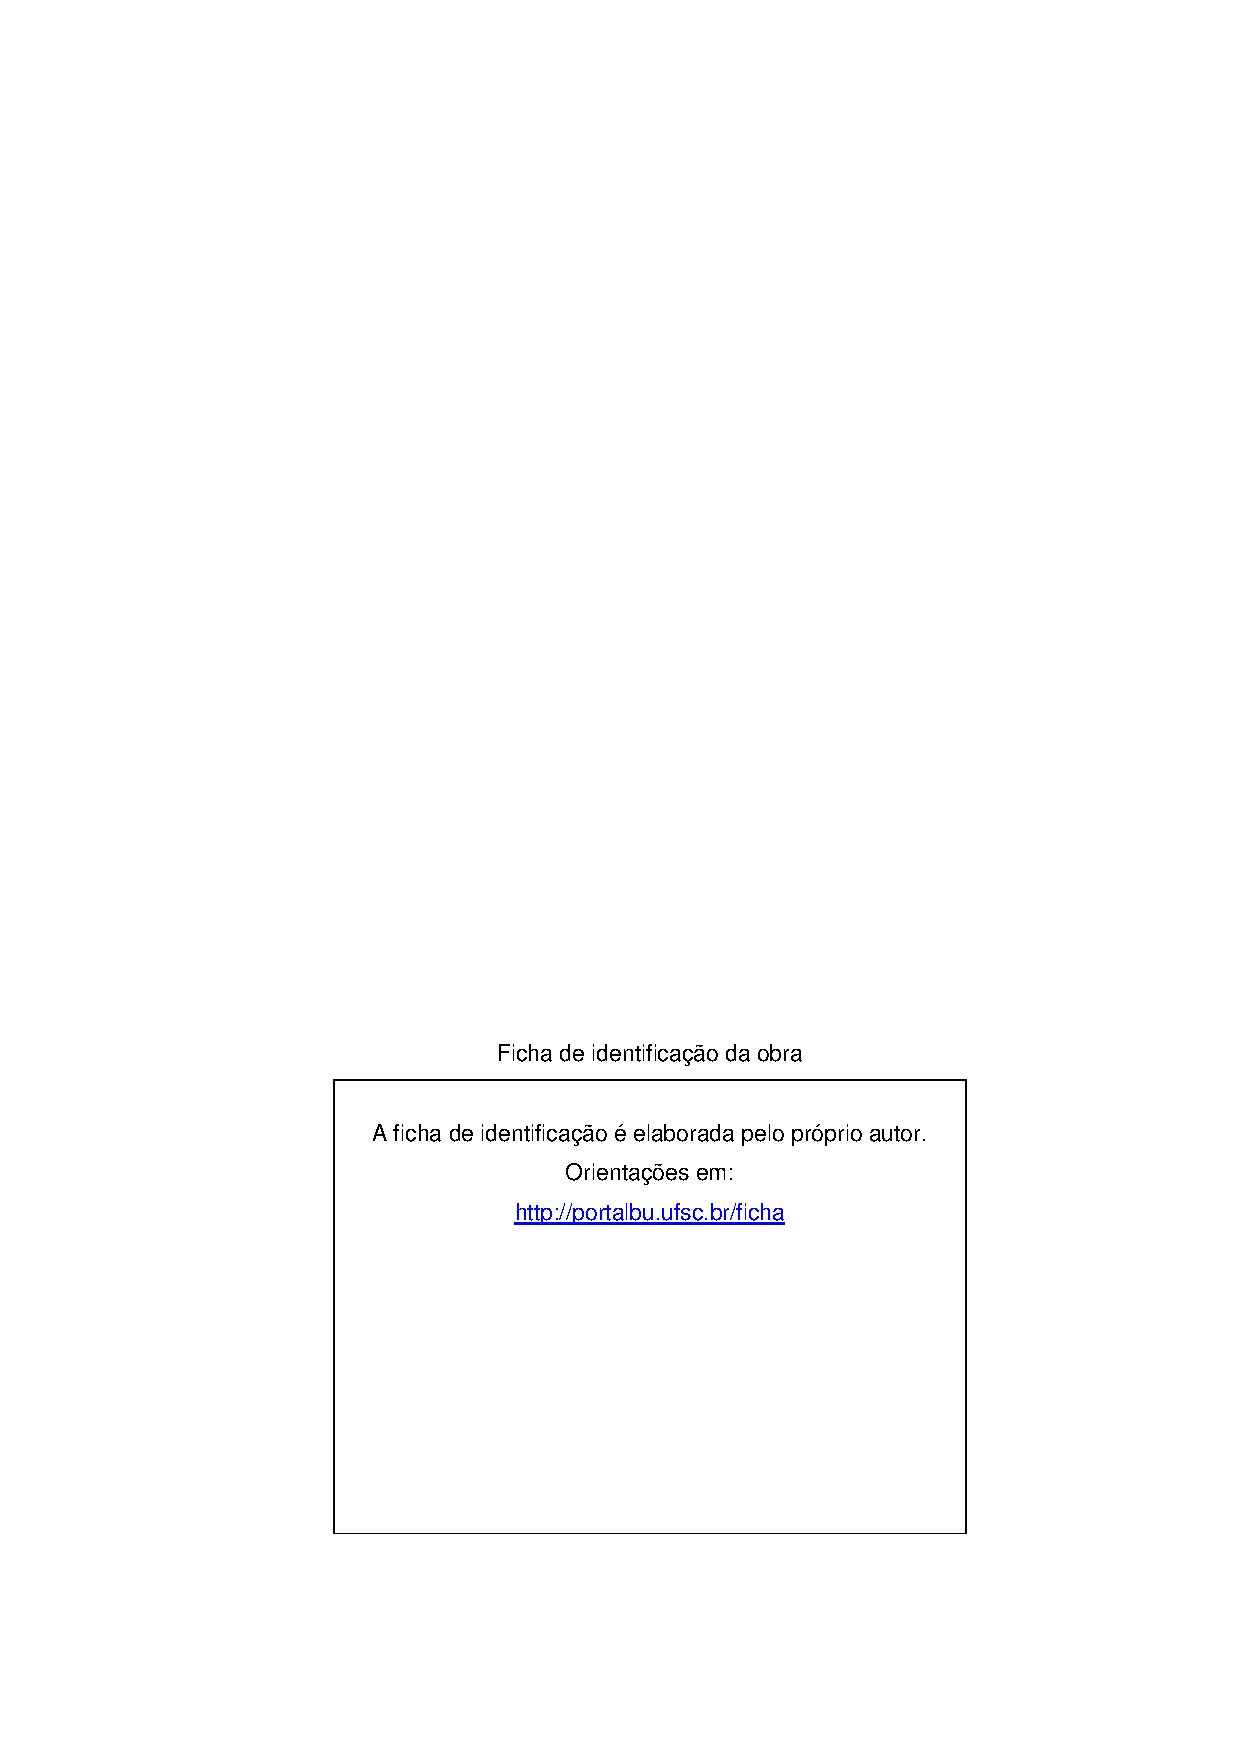
\includepdf{pictures/Ficha_Catalografica.pdf}
    %\ifforcedinclude\else\cleardoublepage\fi
\fi


% Inserir errata

% Inserir folha de aprovação. Isto é um exemplo de Folha de aprovação, elemento obrigatório da
% NBR 14724/2011 (seção 4.2.1.3). Você pode utilizar este modelo até a aprovação do trabalho.
% Após isso, substitua todo o conteúdo deste arquivo por uma imagem da página assinada pela
% banca com o comando abaixo:

\newpage 
\ % The empty page
\newpage

\ifforcedinclude\else\cleardoublepage\fi


\addtotextpreliminarycontent{\lang{Approval Sheet}{Folha de Aprovação}}

\begin{folhadeaprovacao}

    \begin{center}
        {\imprimirautor}

        \begin{center}
            \ABNTEXchapterfont\bfseries\MakeUppercase{Expert Bee: Um Sistema Especialista de Apoio ao Ensino Integrado ao Beecrowd}\ifnotempty{\imprimirsubtitulo}{: \imprimirsubtitulo}
        \end{center}

        \begin{minipage}{\textwidth}
            \lang
            {
                This \imprimirtipotrabalho~was considered appropriate to get the \imprimirformacao,
                \ifnotempty{\imprimirarea}{in the area of \imprimirarea,}
                and it was approved by the \imprimirprograma~of \imprimircentro~of \imprimirinstituicao.
            }
            {
                Este \imprimirtipotrabalho~foi julgado adequado para obtenção do Título de \imprimirformacao,
                \ifnotempty{\imprimirarea}{na área de concentração de \imprimirarea,}
                e foi aprovado em sua forma final pelo \imprimirprograma~
                do \imprimircentro~da \imprimirinstituicao.
            }
         \end{minipage}%
    \end{center}

    \begin{center}
        \imprimirlocal, \imprimirdata.
    \end{center}

    \assinatura{%
        \textbf{\imprimircoordenador} \\
        \imprimircoordenadorRotulo~\lang{of}{do} \imprimirprograma
    }

    \vspace*{1cm}

    % \newpage
    \begin{flushleft}
        \textbf{\lang{Examination Board}{Banca Examinadora}:}
    \end{flushleft}

    \vspace*{0.5cm}

    \begin{center}
        \assinatura{%
            \textbf{\imprimirorientador} \\ \imprimirorientadorRotulo\\
            \imprimirinstituicao~--~\imprimirinstituicaosigla
        }
        \vspace*{0.5cm}

        \ifnotempty{\imprimircoorientador}{%
            \assinatura{%
                \textbf{\imprimircoorientador} \\ \imprimircoorientadorRotulo \\
                \imprimirinstituicao~--~\imprimirinstituicaosigla
            }
        }

        \vspace*{0.5cm}

        \assinatura{%
            \textbf{Prof. Álvaro Junio Pereira Franco, \lang{PhD.}{Dr.}} \\
            Avaliador \\
            \imprimirinstituicao~--~\imprimirinstituicaosigla
        }
    
    \end{center}

    \vspace*{1cm}

    \begin{center}
        \assinatura{%
            \textbf{Profa. Luciana de Oliveira Rech, \lang{PhD.}{Dra.}} \\
            Avaliadora \\
            \imprimirinstituicao~--~\imprimirinstituicaosigla
        }
    \end{center}

\end{folhadeaprovacao}


% \includepdf{pictures/folhadeaprovacao_final.pdf}


% Dedicatória
%\ifforcedinclude\else\cleardoublepage\fi
%\ifforcedinclude\else

\addtotextpreliminarycontent{\lang{Dedicatory}{Dedicatória}}

\begin{dedicatoria}

    \vspace*{\fill}
    \centering
    \noindent
    \textit{\lang
    {
        This work is dedicated to adult children who, \\
        When small, dreamed of becoming scientists.
    }
    {
        Este trabalho é dedicado às crianças adultas que,\\
        quando pequenas, sonharam em se tornar cientistas.
    }}
    \vspace*{\fill}

\end{dedicatoria}


\fi

% Agradecimentos
%\ifforcedinclude\else\cleardoublepage\fi
%

\addtotextpreliminarycontent{\lang{Acknowledgement}{Agradecimentos}}

\begin{agradecimentos}

\lang
{
    Greetings.
}
{
    Agradeço a Deus pela força que me concedeu em toda essa caminhada, pois tudo posso naquele que me fortalece.

    Agradeço à minha família, e em especial aos meus pais, Valter e Ana, e à minha avó Denilce, por possibilitarem toda a minha trajetória acadêmica e pelo amparo incondicional.

    Agradeço ao meu namorado, Pedro, por estar ao meu lado desde o início dessa caminhada, me incentivando e apoiando.

    À Gabi e ao Dani, que sempre estiveram ao meu lado. Agradeço por todos os momentos compartilhados, e que venham muitos outros.

    Ao meu orientador, o professor Maicon, agradeço pela atenção, paciência e orientação, que foram essenciais para que o projeto fosse concluído.

    À UFSC e a todos os seus professores que sempre proporcionaram um ensino de alta qualidade.

    E a todos os meus amigos, que fizeram parte dessa trajetória e que estiveram ao meu lado nos momentos bons e nos difíceis. Vocês fizeram essa jornada ser mais leve e mais divertida.

}

\end{agradecimentos}


%Mesmo padrão da seção primária, porém sem indicativo numérico. Assim como: Dedicatória, Resumo, Abstract, Sumário, Listas, Referências, Apêndices e Anexos.
%
%
%Corpo do texto, fonte 10,5, justificado, recuo especial da primeira linha de 1 cm, espaçamento simples.
%


% Epígrafe
%\ifforcedinclude\else\cleardoublepage\fi
%

\addtotextpreliminarycontent{\lang{Epigraph}{Epigrafe}}

\begin{epigrafe}

\vspace*{\fill}\lang
{
    \begin{flushright}
        \textit{``Learn from yesterday, live for today, hope for tomorrow. The important thing is not to stop questioning.''} \\ Albert Einstein
    \end{flushright}
    \begin{flushright}
        \textit{``The true sign of intelligence is not knowledge but imagination.''} \\  Albert Einstein
    \end{flushright}
    \begin{flushright}
        \textit{``Peace cannot be kept by force; it can only be achieved by understanding.''} \\ Albert Einstein
    \end{flushright}
    \begin{flushright}
        \textit{``Whoever is careless with the truth in small matters cannot be trusted with important matters.''} \\ Albert Einstein
    \end{flushright}
    \begin{flushright}
        \textit{``Extraordinary claims require extraordinary evidence''} \\ Carl Sagan
    \end{flushright}
    \begin{flushright}
        \textit{``Catholic, which I was until I reached the age of reason.''} \\ George Carlin
    \end{flushright}
    \begin{flushright}
        \textit{``We made too many wrong mistakes.''} \\ Yogi Berra
    \end{flushright}
}
{
    \begin{flushright}
        \textit{``Assim como aquele pecado da juventude, este documento te perseguirá pelo resto da vida.''} \\ Enio Valmor Kassick
    \end{flushright}
    \begin{flushright}
        \textit{``Estupidez trará mais autoconfiança do que o conhecimento e a bravura juntas. \englishword{\showfont}''} \\ Adriano Ruseler
    \end{flushright}
}

\end{epigrafe}





% Ajusta o espaçamento dos parágrafos do resumo
\setlength{\absparsep}{18pt}

% RESUMOS
\ifforcedinclude\else\cleardoublepage\fi


\newcommand{\imprimirbrazilabstract}{%
    \cleardoublepage\phantomsection
    \addtotextpreliminarycontent{Resumo em Português}
    \begin{otherlanguage*}{brazil}
    \begin{resumo}[Resumo]

        A utilização da tecnologia na educação tem o potencial de fortalecer a relação de ensino e aprendizagem entre educadores e alunos, 
        permitindo o acesso a materiais, cronogramas e fóruns por meio de ambientes virtuais. O Moodle é um exemplo de plataforma virtual 
        que oferece suporte pedagógico a instituições de ensino, e é amplamente utilizado dentre as universidades. Ele, além de simular 
        uma sala de aula online, possui ferramentas de suporte a cursos da área de Tecnologia da Informação e da Computação, como o VPL. 
        O VPL é um módulo integrado ao Moodle e gerenciador de tarefas de programação, mas que apresenta algumas limitações relacionadas à interface e à usabilidade. 
        Em contrapartida, existem plataformas não vinculadas ao Moodle que possuem um juiz online para problemas de programação, como o Beecrowd. 
        O Beecrowd, ao possuir questões prontas de programação, cada uma com baterias de testes, que fornecem feedback em tempo real, 
        permite aos usuários desenvolver habilidades de programação e resolução de problemas. Além disso, essa plataforma desperta um interesse 
        crescente nos ambientes pedagógicos. Isso ocorre, em parte, devido à sua vasta coleção de questões e também por estar disponível em 
        português brasileiro. Isso torna a plataforma acessível a um público mais amplo, especialmente àqueles que estão dando os primeiros 
        passos na área e ainda não possuem proficiência em inglês. Dessa forma, o objetivo deste trabalho consiste em favorecer 
        o uso da plataforma Beecrowd entre docentes, aproveitando a integração LTI já existente entre o Moodle e o Beecrowd, desenvolvida 
        pela equipe da plataforma. Além disso, busca-se disponibilizar uma ferramenta baseada em sistema especialista para auxiliar professores 
        e alunos no esclarecimento de dúvidas recorrentes sobre questões do Beecrowd, facilitando a adaptação de ambos ao uso da plataforma.

        \imprimirpalavraschave{Palavras-chaves}{\begin{inparaitem}[]\palavraschaveportugues\end{inparaitem}}

    \end{resumo}
    \end{otherlanguage*}
}


\newcommand{\imprimirenglishabstract}{%
    % https://tex.stackexchange.com/questions/20987/changing-babel-package-inside-a-single-chapter
    % https://tex.stackexchange.com/questions/36526/multiple-language-document-babel-selectlanguage-vs-begin-endotherlanguage
    \cleardoublepage\phantomsection
    \addtotextpreliminarycontent{English's Abstract}
    \begin{otherlanguage*}{english}
    \begin{resumo}[Abstract]

        The use of technology in education has the potential to strengthen the teaching and learning relationship between educators and students, 
        allowing access to materials, timetables and forums through virtual environments. Moodle is an example of a virtual platform that offers 
        pedagogical support to educational institutions, and is widely used among universities. As well as simulating an online classroom, it has 
        tools to support Information Technology and Computing courses, such as VPL. VPL is a Moodle-integrated module and programming task manager,
        but it has some limitations related to interface and usability. On the other hand, there are platforms not linked to Moodle that have an online judge for
        programming problems, such as Beecrowd. Beecrowd, by having ready-made programming questions, each with test batteries, which provide 
        real-time feedback, allows users to develop programming and problem-solving skills. In addition, this platform is attracting growing 
        interest in educational environments. This is partly due to its vast collection of questions and also because it is available in Brazilian 
        Portuguese. This makes the platform accessible to a wider audience, especially those who are taking their first steps in the field and are 
        not yet proficient in reading English. Therefore, the aim of this study is to favor the use of the Beecrowd platform among educators, 
        leveraging the existing LTI integration between Moodle and Beecrowd, developed by the platform's team. Additionally, it aims to provide 
        a tool based on an expert system to assist both teachers and students in clarifying recurring doubts about Beecrowd problems, facilitating 
        their adaptation to the platform.

        \imprimirpalavraschave{Keywords}{\begin{inparaitem}[]\palavraschaveingles\end{inparaitem}}

    \end{resumo}
    \end{otherlanguage*}
}


% \newcommand{\imprimirfrenchabstract}{%
%     \addtotextpreliminarycontent{Français Résumé}
%     \begin{resumo}[Résumé]
%       \begin{otherlanguage*}{french}
%           Il s'agit d'un résumé en français.

%           \imprimirpalavraschave{Mots-clés}{latex. abntex. publication de textes.}
%       \end{otherlanguage*}
%     \end{resumo}
% }


% \newcommand{\imprimirspanishabstract}{%
%     \addtotextpreliminarycontent{Español Resumen}
%     \begin{resumo}[Resumen]
%       \begin{otherlanguage*}{spanish}
%           Este es el resumen en español.

%           \imprimirpalavraschave{Palabras clave}{latex. abntex. publicación de textos.}
%       \end{otherlanguage*}
%     \end{resumo}
% }


\makeatletter
\ifenglish
    \@ifundefined{imprimirbrazilabstract}{}{\imprimirbrazilabstract}

    % https://tex.stackexchange.com/questions/331108/times-new-roman-in-latex-just-some-text
    % https://tex.stackexchange.com/questions/11707/how-to-force-output-to-a-left-or-right-page
    % https://tex.stackexchange.com/questions/132966/do-not-display-chapter-title-in-memoir-class
    \cleardoublepage\phantomsection
    \pretextualchapter{Resumo Expandido}
    \addtotextpreliminarycontent{Resumo Expandido}

    \begin{otherlanguage*}{brazil}
        \setlength{\parskip}{0.2cm}
        \setlength{\parindent}{0.0cm}
        \fontfamily{ptm}\selectfont

        \section*{Introdução}
        O resumo expandido é previsto na Resolução Normativa nº 95/CUn/2017, Art. 55, § 2, de 4 de
        abril de 2017, e exigido para teses e dissertações escritas em idiomas estrangeiros (com
        exceção dos cursos pertinentes ao estudo de idiomas estrangeiros – Programa de Pós-Graduação
        em Estudos da Tradução e Programa de Pós-Graduação em Inglês: Estudos Linguísticos e
        Literários).

        O resumo expandido é considerado um elemento pré-textual e deverá ser incluído no trabalho
        após o resumo e antes do abstract. Deverá iniciar em página impar (no anverso de uma folha)
        continuando no verso da folha. O texto deverá seguir o formato A5, com margens espelhadas:
        superior 2,0 cm, inferior 1,5 cm, interna 2,5 cm e externa 1,5. Deve ser empregada a fonte
        Time New Roman.  Todo o texto deve ser digitado em tamanho 10,5. O espaçamento entre as
        linhas deverá ser simples. A expressão “resumo expandido” deve seguir a mesma tipografia das
        demais sessões primárias do trabalho.

        O texto do resumo expandido deve ser redigido em português e conter as seguintes seções (ver
        modelo): Introdução, Objetivos, Metodologia, Resultados e Discussão e Considerações Finais.
        Deve apresentar no mínimo duas (02) e, no máximo, cinco (05) páginas contendo a mesma
        formatação em A5 do resumo e do abstract, bem como palavras-chave. \englishword{\showfont}

        \section*{Objetivos}
        Lorem ipsum dolor sit amet, consectetur adipiscing elit. Phasellus vitae dolor lacus. Ut
        accumsan vitae felis nec porttitor. Integer interdum fringilla feugiat. Nullam pulvinar sit
        amet tellus eget maximus. Donec sit amet magna eget justo semper fermentum vel eget velit.
        In iaculis imperdiet mauris, ac ornare libero placerat non. Nulla libero lectus, ullamcorper
        ac ornare eget, pulvinar ac nulla. Curabitur vestibulum non nisl eget sagittis. Proin
        gravida lacus id eros bibendum interdum. Mauris ullamcorper elementum tortor sed consequat.
        Integer tempus, est a lobortis vehicula, nisi mi fringilla augue, non semper leo metus in
        quam. Etiam in leo maximus, pulvinar mi eget, vehicula risus. Donec sed dui semper, dictum
        eros at, suscipit felis.

        Nam sagittis vel orci at tempus. Nulla non pellentesque eros.
        Quisque cursus leo massa, eu ultricies nisl lacinia a. Nulla sit amet elementum ligula.
        Proin sodales venenatis dictum. Ut et est cursus, vulputate velit et, viverra odio. Interdum
        et malesuada fames ac ante ipsum primis in faucibus. Maecenas purus diam, tempor a semper
        et, finibus a ex. Cras sagittis felis urna, et consequat arcu lacinia ut. Praesent blandit
        venenatis ante nec porta. Duis rutrum, tellus vitae ullamcorper auctor, lectus ex laoreet
        est, ac tristique ipsum arcu vitae nibh. Nam efficitur felis ut mi consectetur, nec auctor
        odio ornare. In tempor vulputate urna, vitae cursus enim egestas eu. Proin diam augue,
        dignissim vitae ligula eget, lobortis ornare odio. Duis quis elit augue. Fusce quis rhoncus
        tortor. Donec hendrerit at massa a mattis. Sed ipsum neque, aliquam ut sem sed, ultrices
        varius ligula. Suspendisse blandit, dolor ac rhoncus lacinia, dolor purus cursus purus, et
        accumsan orci neque a leo.

        \section*{Metodologia}
        Quisque efficitur dolor in lectus dapibus elementum. Nam ultrices blandit consectetur.
        Nullam ultricies sit amet odio quis placerat. Aenean eget est elit. Maecenas et nulla dolor.
        Orci varius natoque penatibus et magnis dis parturient montes, nascetur ridiculus mus. In
        pulvinar velit sed mi sagittis ornare. Aenean rutrum suscipit egestas. Phasellus pharetra
        eget ex in volutpat. Quisque eu arcu nunc. Vivamus arcu ligula, pharetra at rhoncus sit
        amet, pulvinar sed eros. Sed porta ipsum ipsum, et fermentum magna volutpat sed. Vivamus
        pharetra facilisis orci, sit amet luctus nisl pretium id. Sed consequat, arcu et congue
        pulvinar, risus enim aliquet purus, eget venenatis libero leo sit amet metus. Maecenas vitae
        elit sapien. Fusce mollis libero et gravida placerat. Proin ut quam quis justo aliquam
        dictum. Donec volutpat convallis suscipit. Vivamus metus nisl, placerat ac enim vitae,
        tempus ultricies odio.

        Aliquam ac vehicula arcu, non bibendum nulla. Morbi libero sem,
        imperdiet vel quam et, posuere tempus nunc. Maecenas dictum magna sit amet ligula facilisis
        commodo. Aliquam tellus diam, ornare vel elementum in, dignissim id purus. Ut at tortor non
        sem molestie euismod non at turpis. Phasellus vitae bibendum tellus. Suspendisse odio enim,
        faucibus eget congue quis, semper sit amet tortor. Sed ac lectus est. Pellentesque nec
        mattis mi, et varius dolor. Aliquam quis massa ac tellus malesuada sollicitudin. Maecenas
        ultrices risus massa, nec auctor risus sagittis id. Praesent a sapien nulla. Donec
        tincidunt, metus quis hendrerit facilisis, enim augue convallis elit, sed consequat lacus
        odio vitae magna.

        \section*{Resultados e Discussão}
        Nullam sed cursus leo. Donec commodo volutpat hendrerit. Fusce et tempus lectus, feugiat
        consequat est. Class aptent taciti sociosqu ad litora torquent per conubia nostra, per
        inceptos himenaeos. Nam quis cursus mauris, non tempus orci. Phasellus lobortis et mauris at
        vulputate. Sed nec nisl elementum lorem commodo gravida non a enim. Phasellus neque erat,
        aliquet ac ligula ac, maximus vestibulum sem. Vestibulum vel tincidunt turpis. Donec lacinia
        rutrum dolor dapibus bibendum. Mauris pharetra nibh nec tincidunt iaculis. Vivamus pharetra
        bibendum nisl eget blandit. In lobortis diam non justo eleifend, id lobortis ante fringilla.
        Donec libero tortor, suscipit vestibulum vestibulum id, rutrum accumsan turpis. Phasellus
        sollicitudin luctus tincidunt. Suspendisse potenti. Nam semper metus et mi pharetra, in
        pretium ligula fermentum. Integer consectetur, orci non placerat feugiat, dui ex gravida
        augue, vel placerat ligula augue vel velit. Aliquam sollicitudin pellentesque congue. Donec
        vitae turpis in ante posuere posuere. Pellentesque eu justo leo. Donec quis elit vitae leo
        varius luctus quis eget justo.

        Vestibulum elementum ex neque, quis commodo tortor porttitor
        mattis. Mauris vel sagittis turpis. Aenean ligula turpis, eleifend at felis sed, cursus
        condimentum orci. Fusce accumsan est odio, eu venenatis massa sodales in. Curabitur a tempor
        nisl. Quisque consequat sed arcu a congue. In viverra, ex ut hendrerit condimentum, urna sem
        euismod eros, nec suscipit turpis dolor eget augue. Aenean posuere tellus et consectetur
        condimentum. Mauris et massa et nulla fringilla interdum. Duis quis posuere elit. Donec at
        ex non arcu faucibus rutrum et vel lectus. Vivamus pellentesque vestibulum rutrum. Sed
        pretium, purus sed efficitur feugiat, nisi justo eleifend nibh, id suscipit nunc massa nec
        lectus. In euismod enim eu sapien dictum sodales. Fusce sit amet vulputate orci. Nulla
        rutrum mauris at purus aliquet, ac sollicitudin leo laoreet. Etiam elementum posuere
        feugiat. Maecenas sed libero non augue fermentum ultricies eget at mi. Aenean auctor
        bibendum lacus, dignissim aliquet est tempus eget. Maecenas tempus, nulla id rhoncus
        suscipit, augue leo auctor mi, eget tincidunt magna mi quis dui. Maecenas ut elit in turpis
        tincidunt ultrices. Nulla id nulla aliquet, porttitor eros quis, egestas justo. Nunc nisi
        quam, egestas a accumsan fermentum, ultricies ac elit.

        Nulla porta auctor vestibulum. Sed
        consectetur lacus molestie iaculis ullamcorper. Proin porta posuere massa a lacinia. Nunc a
        lacinia orci, non vehicula ante. Vestibulum ipsum velit, congue et neque aliquam, imperdiet
        ornare augue. Donec et congue sapien. Pellentesque consequat consectetur neque ut varius. In
        aliquam ex quis ante venenatis dapibus. Vivamus et imperdiet urna. Vestibulum quis nibh
        magna. In a congue lectus, eu sodales nunc. Suspendisse id.

        \section*{Considerações Finais}
        Lorem ipsum dolor sit amet, consectetur adipiscing elit. Phasellus vitae dolor lacus. Ut
        accumsan vitae felis nec porttitor. Integer interdum fringilla feugiat. Nullam pulvinar sit
        amet tellus eget maximus. Donec sit amet magna eget justo semper fermentum vel eget velit.
        In iaculis imperdiet mauris, ac ornare libero placerat non. Nulla libero lectus, ullamcorper
        ac ornare eget, pulvinar ac nulla. Curabitur vestibulum non nisl eget sagittis. Proin
        gravida lacus id eros bibendum interdum. Mauris ullamcorper elementum tortor sed consequat.
        Integer tempus, est a lobortis vehicula, nisi mi fringilla augue, non semper leo metus in
        quam. Etiam in leo maximus, pulvinar mi eget, vehicula risus. Donec sed dui semper, dictum
        eros at, suscipit felis.

        Nam sagittis vel orci at tempus. Nulla non pellentesque eros.
        Quisque cursus leo massa, eu ultricies nisl lacinia a. Nulla sit amet elementum ligula.
        Proin sodales venenatis dictum. Ut et est cursus, vulputate velit et, viverra odio. Interdum
        et malesuada fames ac ante ipsum primis in faucibus. Maecenas purus diam, tempor a semper
        et, finibus a ex. Cras sagittis felis urna, et consequat arcu lacinia ut. Praesent blandit
        venenatis ante nec porta. Duis rutrum, tellus vitae ullamcorper auctor, lectus ex laoreet
        est, ac tristique ipsum arcu vitae nibh. Nam efficitur felis ut mi consectetur, nec auctor
        odio ornare. In tempor vulputate urna, vitae cursus enim egestas eu. Proin diam augue,
        dignissim vitae ligula eget, lobortis ornare odio. Duis quis elit augue. Fusce quis rhoncus
        tortor. Donec hendrerit at massa a mattis. Sed ipsum neque, aliquam ut sem sed, ultrices
        varius ligula. Suspendisse blandit, dolor ac rhoncus lacinia, dolor purus cursus purus, et
        accumsan orci neque a leo.


        \imprimirpalavraschave{Palavras-chaves}{\begin{inparaitem}[]\palavraschaveportugues\end{inparaitem}}

    \end{otherlanguage*}

    \@ifundefined{imprimirenglishabstract}{}{\imprimirenglishabstract}

\else
    \@ifundefined{imprimirbrazilabstract}{}{\imprimirbrazilabstract}
    \@ifundefined{imprimirenglishabstract}{}{\imprimirenglishabstract}
\fi

\@ifundefined{imprimirfrenchabstract}{}{\imprimirfrenchabstract}
\@ifundefined{imprimirspanishabstract}{}{\imprimirspanishabstract}
\makeatother



% Some tables of contents
\ifforcedinclude\else
{
    % https://tex.stackexchange.com/questions/179506/disable-colorlinks-locally-or-just-for-the-toc
    \hypersetup{hidelinks}

    % inserir lista de figuras
    \ifforcedinclude\else\cleardoublepage\fi
    % https://tex.stackexchange.com/questions/234398/list-of-figures-and-tables-when-there-are-no-figures-or-tables
    \whenlistisnotempty{\listfigurename}{%
        \addtotextpreliminarycontent{\listfigurename}
        % https://tex.stackexchange.com/questions/121879/remove-spacing-between-per-chapter-figures-in-lof
        {\renewcommand{\addvspace}[1]{}
        \listoffigures*}
    }{\pdfbookmark[0]{\listfigurename}{lof}}

    % inserir lista de quadros
    %\ifforcedinclude\else\cleardoublepage\fi
    % https://tex.stackexchange.com/questions/234398/list-of-figures-and-tables-when-there-are-no-figures-or-tables
    %\whenlistisnotempty{\listofquadrosname}{%
    %    \addtotextpreliminarycontent{\listofquadrosname}
        % https://tex.stackexchange.com/questions/121879/remove-spacing-between-per-chapter-figures-in-lof
    %    {\renewcommand{\addvspace}[1]{}
    %    \listofquadros*}
    %}{\pdfbookmark[0]{\listofquadrosname}{loq}}

    % inserir lista de tabelas
    \ifforcedinclude\else\cleardoublepage\fi
    % https://tex.stackexchange.com/questions/234398/list-of-figures-and-tables-when-there-are-no-figures-or-tables
    \whenlistisnotempty{\listtablename}{%
        \addtotextpreliminarycontent{\listtablename}
        % https://tex.stackexchange.com/questions/121879/remove-spacing-between-per-chapter-figures-in-lof
        {\renewcommand{\addvspace}[1]{}
        \listoftables*}
    }{\pdfbookmark[0]{\listtablename}{lot}}

    % inserir códigos fonte (List of Listings `lol`)
    % https://tex.stackexchange.com/questions/511519/latex-keeps-showing-minted-environment-as-figures-instead-of-listening/511579#511579
    %\ifforcedinclude\else\cleardoublepage\fi
    % https://tex.stackexchange.com/questions/234398/list-of-figures-and-tables-when-there-are-no-figures-or-tables
    %\whenlistisnotempty{\lstlistlistingname}{%
    %    \addtotextpreliminarycontent{\lstlistlistingname}
        % https://tex.stackexchange.com/questions/121879/remove-spacing-between-per-chapter-figures-in-lof
    %    {\renewcommand{\addvspace}[1]{}
    %    \lstlistoflistings*}
    %}{\pdfbookmark[0]{\lstlistlistingname}{lol}}
}
\fi


% inserir lista de abreviaturas e siglas
\ifforcedinclude\else\cleardoublepage\fi


\addtotextpreliminarycontent{\lang{List of Acronyms}{Lista de Siglas}}

\begin{siglas}
    \item[IDE] \lang{Integrated Development Environment}{\textit{Integrated Development Environment}}
    \item[URI] \lang{Integrated Regional University}{Universidade Regional Integrada}
    \item[VPL] \lang{Virtual Programming Lab}{\textit{Virtual Programming Lab}}
    \item[API] \lang{Application Programming Interface}{\textit{Application Programming Interface}}
    \item[VLE] \lang{Virtual Learning Environment}{\textit{Virtual Learning Environment}}
    \item[LMS] \lang{Learning Management System}{\textit{Learning Management System}}
    \item[SGBD] \lang{Database Management System}{Sistema Gerenciador de Banco de Dados}
    \item[AVA]  \lang{Ambiente Virtual de Aprendizagem}{Ambiente Virtual de Aprendizagem}
\end{siglas}



% Inserir lista de símbolos
%\ifforcedinclude\else\cleardoublepage\fi
%

\addtotextpreliminarycontent{\lang{List of Symbols}{Lista de Símbolos}}

% Devam aparecer na mesma ordem de ocorrência no texto.
\begin{simbolos}
    \item[$ \Gamma $] \lang{Greek letter Gama}{Letra grega Gama}
    \item[$ \Lambda $] \lang{Lambda}{Lambda}
    \item[$ \zeta $] \lang{Minimal Greek letter zeta}{Letra grega minúscula zeta}
    \item[$ \in $] \lang{Belongs}{Pertence}
\end{simbolos}


% How to remove the self-reference of the ToC from the ToC?
% https://tex.stackexchange.com/questions/10943/how-to-remove-the-self-reference-of-the-toc-from-the-toc
\ifforcedinclude\else\cleardoublepage\fi

\begin{KeepFromToc}
    % https://tex.stackexchange.com/questions/35/what-does-overfull-hbox-mean
    % https://tex.stackexchange.com/questions/59122/how-to-avoid-using-sloppy-document-wide-to-fix-overfull-hbox-problems
    % https://tex.stackexchange.com/questions/257007/adding-color-to-table-of-contents-and-section-headings
    {
        % https://tex.stackexchange.com/questions/179506/disable-colorlinks-locally-or-just-for-the-toc
        \hypersetup{hidelinks}

        % https://tex.stackexchange.com/questions/65711/underfull-vbox-badness-10000-with-memoir
        \raggedbottom

        % https://tex.stackexchange.com/questions/49887/overfull-hbox-warning-for-toc-entries-when-using-memoir-documentclass
        % \makeatletter
            % \renewcommand{\@pnumwidth}{2em}
            % \renewcommand{\@tocrmarg}{3em}
        % \makeatother

        % https://tex.stackexchange.com/questions/57544/memoir-mysterious-overfull-hbox-in-toc-when-mathptmx-is-used
        % \setlength{\cftchapternumwidth}{2.25em}

        % Add the table of contents to the brief table of contents
        % https://tex.stackexchange.com/questions/234398/list-of-figures-and-tables-when-there-are-no-figures-or-tables
        \whenlistisnotempty{\contentsname}{%
            \addtotextpreliminarycontent{\contentsname}
            \tableofcontents
        }{\pdfbookmark[0]{\contentsname}{toc}}
    }

\end{KeepFromToc}



    % ELEMENTOS TEXTUAIS
    \textual
    \setlength\beforechapskip{50pt}
    \setlength\midchapskip{20pt}
    \setlength\afterchapskip{20pt}

    % PARTE
    %\ifforcedinclude\else\part{\lang{Research}{Pesquisa}}\fi
    %\label{primeira_parte}

    % Introdução (exemplo de capítulo sem numeração, mas presente no Sumário)
    %% intro.tex
%%
%% Copyright 2017 Evandro Coan
%% Copyright 2012-2016 by abnTeX2 group at http://www.abntex.net.br/
%%
%% This work may be distributed and/or modified under the
%% conditions of the LaTeX Project Public License, either version 1.3
%% of this license or (at your option) any later version.
%% The latest version of this license is in
%%   http://www.latex-project.org/lppl.txt
%% and version 1.3 or later is part of all distributions of LaTeX
%% version 2005/12/01 or later.
%%
%% This work has the LPPL maintenance status `maintained'.
%% The Current Maintainer of this work is the Evandro Coan.
%%
%% The last Maintainer of this work was the abnTeX2 team, led
%% by Lauro César Araujo. Further information are available on
%% https://www.abntex.net.br/
%%
%% This work consists of a bunch of files. But originally there ware 3 files
%% which are renamed as follows:
%% Renamed the `abntex2-modelo-include-comandos` to `chapters/chapter_1.tex`
%% Renamed the `abntex2-modelo-trabalho-academico.tex` to `chapters/intro.tex`
%% Renamed the `abntex2-modelo-references.bib` to `aftertext/modelo-ufsc-references.bib`
%%
%% This file was originally the main template file, however this main file was
%% split into several new files, which are respectively drastically changed,
%% except this files which contains most of the main documentation message.
%%

% ------------------------------------------------------------------------
% ------------------------------------------------------------------------
% abnTeX2: Modelo de Trabalho Academico (tese de doutorado, dissertacao de
% mestrado e trabalhos monograficos em geral) em conformidade com
% ABNT NBR 14724:2011: Informacao e documentacao - Trabalhos academicos -
% Apresentacao
% ------------------------------------------------------------------------
% ------------------------------------------------------------------------

% The \phantomsection command is needed to create a link to a place in the document that is not a
% figure, equation, table, section, subsection, chapter, etc.
% https://tex.stackexchange.com/questions/44088/when-do-i-need-to-invoke-phantomsection
\phantomsection

% https://tex.stackexchange.com/questions/5076/is-it-possible-to-keep-my-translation-together-with-original-text
\chapter{\lang{Introduction}{Introdução}}
\phantomsection

% What does [t] and [ht] mean?
% https://tex.stackexchange.com/questions/8652/what-does-t-and-ht-mean
%
% How can I get rid of the LaTeX warning: Float too large for page?
% https://tex.stackexchange.com/questions/36252/how-can-i-get-rid-of-the-latex-warning-float-too-large-for-page
%
% "warning: Text page X contains only floats" How to suppress this warning?
% https://tex.stackexchange.com/questions/223149/warning-text-page-x-contains-only-floats-how-to-suppress-this-warning
%
% Make a table span multiple pages
% https://tex.stackexchange.com/questions/26462/make-a-table-span-multiple-pages
%
% How to make the longtable to work with centering & caption on memoir class?
% https://tex.stackexchange.com/questions/386541/how-to-make-the-longtable-to-work-with-centering-caption-on-memoir-class
%
% How to fix this Package array Error: Only one column-spec allowed?
% https://tex.stackexchange.com/questions/367069/how-to-fix-this-package-array-error-only-one-column-spec-allowed
%
% How to auto adjust my last table column width, and why is there Underfull \vbox badness on this table?
% https://tex.stackexchange.com/questions/387238/how-to-auto-adjust-my-last-table-column-width-and-why-is-there-underfull-vbox/387251
\setlength\extrarowheight{2pt}

% EXEMPLO DE TABELA
% \begin{tabularx}{\linewidth}{>{\RaggedRight}p{3cm}|>{\arraybackslash}X}

% \caption[Formatação do texto]{Formatação do texto \showfont}
% \label{tab:a_table_formatacao_de_texto} \\
% \hline
% \endfirsthead

% % How to set font size of footnotes correctly in memoir?
% % https://tex.stackexchange.com/questions/213927/how-to-set-font-size-of-footnotes-correctly-in-memoir
% \multicolumn{2}{p{\dimexpr\textwidth-2\tabcolsep\relax}}{\ufsccaptionsize\tablename~\thetable:
% Formatação do texto (continuação) \showfont} \\
% \hline
% \endhead

% % Set multicolumn width to default table width
% % https://tex.stackexchange.com/questions/99326/set-multicolumn-width-to-default-table-width
% \hline
% \multicolumn{2}{p{\dimexpr\textwidth-2\tabcolsep\relax}}{\footnotesize continua na próxima página\protect\englishword{\showfont}}
% \endfoot

% \hline
% \multicolumn{2}{p{\dimexpr\textwidth-2\tabcolsep\relax}}{\fonte{O autor -- \showfont} }
% \endlastfoot
%     Cor                          & Branco - \englishword{\showfont}                                 \\ \hline
%     Formato do papel             & A4                                                               \\ \hline
%     Gramatura                    & 75                                                               \\ \hline
%     Impressão                    & Frente e verso                                                   \\ \hline
%     Margens                      & Direita e superior 3, Inferior e esquerda: 2.                    \\ \hline
%     Cabeçalho                    & 0,7                                                              \\ \hline
%     Rodapé                       & 0,7                                                              \\ \hline
%     Paginação                    & Externa                                                          \\ \hline
%     Alinhamento vertical         & Superior                                                         \\ \hline
%     Alinhamento do texto         & Justificado                                                      \\ \hline
%     Fonte sugerida               & Times New Roman                                                  \\ \hline
%     Tamanho da fonte             & 12 para o texto incluindo os títulos das seções e subseções.
%                                    As citações com mais de três linhas as legendas das ilustrações
%                                    e tabelas, fonte 10.                                             \\ \hline
%     Espaçamento entre linhas     & Um e meio (1,5)                                                  \\ \hline
%     Espaçamento entre parágrafos & Anterior 0,0; Posterior 0,0                                      \\ \hline
%     Numeração da seção           & As seções  primárias devem  começar  sempre em páginas ímpares.
%                                    Deixar um espaço (simples) entre o título da seção e o texto e
%                                    entre o texto e o título da subseção.                            \\ \hline

% \end{tabularx}


% EXEMPLO DE FIGURA
% \begin{figure}
%     \caption{Exemplo de figura}
%     \label{fig:ex01}
%     \centering
%     \includegraphics[width=\linewidth]{pictures/ex01}
% \fonte{o autor -- \showfont}
% \end{figure}



A utilização da tecnologia no âmbito educacional aumenta o potencial de um vínculo proveitoso entre educadores e alunos, possibilitando a disponibilização de materiais, cronogramas, fóruns, entre outras atividades, por ambientes virtuais, e motivando, assim, os educandos  \cite[p.~18-19]{franciscojuniorambrosio}. Isto posto, há ambientes virtuais de aprendizado que servem de apoio às instituições de ensino no gerenciamento pedagógico dos cursos, como o software livre Moodle – (\textit{Modular Object-Oriented Dynamic Learning Environment}) – Ambiente de Aprendizagem Dinâmico Orientado a Objetos Modulares. O Moodle disponibiliza diversas ferramentas computacionais que proporcionam acesso a materiais didáticos, tarefas interativas e integração entre os membros do curso em que estão matriculados, reproduzindo, dessa forma, uma sala de aula \cite{limamoodle}. 

Por conseguinte, a fim de proporcionar uma maior assistência à cursos da área de tecnologia da informação, algumas iniciativas de integração de recursos de suporte à disciplinas de programação no ambiente Moodle foram elaboradas, como o VPL (\textit{Virtual Programming Lab})  \cite[p.~712]{franca2011}. 

O VPL é um módulo integrável ao Moodle que possibilita o desenvolvimento remoto de programas, permitindo realizar as seguintes atividades no navegador: editar o código-fonte dos programas, executá-los interativamente, realizar testes para revisá-los, definir restrições de edição e evitar colagem de texto externo \cite{rodriguezdelpino}. 

Contudo, \textcite[p.~129]{freitas} constata que, em sua pesquisa de avaliação do uso do VPL em disciplinas de programação no curso de graduação de Tecnologias de Informação e Comunicação da UFSC, apesar da ferramenta cumprir seu papel de auxílio virtual à prática de programação, ela possui diversos problemas de interface gráfica e de usabilidade. Destacou também falta de mensagens de ajuda apresentadas pela interface ao encontrar-se erros na submissão do código, a obrigatoriedade de casos de testes serem inseridos manualmente pelo criador da atividade, e a existência de botões não intuitivos para criação de atividades, como alguns dos defeitos encontrados, e sugeriu uma lista de melhorias necessárias nesse módulo.  Além disso, \textcite[p.~58]{freitas} cita que o VPL não permite o balanceamento de carga, já que há apenas um servidor responsável pela compilação e execução do código, podendo gerar um possível gargalo se muitos alunos submeterem trabalhos simultaneamente em um mesmo ambiente do Moodle. 

Em contrapartida, \textcite[p.~5]{cruz2022} destaca a plataforma Beecrowd como uma ferramenta que possibilita a resolução de problemas e desenvolvimento de algoritmos pelos alunos, ao mesmo tempo em que incentiva a participação em maratonas de programação e auxilia o educador na correção automatizada das respostas às questões. Do mesmo modo, \textcite[p.~239]{beztonin2014} mostram que a construção do Beecrowd (antigo URI Online Judge) foi inteiramente focada nas necessidades dos professores e, sobretudo, nas necessidades dos alunos. Nos aspectos didáticos e pedagógicos, é possível que o professor utilize o módulo acadêmico do portal a fim de fornecer aos alunos listas de exercícios, acompanhando o desempenho individual de cada um, podendo categorizar as listas por tema e estabelecer prazos para sua conclusão. Ainda, o portal possui recursos extremamente importantes para uma vida estudantil acadêmica, como “um nível de  problemas  para  iniciantes,  sistema  de  recompensa  por \textit{badges},  um  módulo  acadêmico completo  para  acompanhamento  de  listas  de  exercícios  pelos  alunos,  \textit{ranking}  dos  alunos  por Universidade, entre outros.” \cite[p.~239]{beztonin2014}. 

À vista disso, e ressaltando que o maior problema no ensino de algoritmos e programação para novos estudantes é atender com eficiência à grande diversidade de alunos e seus diferentes modos e ritmos de aprendizado \cite[p.~1]{beztonin2012}, “a possibilidade de utilização de ferramentas online com grande disponibilidade para aprendizagem ativa pode ser uma forma de possibilitar que cada aluno aprenda em seu próprio ritmo e velocidade” \cite[p.~5]{cruz2022}. Ademais, o uso de ferramentas online de auto aprendizado faz com que os educandos possam desenvolver suas habilidades de programação, desenvolvimento de código e solução de problemas com confiança e segurança, seguindo seu próprio ritmo de aprendizado \cite[p.~239-240]{beztonin2014}. 

\textcite[p.~248]{berssanettefrancisco}, salientou que o uso do Beecrowd contribui para o processo de aprendizagem de programação dos alunos ao proporcionar \textit{feedback} em tempo real aos estudantes e estimular a competitividade entre os alunos, por meio da gamificação presente na ferramenta, com \textit{badges} e \textit{ranking} dos estudantes. Também evidenciou o crescimento do anseio dos alunos por aprofundarem seus conhecimentos na resolução de problemas, e o envolvimento mais intenso dos mesmos na disciplina. Equitativamente, \textcite[p.~31]{ferreira2022} informa que a plataforma Beecrowd possui estudantes de mais de 240 países registrados, e frisou alguns dos seus recursos interessantes, como: a existência de uma base de problemas classificados em categorias e níveis de dificuldade, e a presença de um modelo de solução para cada problema, o qual é comparado com os dados de saída do programa do usuário, informando se o programa possui algum percentual de erro. 

De maneira geral, os alunos respondem de forma positiva ao \textit{feedback} imediato. No ambiente de laboratório, a rápida avaliação de cada pergunta motiva os alunos a buscar notas positivas, sendo raros os casos em que avançam sem corrigir eventuais erros. Eles apreciam a capacidade de acompanhar seu progresso durante todo o laboratório. Em exames, o feedback imediato elimina a incerteza sobre o desempenho, permitindo que os alunos saiam da sala de exame com clareza sobre suas notas \cite[p.~49]{lobbharlow}. 

Ainda, de acordo com \textcite[p.~24]{lima2023}, é notável que a plataforma Beecrowd seja uma das poucas no Brasil a disponibilizar questões em português brasileiro, o que a torna uma escolha significativa por parte dos professores para a utilização em sala de aula. Essa preferência amplia consideravelmente a acessibilidade do juiz online, beneficiando principalmente os iniciantes na área que ainda não possuem habilidades de leitura em inglês. 

Vale ressaltar que o autor também identificou duas outras plataformas, a Neps Academy e a CodeBench, que possuem questões em portugês brasileiro. Entretanto, essas alternativas não oferecem a mesma gama de recursos encontrados no Beecrowd. A Neps Academy, por exemplo, não permite o registro de turmas e a inscrição de alunos, funcionalidades que o Beecrowd oferece. Por outro lado, a CodeBench, embora seja amigável para professores e alunos, disponibiliza problemas privados. Nessa plataforma, apenas é possível visualizar as questões por meio de turmas com acesso restrito criadas pelos professores, o que impede que os alunos tentem resolver exercícios fora do ambiente de sala de aula \cite[p.~41]{lima2023}. 

Além disso, os autores \textcite[p.~41]{beztonin2012} testaram o uso dos juizes online BOCA e UVa Online Judge em sala de aula. Quanto ao BOCA, os professores explicaram que era necessário fazer uma limpeza no site a cada semestre, e novos problemas tinham de ser registrados. E, toda vez que isso tinha de ser feito, a classificação dos problemas e dos usuários eram perdidas. Já no uso do UVa Online Judge, apesar desse juiz conter uma enorme variedade de problemas em todos os assuntos de algoritmos, o período de manutenção do servidor geralmente coincidia com os horários das aulas, ficando off-line, e impossibilitando a dependência da ferramenta \cite[p.~1]{beztonin2012}. 

\textcite[p.~248]{beztonin2014} também registraram que, uma semana após o lançamento online da plataforma Beecrowd (conhecida como URI Online Judge na época), estudantes da área de Computação em todo o país já acessaram o portal, e, após um mês, os dados do Google Analytics revelaram a presença constante de usuários em todos os estados brasileiros e além-fronteiras. Após cerca de um ano e meio de operação, o Beecrowd mostrou-se sendo recebido, tanto nacional quanto internacionalmente, sendo regularmente utilizado por estudantes ao redor do globo, apresentando uma notável taxa de crescimento de usuários. 

Dessa maneira, ao considerar as limitações do módulo VPL, incluindo problemas de interface gráfica e usabilidade, e as desvantagens dos diversos juízes online mencionados anteriormente, destaca-se a popularidade do Beecrowd dentro e fora do Brasil, bem como seus diversos recursos avançados. Esses recursos foram desenvolvidos para atender às necessidades de alunos e professores, promovendo efetivamente o aprendizado. O crescente interesse da comunidade acadêmica em adotar o Beecrowd reflete uma demanda crescente por essa plataforma, que tem demonstrado sucesso em alcançar seus objetivos \cite[p.~31]{ferreira2022}. Portanto, deve-se estimular o uso do portal em ambientes acadêmicos, a fim de melhorar a qualidade do ensino de programação e resolução de problemas nas salas de aula.

\section{OBJETIVOS}

Neste contexto, o presente trabalho visa incentivar o uso da plataforma Beecrowd entre os docentes, aproveitando a integração LTI (Learning Tools Interoperability) já estabelecida entre o Moodle e o Beecrowd, desenvolvida pela equipe do Beecrowd. A LTI é um padrão que facilita a troca segura de dados entre o Sistema de Gestão de Aprendizado (LMS) e ferramentas de aprendizagem externas, centralizando o acesso a conteúdos internos e externos e facilitando logins entre diferentes plataformas \cite{verdaguer}. Assim, a LTI do Beecrowd permite que os usuários acessem o Beecrowd diretamente do Moodle, de maneira rápida e intuitiva por meio de um botão, tornando o uso da plataforma mais acessível e ágil.

Para complementar essa integração e oferecer um suporte abrangente, será disponibilizada uma aplicação web de apoio, com um sistema especialista que atende tanto professores quanto alunos. Para os professores, a ferramenta ajudará a esclarecer dúvidas frequentes dos alunos. Já para os alunos, ela permitirá que resolvam suas dúvidas de forma independente, sem depender da disponibilidade do professor.

Como as questões do Beecrowd podem ser reutilizadas a cada semestre em atividades de ensino e prática de programação, é comum que os alunos enfrentem dúvidas semelhantes ao resolverem esses problemas, o que gera um padrão previsível de questionamentos. Dada a diversidade de questões e os critérios rigorosos do sistema de correção do Beecrowd — que exige, por exemplo, formatação exata das respostas e a aprovação em múltiplos casos de teste —, essa ferramenta de apoio pretende facilitar a adaptação dos professores, fornecendo respostas a problemas comuns e orientações sobre as expectativas de correção do juíz online do Beecrowd, além de contribuir para uma melhor experiência de ensino e aprendizado na plataforma.

\subsection{\textbf{Objetivo Geral}}

Incentivar o uso da plataforma Beecrowd entre os docentes, para facilitar e aprimorar o ensino da prática de programação. Será aproveitada a integração LTI do Beecrowd com o ambiente Moodle já implementada, a qual facilita o acesso à plataforma e otimiza o aproveitamento de seu extenso banco de questões, oferecendo uma ampla variedade de exercícios de forma mais eficiente. Além disso, será disponibilizada uma ferramenta baseada em sistema especialista para auxiliar tanto professores quanto alunos no esclarecimento de dúvidas recorrentes sobre as questões do Beecrowd, facilitando a adaptação de ambos ao uso da plataforma.

\subsection{\textbf{Objetivos Específicos}}

\begin{enumerate}[label=(\alph*)]
    \item  Desenvolver um manual de instruções para auxiliar os professores no uso da LTI do Beecrowd, permitindo que compreendam e utilizem a ferramenta de forma eficaz, com ênfase nos recursos robustos do Beecrowd e seu vasto banco de questões;
    \item  Criar uma plataforma com um sistema especialista voltado ao esclarecimento de dúvidas frequentes dos alunos sobre as questões do Beecrowd. Este sistema atenderá as dúvidas recorrentes que surgem ao longo do semestre, já que muitas questões e suas respectivas dificuldades permanecem semelhantes;
    \item  Elaborar um manual de instruções para orientar os docentes no processo de adicionar respostas a novas dúvidas no sistema especialista.
\end{enumerate}

\section{MÉTODOS DE PESQUISA}

Na seção de fundamentação teórica, realiza-se uma análise abrangente sobre juízes online e suas aplicações no contexto acadêmico, com foco específico na plataforma Beecrowd e no BOCA Online Contest Administrator, investigando suas operações e funcionalidades. Nesta mesma seção, são relatadas e explicadas outras alternativas para o uso de ambientes auxiliares no ensino de programação, como o VPL e o CodeRunner, integrados ao AVA Moodle. Detalhes de funcionamento e execução de cada um são observados. Além disso, conduz-se uma análise aprofundada do ambiente AVA Moodle, explorando o conceito de LTI External Tools e suas relações com o Moodle, juntamente com os detalhes dos campos a serem preenchidos para a configuração de uma ferramenta externa LTI. Os conceitos LTI, Sistema Especialista e sua relação com a linguagem de programação Prolog e o projeto SWI-Prolog, e API também são expostos nessa seção, essenciais para o entendimento do desenvolvimento do sistema especialista. 

Na seção de trabalhos relacionados, realiza-se uma pesquisa bibliográfica sobre a integração de juízes online e outros ambientes de ensino de programação com o Moodle. O objetivo é avaliar a eficácia do juiz online Beecrowd na aprendizagem dos alunos, além de analisar como outros projetos semelhantes foram desenvolvidos, comparando suas abordagens com o presente trabalho. Adicionalmente, são discutidos dois estudos focados na criação de sistemas especialistas web, explorando suas características e destacando as principais diferenças em relação à proposta deste trabalho.

Na seção de desenvolvimento, são explorados os aspectos relacionados à LTI do Beecrowd, que facilita a integração entre o Moodle e a plataforma Beecrowd. Nessa etapa, são apresentados manuais detalhados para a configuração e utilização da LTI no Moodle. Além disso, a seção inclui diagramas, requisitos funcionais e não funcionais, bem como regras de negócio, que juntos definem a arquitetura geral do sistema especialista desenvolvido. Também são descritas as tecnologias selecionadas para o desenvolvimento, acompanhadas de uma explicação detalhada sobre a implementação da aplicação web do sistema especialista. Por fim, são exibidas imagens ilustrando o resultado final da aplicação.

Na seção de validação, será realizada uma análise da proposta, destacando as vantagens e desvantagens de utilizar a integração LTI entre o Moodle e o Beecrowd, bem como os benefícios e limitações de empregar um sistema especialista para resolver dúvidas relacionadas às questões do Beecrowd. Além disso, essa seção apresentará uma avaliação prática do uso da aplicação pelos alunos da disciplina \textit{Programação Orientada a Objetos I} da UFSC, no segundo semestre de 2024, verificando se as dúvidas dos estudantes foram efetivamente resolvidas pelo sistema especialista.

Por fim, na seção de conclusão, será apresentado um resumo das principais ações realizadas ao longo do trabalho, com ênfase na integração do Moodle com o Beecrowd por meio de LTI e no desenvolvimento da ferramenta com sistema especialista para apoiar os alunos. Além disso, serão discutidas as possibilidades de trabalhos futuros, com sugestões de aprimoramentos e novas direções para a ferramenta.

\section{ESTRUTURA DO TRABALHO}

A estrutura deste trabalho é organizada da seguinte maneira: a seção de Fundamentação Teórica apresenta os conceitos essenciais para compreender o desenvolvimento do projeto. Em Trabalhos Relacionados, são comparadas abordagens de integração de juízes online com o Moodle, além de artigos que tratam do desenvolvimento de sistemas especialistas web. O capítulo de Desenvolvimento apresenta a arquitetura da integração LTI, as tecnologias utilizadas e a implementação do sistema especialista. Na seção de Validação, são avaliadas as vantagens e limitações do sistema. A Conclusão discute um resumo das ações realizadas no trabalho e apresenta sugestões para trabalhos futuros.


    % Capitulo com exemplos de comandos inseridos de arquivo externo
    %% chapters/chapter_1.tex
%%
%% Copyright 2017 Evandro Coan
%% Copyright 2012-2014 by abnTeX2 group at http://abntex2.googlecode.com/
%%
%% This work may be distributed and/or modified under the
%% conditions of the LaTeX Project Public License, either version 1.3
%% of this license or (at your option) any later version.
%% The latest version of this license is in
%%   http://www.latex-project.org/lppl.txt
%% and version 1.3 or later is part of all distributions of LaTeX
%% version 2005/12/01 or later.
%%
%% This work has the LPPL maintenance status `maintained'.
%%
%% The Current Maintainer of this work is the Evandro Coan.
%%
%% The last Maintainer of this work was the abnTeX2 team, led
%% by Lauro César Araujo. Further information are available on
%% https://www.abntex.net.br/
%%
%% This work consists of a bunch of files. But originally there were 2 files
%% which are renamed as follows:
%% Deleted the `abntex2-modelo-img-marca.pdf`
%% Renamed the `abntex2-modelo-include-comandos.tex, v-1.9.2 laurocesar` to `chapters/chapter_1.tex`
%%
% ---
% Este capítulo, utilizado por diferentes exemplos do abnTeX2, ilustra o uso de
% comandos do abnTeX2 e de LaTeX.
% ---

% The \phantomsection command is needed to create a link to a place in the document that is not a
% figure, equation, table, section, subsection, chapter, etc.
% https://tex.stackexchange.com/questions/44088/when-do-i-need-to-invoke-phantomsection
\phantomsection

% https://tex.stackexchange.com/questions/5076/is-it-possible-to-keep-my-translation-together-with-original-text
\chapter{\lang{Theoretical Foundations}{Fundamentação Teórica}}

Neste capítulo, são apresentados os conceitos necessários para a compreensão da proposta. Serão mostrados tópicos como: juízes online, destacando o impacto dessa tecnologia na formação dos estudantes; Beecrowd, detalhando suas funcionalidades como plataforma de avaliação; BOCA \textit{Online Contest Administrator}, VPL (\textit{Virtual Programming Lab}) e \textit{CodeRunner},  ferramentas de apoio ao aprendizado de programação, mas apresentam limitações para o uso em sala de aula. Em seguida, será apresentado o Moodle, com ênfase em suas características gerais e na administração de cursos, usuários e \textit{sites}. A integração de ferramentas externas por meio de LTI também será abordada, destacando sua importância na interoperabilidade entre sistemas. Por fim, o capítulo abordará o conceito de web API, explicando seus fundamentos e funcionamento básico.

\section{Juízes Online}

Os autores \textcite{wasik} definem os juízes online como “sistemas projetados para a avaliação confiável do código-fonte do algoritmo enviado pelos usuários, que é compilado e testado em seguida em um ambiente homogêneo”. Da mesma forma, \textcite[p.~1]{santosribeiro} explicam a principal função dos juízes online: “avaliar códigos fonte que foram enviados em uma determinada linguagem de programação”. Essa avaliação automática é feita a partir de casos de teste, ou seja, cada caso de teste possui um conjunto de entradas e saídas, e verifica-se as respostas aos casos de teste da solução do usuário, com as respostas cadastradas para aquela questão no \textit{site} \cite[p.~12]{franciscojuniorambrosio}. 

Diversos juízes online podem ser encontrados na Internet, dentre eles estão o Beecrowd \cite{cruz2022} e o Codebench \cite[p.~806]{ribeirofernandescarvalho}, plataformas online com problemas de programação competitiva, e que aceitam soluções para esses desafios, avaliando-as quanto à sua eficácia e eficiência. Também há o BOCA \textit{Online Contest Administrator}, um sistema que visa apoiar as competições de programação na correção de soluções apresentadas pelos competidores \cite{camposferreira}. 

\textcite[p.~807-808]{ribeirofernandescarvalho} expôs que o Codebench é utilizado na UFAM (Universidade Federal do Amazonas) para dar suporte a professores e estudantes em disciplinas iniciais de programação. Assim, por meio desse sistema, professores e tutores das disciplinas podem disponibilizar exercícios de programação, listas e até mesmo provas para seus alunos, que, por sua vez, podem desenvolver soluções em uma IDE (\textit{Integrated Development Environment}) acoplada ao próprio sistema. Consequentemente, após a adoção do Codebench como ferramenta de apoio a uma metodologia de ensino híbrido de programação na UFAM, houve um aumento no índice de aprovações dos alunos da disciplina Introdução à Programação de Computadores \cite[p.~148-149]{galvaofernandesgadelha}.

Semelhantemente, \textcite[p.~18-19]{franciscojuniorambrosio} ressaltam os benefícios da utilização de um juiz online no ensino de matérias iniciais de programação: “[...] Aprendizagem no ritmo do aluno, auto-aprendizagem e redução da carga de trabalho do professor, são alguns dos benefícios apontados que contribuem não só em ambientes tradicionais de ensino, mas em ambientes de Educação a Distância (EAD) e em MOOC’s. A liberdade de definir listas de exercícios e a disponibilidade de instrumentos para acompanhar os alunos são questões importantes para o professor”.

Da mesma maneira, o desempenho dos estudantes do curso de Engenharia de Software da Universidade de Brasília foi influenciado diretamente pelo uso de problemas da maratona de programação e de juízes eletrônicos: observou-se que 50,3\% dos alunos apresentaram um aumento no desempenho em disciplinas de programação \cite[p.~218]{salescosta}.

Sob outra perspectiva, o desenvolvimento dos juízes online também é voltado ao uso em competições de programação \cite[p.~964-965]{santosribeiro}, já que são utilizados juízes eletrônicos, corretores automáticos de problemas, em maratonas de programação \cite[p.~34]{lima2023}. 

É interessante observar que o formato das questões em maratonas de programação é muito semelhante ao das questões em Juízes Online, e muitos dos exercícios disponíveis em Juízes Online originaram-se de competições de programação. Por conseguinte, a introdução dos estudantes a essas plataformas cria um ambiente mais familiar para as maratonas de programação, promovendo um engajamento positivo dos alunos com essa atividade e gerando impactos favoráveis em seu desempenho em disciplinas gerais de programação \cite[p.~33-34]{lima2023}.

Outrossim, \textcite[p.~2]{camposferreira} mostram as vantagens do incentivo à participação de alunos em competições de programação: “Competições de programação são uma excelente oportunidade para desenvolver nos alunos diversas habilidades que serão extremamente úteis no seu crescimento profissional. Nelas, os alunos aprendem de forma divertida conceitos importantes sobre estruturas de dados, algoritmos e desenvolvimento de software enquanto, ao mesmo tempo, aprendem a trabalhar em grupo e sob pressão” \cite[p.~2]{camposferreira}.

Portanto, além de seu papel essencial em competições de maratona de programação, os juízes online têm se destacado como ferramentas valiosas no ensino de programação básica. Como exposto acima, a integração dessas plataformas no ambiente educacional proporciona vantagens significativas, como a aprendizagem no ritmo do aluno e a facilidade dos professores em gerenciar uma turma. Portanto, essas ferramentas desempenham uma função fundamental na promoção do engajamento dos estudantes e no aprimoramento de seu desempenho em disciplinas gerais de programação, contribuindo significativamente para o campo educacional.


\section{Beecrowd}
\label{sec:beecrowd}

O Beecrowd, desde janeiro de 2013 até outubro de 2021 conhecido como URI Online Judge \cite[p.~5]{piekarski}, é um portal online criado com o objetivo principal de tornar a prática de programação mais dinâmica, interessante e estimulante para aqueles que acabaram de ingressar na arte de programar \cite[p.~1]{beztonin2012}.

A plataforma é um projeto desenvolvido na Universidade Regional Integrada - URI - Campus de Erechim, inicialmente com o intuito de criar um \textit{site} que tivesse um juiz automático, capaz de atender às necessidades dos professores e dos alunos, visando principalmente a interatividade, flexibilidade e novas fontes de informação e usabilidade \cite[p.~1]{beztonin2012}. O ambiente foi estruturado de forma a ser agradável, didaticamente organizado, e está disponível 24 horas por dia, oferecendo suporte tanto em inglês quanto em português \cite[p.~239]{beztonin2014}. A figura 1 mostra a página inicial do Beecrowd, após o usuário logar-se na plataforma.

\begin{figure}[h!]
	   \centering
            \caption{Portal Beecrowd - Home}
            \label{fig:BeecrowdHome}
	   	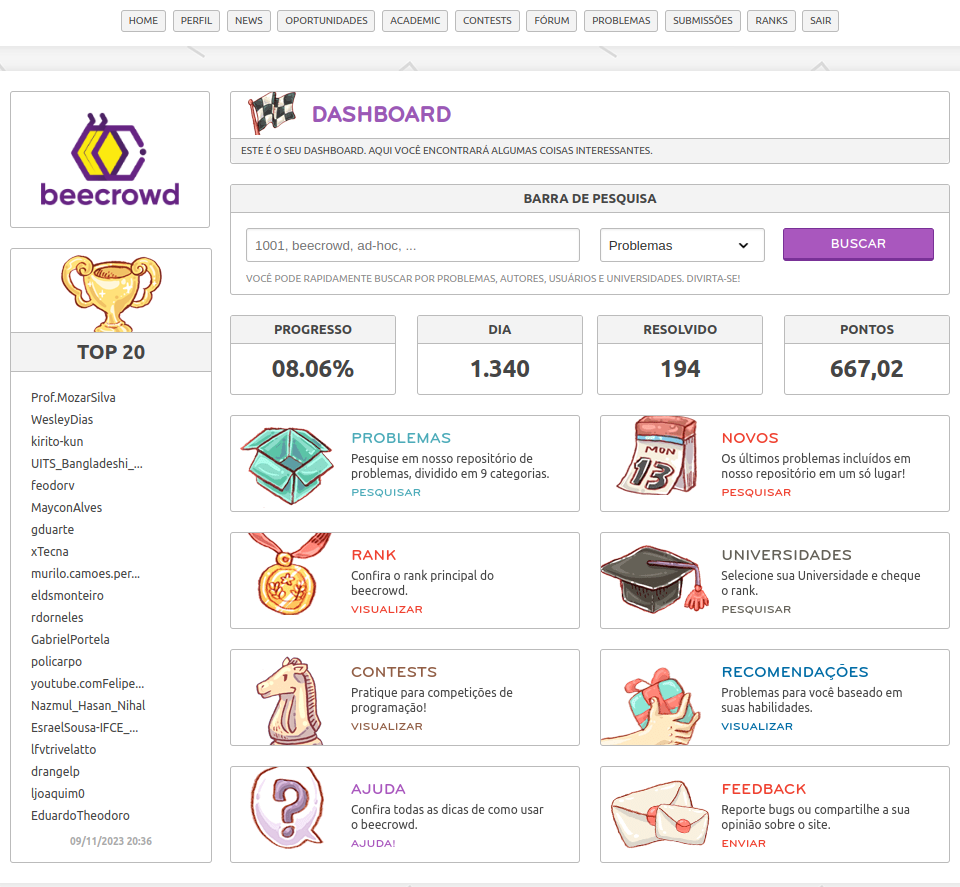
\includegraphics[scale=0.3]{pictures/beecrowd_home.png}
        \fonte{\cite{beecrowd}}
\end{figure}

Além disso, o Beecrowd contém problemas no estilo do ICPC - \textit{International Collegiate Programming Contest} da ACM, e disponibiliza um juiz online que avalia em tempo real as submissões dos algoritmos dos usuários \cite[p.~350]{berssanettefrancisco}. Os problemas são categorizados por assunto e por nível de dificuldade, e há flexibilidade na escolha da linguagem de programação com a qual se deseja resolver os exercícios \cite[p.~1]{beztonin2012}.

A figura 2 mostra as diferentes categorizações dos exercícios, que são: Iniciante: problemas básicos para quem está iniciando na programação; Ad-Hoc\footnote{\url{https://www.geeksforgeeks.org/what-are-ad-hoc-problems-in-competitive-programming/}}: problemas de simulação, datas e Ad-Hoc no geral; Strings: palíndromos, frequência, ad-hoc, LCS, manipulação de strings; Estruturas e Bibliotecas: filas, pilhas, ordenação, mapas; Matemática: sistemas numéricos, números primos, bigInteger; Paradigmas: programação dinâmica, busca binária, algoritmos gulosos, backtracking; Grafos: flood fill, MST, SSSP, DAG, fluxo máximo, árvores; Geometria Computacional: pontos e linhas, polígonos; e SQL: linguagens de consulta - seleção, inserção, atualização, criação.

\begin{figure}[h!]
	   \centering
            \caption{Portal Beecrowd - Categorias}
            \label{fig:ModeloConceitual}
	   	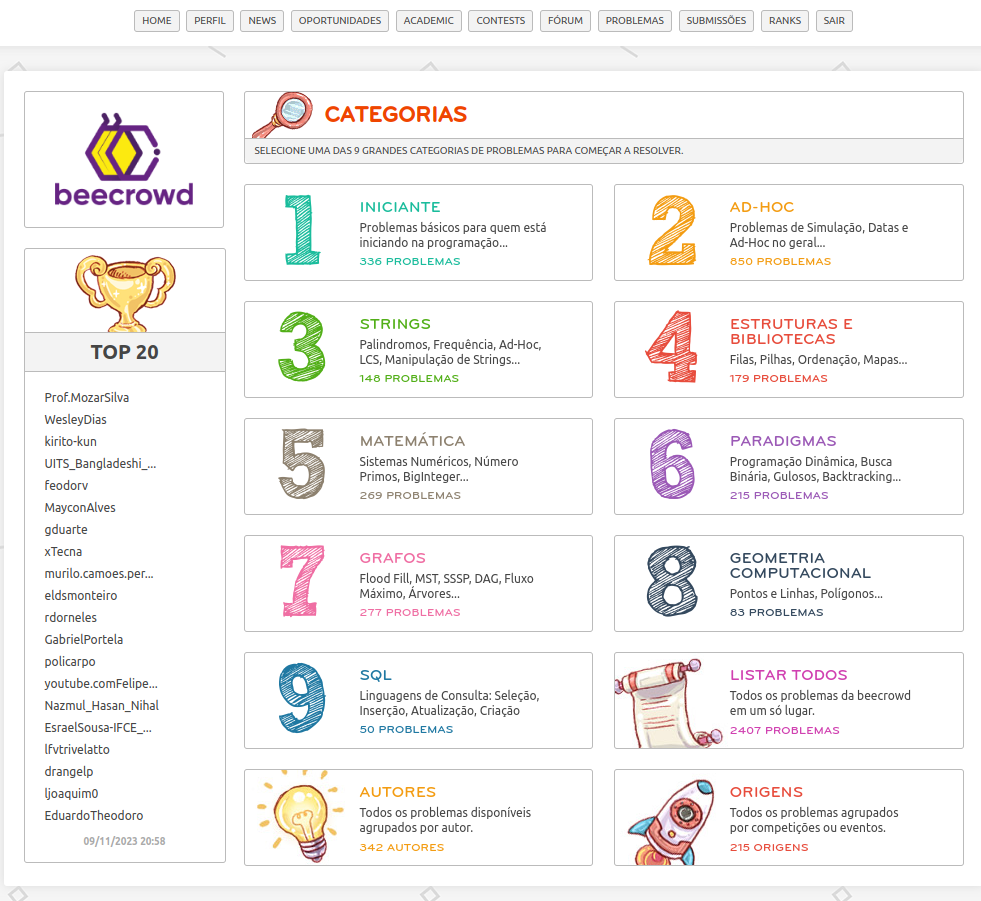
\includegraphics[scale=0.3]{pictures/beecrowd_problemas.png}
        \fonte{\cite{beecrowd}}
\end{figure}

Já na figura 3 estão listados diversos exercícios dentro da categoria Paradigmas, e, para cada problema, há um nível classificado (destacado na imagem com um retângulo azul). O nível representa a dificuldade da questão, e pode variar de 1 até 10, sendo 1 o nível mais fácil, e 10 o nível mais difícil \cite{beecrowd}. Dessa maneira, impede-se que estudantes iniciantes enfrentem frustrações ao tentar resolver problemas que demandam conhecimento mais avançado, prática e técnicas \cite[p.~239]{beztonin2014}.

\begin{figure}[h!]
	   \centering
            \caption{Portal Beecrowd - Exercícios dentro da categoria Paradigmas}
            \label{fig:ModeloConceitual}
	   	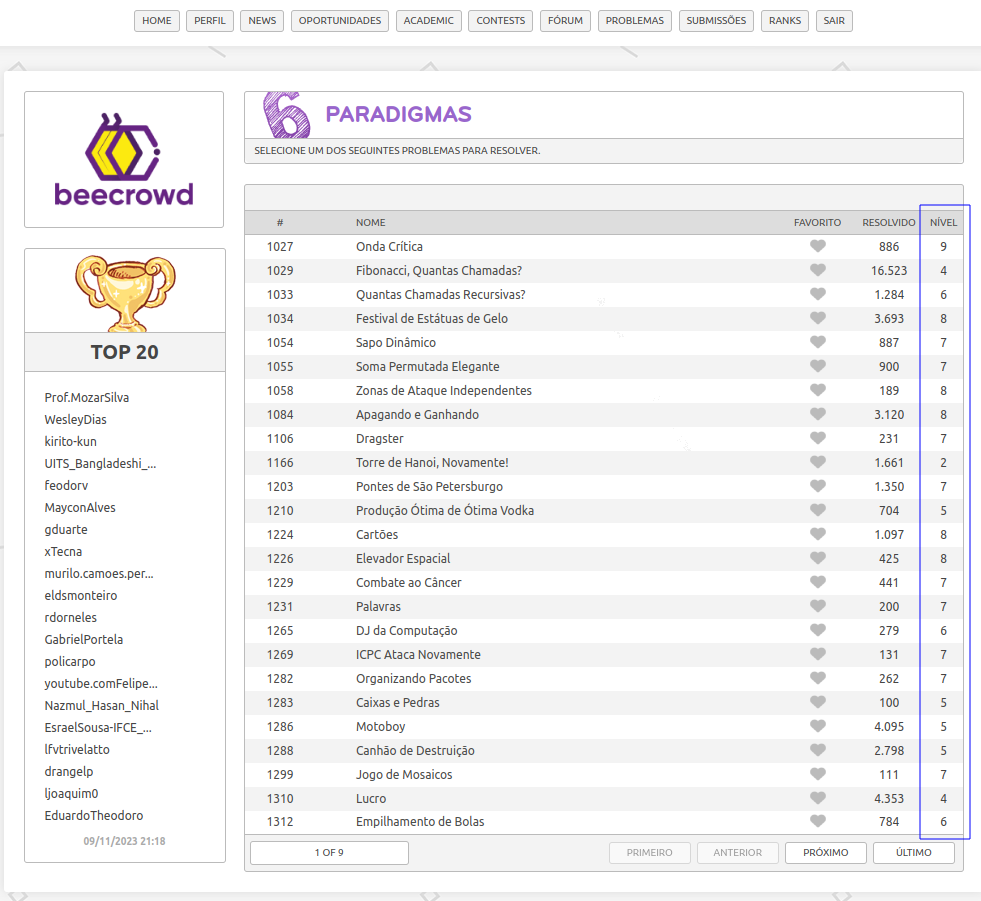
\includegraphics[scale=0.3]{pictures/beecrowd_paradigmas.png}
        \fonte{adaptado de \cite{beecrowd}}
\end{figure}

Ademais, o portal Beecrowd não apenas fornece uma plataforma desafiadora para competições de programação, mas também se destaca como um recurso educacional abrangente. Entre os seus diferenciais, evidenciam-se materiais de estudo, tutoriais sobre algoritmos e programação, e um fórum que facilita a colaboração entre os usuários. Além desses aspectos, o portal foi projetado com características específicas que o tornam uma ferramenta eficaz de apoio às aulas de Algoritmos e Estruturas de Dados. Por meio de problemas que abordam conceitos fundamentais dessas disciplinas, o Beecrowd oferece uma abordagem prática que contribui para uma compreensão mais sólida por parte dos estudantes \cite[p.~2]{beztonin2012}. 

A figura 4 mostra o fórum do exercício 1063 do Beecrowd, que pode ser acessado facilmente em Fórum -> Estruturas e Bibliotecas -> 1063, ou pelo próprio exercício 1063, no seu botão “Fórum”. Nesse fórum, diversas perguntas foram criadas para os alunos conversarem entre si sobre erros e problemas que tiveram.

\begin{figure}[h!]
	   \centering
            \caption{Portal Beecrowd - Fórum do Problema 1063}
            \label{fig:ModeloConceitual}
	   	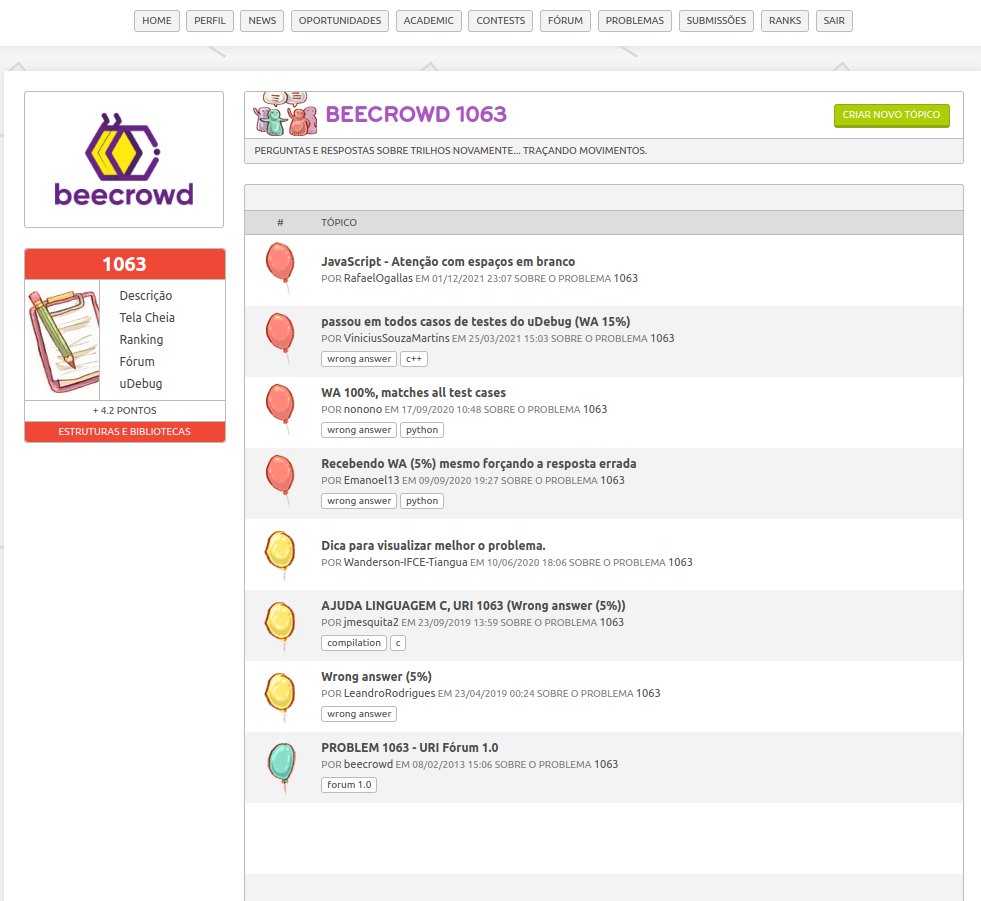
\includegraphics[scale=0.3]{pictures/beecrowd_1063.png}
        \fonte{\cite{beecrowd}}
\end{figure}

Além de ser um recurso fundamental para o aprimoramento das habilidades de programação dos alunos, o Beecrowd disponibiliza recursos diferenciados que se mostram valiosos para professores na área de Tecnologia da Informação. Essas características não apenas enriquecem o ambiente de aprendizado, mas também facilitam o processo de ensino e avaliação em cursos específicos dessa área. Os professores podem, por exemplo, criar disciplinas com alunos e listas de exercícios, separadas por assunto e delimitadas por prazos, caso desejado, e acompanhar a evolução dos alunos \cite[p.~239]{beztonin2014}.

Na figura 5 está a página Academic, do portal Beecrowd, onde alocam-se as disciplinas do usuário. Dentro de cada disciplina se encontram as listas de exercícios disponibilizadas aos alunos pelos professores, bem como algumas orientações aos usuários.

\begin{figure}[h!]
	   \centering
            \caption{Portal Beecrowd - Academic}
            \label{fig:ModeloConceitual}
	   	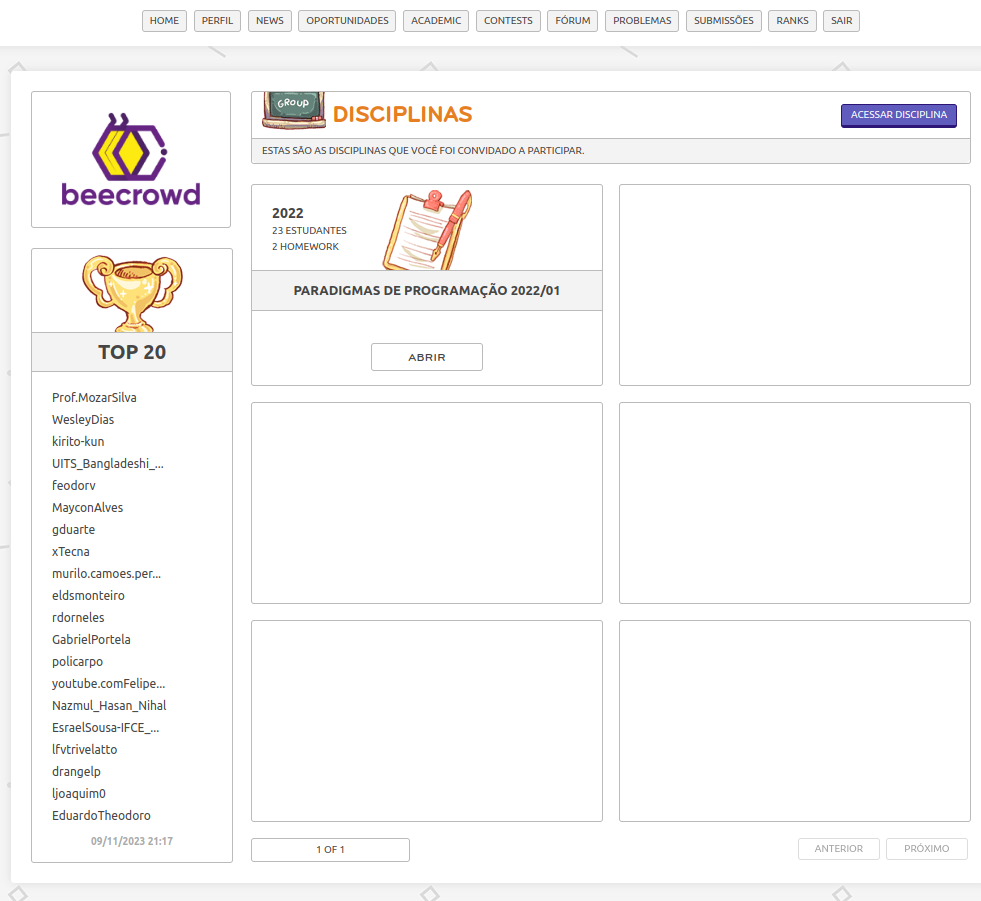
\includegraphics[scale=0.3]{pictures/beecrowd_academic.png}
        \fonte{\cite{beecrowd}}
\end{figure}

A construção do Beecrowd foi completamente centrada nas necessidades dos professores e, principalmente, nas necessidades dos alunos \cite[p.~239]{beztonin2014}. Ele integra recursos dos melhores portais de programação do mundo e, adicionalmente, oferece funcionalidades exclusivas, como um nível de problemas destinado a iniciantes, um sistema de recompensas por meio de \textit{badges}, e um módulo acadêmico completo para o acompanhamento das listas de exercícios, incluindo o \textit{ranking} de estudantes por universidade, entre outras inovações \cite[p.~239]{beztonin2014}.

A Figura 5 exemplifica um exercício do Beecrowd, o 1001: Extremamente Básico. Cada exercício é acompanhado por sua descrição, requisitos de entrada para o programa e a saída esperada do algoritmo a ser desenvolvido. Na seção à direita, o usuário pode selecionar a linguagem de programação desejada e utilizar a IDE integrada para desenvolver seu algoritmo. Ao concluir, o usuário deve clicar no botão "Enviar" para que a plataforma avalie sua solução. Após o envio, o aluno é redirecionado para uma tela onde o resultado é exibido na seção "Resposta" (Figura 6).

\begin{figure}[h!]
	   \centering
            \caption{Portal Beecrowd - Exercício 1001}
            \label{fig:ModeloConceitual}
	   	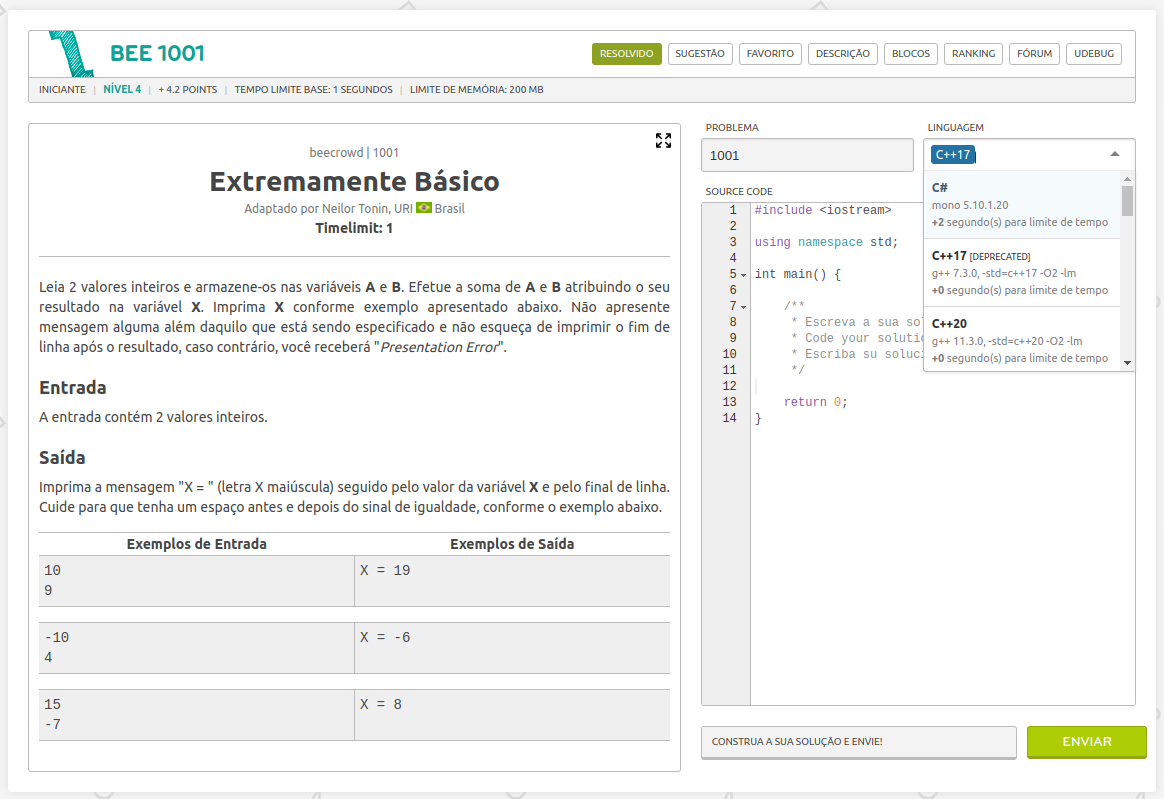
\includegraphics[scale=0.3]{pictures/beecrowd_1001.png}
        \fonte{\cite{beecrowd}}
\end{figure}

\begin{figure}[h!]
	   \centering
            \caption{Portal Beecrowd - Exercício Submetido}
            \label{fig:ModeloConceitual}
	   	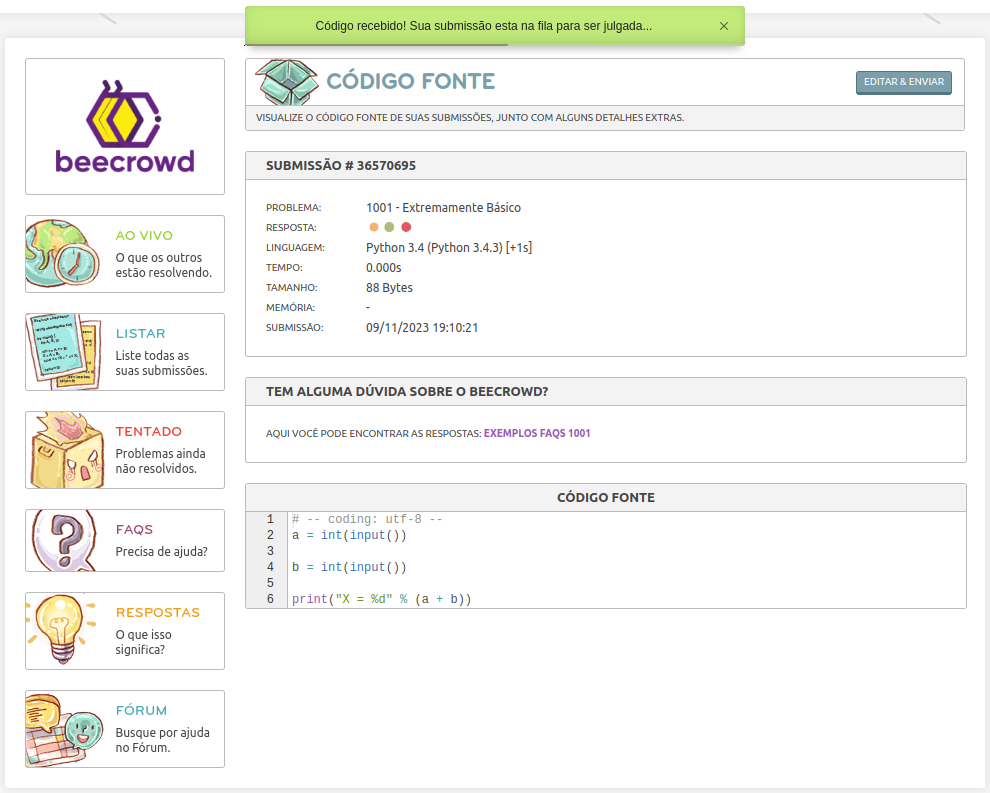
\includegraphics[scale=0.3]{pictures/beecrowd_submetido.png}
        \fonte{\cite{beecrowd}}
\end{figure}

As respostas possíveis do Juíz Online do Beecrowd são: \textit{Accepted, Compilation Error, Runtime Error, Time Limited Exceeded, Presentation Error, Wrong Answer, Closed}. O significado de cada resposta pode ser encontrado na plataforma, oferecendo ao usuário uma indicação do que pode estar incorreto em seu algoritmo \cite{beecrowd}.

O Beecrowd também possui o ambiente Academic, e é esse ambiente que fornece ao professor diversos recursos \cite{beecrowdacademic}, como:

\begin{itemize}
    \item Criar disciplinas, podendo convidar alunos para participar dela;
    \item Criar listas de exercícios e acompanhar facilmente o progresso de seus estudantes (Veja figura 8), podendo ter uma melhor visão sobre como eles estão aplicando os tópicos apresentados em aula e onde eles estão encontrando dificuldades;
    \item Selecionar exercícios de programação do banco de dados do Beecrowd para essas listas, o qual possui mais de 2.000 problemas distintos;
    \item Visualizar todas soluções enviadas pelos alunos para suas listas de exercícios através de uma organizada linha do tempo;
    \item Definir data de início, prazo e duração das listas, considerando somente as submissões recebidas durante o tempo determinado;
    \item Visualizar \textit{feedback} sobre soluções copiadas entre estudantes e de repositórios online.
\end{itemize}

\begin{figure}[h!]
	   \centering
            \caption{Portal Beecrowd Academic - Progresso dos Alunos}
            \label{fig:ModeloConceitual}
	   	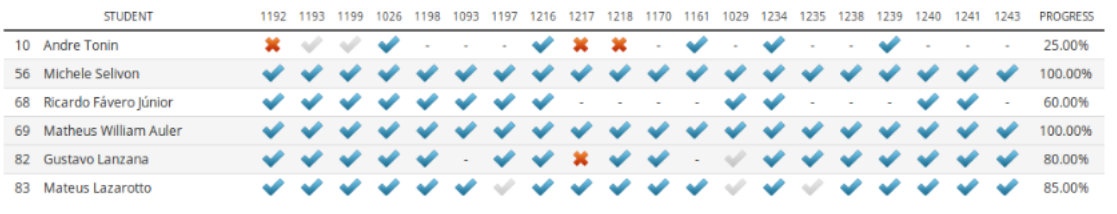
\includegraphics[scale=0.3]{pictures/beecrowd_academic_progresso.png}
        \fonte{\cite[p.~244]{beztonin2012}}
\end{figure}

Por fim, o Beecrowd oferece suporte a várias linguagens de programação e versões, dentre as quais o usuário pode escolher para desenvolver suas soluções. Todas essas linguagens estão listadas abaixo, na figura 9.

\begin{figure}[h!]
	   \centering
            \caption{Portal Beecrowd Academic – Linguagens e Versões}
            \label{fig:ModeloConceitual}
	   	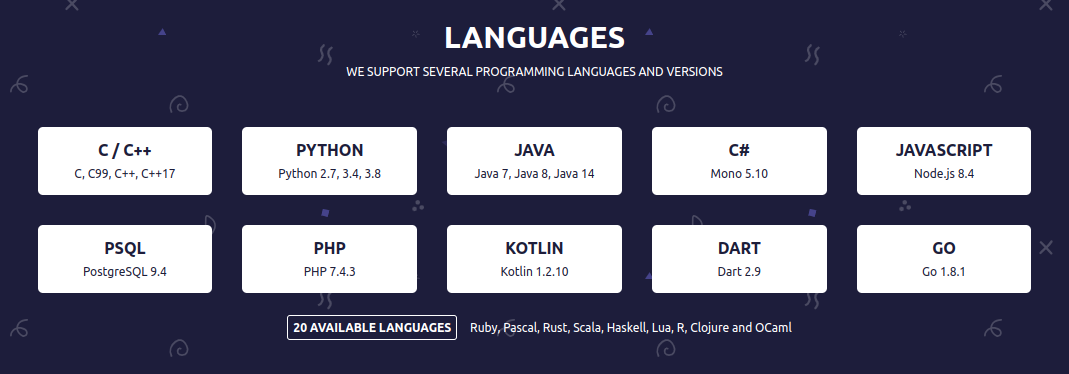
\includegraphics[scale=0.3]{pictures/beecrowd_academic_linguagens.png}
        \fonte{\cite{beecrowd}}
\end{figure}

\section{Boca Online Contest Administrator}

O BOCA \textit{Online Contest Administrator} é um ambiente utilizado para gerenciar competições que envolvem programação de computadores \cite[p.~22]{galasso}, e foi desenvolvido para ser usado na Maratona de Programação da Sociedade Brasileira de Computação \cite[p.~2]{camposferreira}.

Por ser um juiz online \cite[p.~1]{beztonin2012}, realiza a avaliação automática dos algoritmos submetidos, classificando-os como corretos ou incorretos \cite[p.~22]{galasso}. Ou seja, na competição, a correção dos programas enviados pelos times ocorre de forma online, e o resultado deve ser transmitido ao time o mais rápido possível. Após os competidores concluírem uma questão, enviam-na para o BOCA, que julga a solução fornecida e indica se está correta ou incorreta. Se estiver incorreta, o aluno tem a oportunidade de corrigi-la e submetê-la novamente, ainda durante o tempo da prova, mas sem ter conhecimento específico sobre o erro na questão \cite[p.~4]{camposferreira}. 

A utilização de interfaces web possibilita que o sistema BOCA seja aplicado na organização de competições distribuídas, permitindo que equipes estejam localizadas em qualquer lugar com acesso à internet. Essa abordagem é adequada para simulações e outras modalidades de competições \cite[p.~20]{camposferreira}.
 
Além disso, o BOCA proporciona a flexibilidade de ser utilizado em competições com várias sedes (ou \textit{sites}), todos operando simultaneamente, com a correção centralizada de submissões e dúvidas. Isso viabiliza competições em larga escala, alcançando regiões distantes de um país, como o Brasil, como evidenciado na Maratona de Programação. A centralização no processamento de submissões e dúvidas é essencial para assegurar igualdade de condições a todos os participantes, independentemente de sua localização, uma vez que tudo é processado pelo mesmo grupo de juízes \cite[p.~10-11]{camposferreira}.

Considerando que o BOCA foi desenvolvido apenas com o objetivo de auxiliar na avaliação de submissões de código em maratonas de programação, um benefício adicional do sistema é sua aplicabilidade no contexto de aprendizado, oferecendo suporte a disciplinas que envolvem a submissão e correção de trabalhos de programação \cite[p.~2]{camposferreira}. Por isso, ele foi utilizado por alunos de Ciência da Computação na URI por algum tempo, em sala de aula, para resolver problemas relacionados aos conteúdos abordados. Contudo, a cada semestre, era necessário realizar uma limpeza no \textit{site} e registrar novos problemas, incluindo todos os seus arquivos de entrada e saída, enunciado, e tempos limites, dependendo da matéria ensinada \cite[p.~1]{beztonin2012}. Os autores \textcite[p.~1]{beztonin2012}. destacaram que lidar com essa quantidade de problemas não é viável, pois o sistema não foi criado para esse propósito. Cada vez que o sistema era limpo, tanto a classificação dos problemas quanto a classificação dos usuários eram perdidas.

Assim, apesar de o BOCA não precisar de cadastro em nenhum portal, e ainda ter acesso a todo código fonte dos exercícios, ele não é a opção ideal para ser o sistema de juiz online utilizado em sala de aula. Ainda assim, o sistema revela-se uma escolha excelente para competições de programação. O crescimento extraordinário dessas competições tem despertado um interesse crescente entre os alunos de cursos de computação no Brasil. Esse interesse é extremamente positivo, pois motiva os alunos a estudarem conceitos fundamentais da computação, tais como estruturas de dados, análise de algoritmos, técnicas e linguagens de programação \cite[p.~11]{camposferreira}.

\section{VPL}

O Virtual Programming Lab (VPL) é um módulo de atividades para o Moodle que gerencia tarefas de programação \cite{vpl}. Suas características distintas incluem a capacidade de editar o código-fonte diretamente no navegador, permitindo aos alunos executar programas de forma interativa sem sair do ambiente Moodle. Tanto alunos quanto professores podem realizar testes para revisar os programas, enquanto a funcionalidade de pesquisa de similaridade entre arquivos auxilia na detecção de plágio. Além disso, o VPL oferece a possibilidade de definir restrições de edição e prevenir a colagem de texto externo, contribuindo para um ambiente acadêmico mais controlado e transparente \cite{vpl}.

Segundo \textcite[p.~1]{rodriguezdelpinoandroyo}, o VPL é um ambiente de desenvolvimento simples para os alunos, oferecendo recursos de avaliação automática. Para os instrutores, funciona como um sistema de gerenciamento do trabalho dos alunos, facilitando a preparação de tarefas, gerenciando envios, verificando plágio e conduzindo avaliações eficientes e flexíveis com base em testes de programas. Além disso, é independente da linguagem de programação utilizada nos exercícios e prioriza questões críticas de segurança.

Para criar uma atividade VPL, é necessário preencher um formulário de configuração básica, seguindo o padrão comum a outros módulos do Moodle. Esse formulário abrange elementos essenciais, como nome da atividade, breve descrição, período de disponibilidade (com datas de início, término e visibilidade), opções de avaliação, entre outros. Adicionalmente, a atividade VPL permite a inclusão de dados específicos, como o número máximo de arquivos a serem enviados, o tamanho máximo desses arquivos, bem como restrições relacionadas à edição, senha, entre outros \cite{vpl}.

Ao concluir o preenchimento do formulário de configuração básica, o criador da tarefa tem a possibilidade de ajustar cinco grupos adicionais de recursos: descrição completa, casos de teste, opções, arquivos solicitados e recursos avançados. Portanto, caso o professor queira que os códigos submetidos pelos alunos sejam testados, ele mesmo precisa inserir todos os casos de teste manualmente na tarefa \cite{vpl}.

Assim, sempre que o professor desejar apresentar novas tarefas de programação para suas turmas a cada semestre, será necessário criar uma nova atividade utilizando o VPL, preenchendo integralmente o formulário de configuração básica e incluindo os casos de teste necessários.

\section{CodeRunner}

O CodeRunner é um plugin de código aberto gratuito para o Moodle, projetado para avaliar respostas de programação em várias linguagens. Utilizado principalmente em cursos de programação de computadores, permite que os alunos enviem código em resposta a perguntas específicas e visualizem os resultados dos testes imediatamente. Os professores podem executar programas para avaliar as respostas dos alunos, utilizando uma abordagem adaptativa \cite{coderunner}. Assim, os alunos desenvolvem e testam seu código usando um ambiente de desenvolvimento normal e enviam o código ao CodeRunner por meio de um navegador da Web somente quando acreditam que ele está correto \cite[p.~47]{lobbharlow}.

Funcionando como um tipo de pergunta padrão no Moodle, o CodeRunner foi desenvolvido para integrar-se facilmente com outros tipos de perguntas computadorizadas, como múltipla escolha, numérica, resposta curta, correspondência e até mesmo questões de redação avaliadas por humanos \cite[p.~48]{lobbharlow}. 

Ao contrário do VPL, o CodeRunner opera no modo de teste adaptativo, onde os alunos podem verificar imediatamente se o código passa nos testes definidos na pergunta. Eles podem corrigir e reenviar o código, geralmente com uma pequena penalidade. A avaliação é baseada nos casos de teste aprovados pelo aluno \cite{moodle}.

 Adicionalmente, o CodeRunner proporciona um sistema flexível de penalidades, permitindo que os criadores ajustem a avaliação conforme o contexto. Por exemplo, é possível configurar algumas perguntas sem penalidades para reenvios, outras que concedem um ou dois envios gratuitos antes de aplicar uma penalidade incremental de 10\% para cada tentativa subsequente errada, e ainda outras que impõem uma penalidade de 100\% mesmo para um único reenvio equivocado. Vale ressaltar a alta escalabilidade do CodeRunner: ele acomoda desde questões simples de codificação até tarefas significativamente complexas \cite[p.~48]{lobbharlow}.
 
Atualmente, o CodeRunner é compatível com Python2 (considerado obsoleto), Python3, C, C++, Java, PHP, JavaScript (NodeJS), Octave e Matlab. A arquitetura permite a fácil expansão para outras linguagens \cite{moodle}.

Para garantir a segurança, o CodeRunner necessita do software sandbox ("Jobe") instalado em uma máquina separada com medidas adequadas de segurança. Recomenda-se o uso de um servidor Moodle separado para questionários baseados no CodeRunner, especialmente em testes e exames finais, tanto por motivos de carga quanto para que vários recursos de comunicação do Moodle, como bate-papo e mensagens, possam ser desativados sem afetar outras turmas \cite{coderunner}.

Assim como no VPL, é necessário que o criador da pergunta configure seus detalhes e seus casos de teste \cite{coderunner}.

A Universidade de Canterbury utiliza o CodeRunner para ministrar cursos de programação em Python, C, Octave e Matlab. Esse plugin é especialmente eficaz em cursos introdutórios de programação, proporcionando prática intensiva com pequenos problemas de programação que ensinam diversas construções e técnicas de linguagem \cite[p.~48]{lobbharlow}. 

Adicionalmente, o CodeRunner também é aplicável em níveis mais avançados, sendo utilizado em cursos teóricos de Ciência da Computação, inteligência artificial (com programação em Clojure) e programação na web para avaliação de \textit{sites} desenvolvidos pelos alunos \cite[p.~48]{lobbharlow}.

\section{Moodle}

“Moodle é uma plataforma de aprendizagem projetada para fornecer a educadores, administradores e alunos um único sistema robusto, seguro e integrado para criar ambientes de aprendizagem personalizados” \cite{moodle}. Ou seja, o Moodle é um Sistema de Gerenciamento de Aprendizagem (LMS) poderoso e altamente extensível \cite{moodle}. 

Desenvolvido pelo projeto Moodle, a plataforma possui uma interface web amplamente acessível, permitindo que estudantes, tutores e administradores realizem tarefas diárias de qualquer lugar do mundo. Com suporte para várias opções técnicas, garante bom desempenho, sendo utilizado por instituições de destaque, como o Open Polytechnic da Nova Zelândia, que atende mais de 45.000 estudantes e oferece 6.500 cursos registrados \cite{moodle}. 

Projetado e auditado para segurança, o Moodle conta com funções específicas para administradores, professores, alunos e visitantes, com um conjunto claro de privilégios. Comprometido com a segurança e privacidade, mantém controles atualizados contra acesso não autorizado, perda de dados e uso indevido. Pode ser implantado em nuvem privada segura ou servidor para controle total \cite{moodle}. 

Reconhecido globalmente em ambientes de aprendizagem, está disponível em mais de 60 idiomas e é utilizado por instituições renomadas, incluindo London School of Economics, Shell e Microsoft, contando com mais de 213 milhões de usuários em nível acadêmico e empresarial \cite{moodle}. 

O Moodle oferece um conjunto robusto de ferramentas centradas no aluno e ambientes colaborativos para facilitar o ensino e aprendizagem. Com uma interface simples, é fornecido gratuitamente como software de código aberto sob a GNU General Public License, permitindo adaptação para projetos comerciais e não comerciais sem custos de licenciamento. Sua constante revisão atende às necessidades em evolução dos usuários e permite escalabilidade para turmas pequenas e grandes organizações \cite{moodle}. 

Como software de código aberto, possibilita personalização e adaptação, com estrutura modular e design interoperável para o desenvolvimento de plugins e integração de aplicativos externos. Proporciona flexibilidade excepcional para apoiar a aprendizagem combinada e cursos totalmente online, configurável conforme necessário e integrando facilmente diversas ferramentas colaborativas \cite{moodle}. 

Contando com forte apoio de uma comunidade global ativa, equipe de desenvolvedores dedicados e parceiros certificados, o Moodle recebe atualizações rápidas, correções de bugs e melhorias em lançamentos significativos a cada seis meses \cite{moodle}.

Atualmente, diversas instituições educacionais buscam modernizar seus sistemas de aprendizagem para facilitar o acesso ao conhecimento. Nesse contexto, o ambiente Moodle tem se destacado como uma escolha frequente. O Moodle adota o conceito construcionista social de educação, conforme destacado por \cite[p.~22]{galasso}. Esse enfoque pedagógico enfatiza as demandas contemporâneas por métodos de ensino mais dinâmicos e participativos.

\subsection{Características Gerais do Moodle}

O Moodle, flexível e de fácil instalação em plataformas que suportam PHP, exige apenas uma base de dados. Destaca-se por sua ênfase na segurança, implementando verificações rigorosas em formulários, validação de dados, e codificação de cookies. Também permite que um \textit{site} Moodle suporte milhares de cursos, estes podendo ser categorizados e pesquisados.

\subsubsection{Administração do site}

\begin{itemize}
    \item O \textit{site} é administrado por um usuário administrador, permitindo ajustes de aparência por meio de extensões (plug-ins) de temas;
    \item Oferece suporte a extensões de módulos de atividade e pacotes de idiomas, possibilitando compatibilidade com mais de 60 idiomas; 
    \item O código PHP, licenciado sob GPL, é claro e facilmente modificado para atender às necessidades individuais.
\end{itemize}

\subsubsection{Administração dos usuários}

\begin{itemize}
    \item Objetiva reduzir a intervenção do administrador, suportando diversos mecanismos de autenticação, como email, LDAP, IMAP, POP3, NNTP, e base de dados externa;
    \item Permite que cada pessoa possua uma única conta para todo o servidor, com diferentes acessos configuráveis; 
    \item Uma conta de administrador controla a criação de cursos e cria professores através da inscrição de usuários aos cursos;
    \item Somente é permitida a uma conta de criador de cursos criar e dar aula nos cursos;
    \item Os professores podem acrescentar uma “chave de inscrição” a seus cursos para manter fora os não inscritos. Eles podem fornecer essa chave diretamente ou através do email particular de cada um;
    \item Os professores podem incluir e excluir alunos manualmente;
    \item Cada usuário pode especificar faixas de horário para que cada compromisso seja ajustado a esses horários, e escolher o idioma de interface.
\end{itemize}

\subsubsection{Administração do Curso}

\begin{itemize}
    \item Professores têm controle total sobre os parâmetros do curso, podendo restringir outros professores;
    \item Oferece flexibilidade na composição de atividades, como fóruns, jornais, questionários, recursos, pesquisas de opinião, tarefas e chats. 
    \item Todas as notas para os fóruns, jornais, questionários e tarefas podem ser vistas em uma página;
    \item Rastreamento detalhado dos usuários, relatórios de atividade com gráficos, e história detalhada do envolvimento de cada aluno, como postagens.
\end{itemize}

\subsection{LTI External tools}

Ferramentas Externas LTI do Moodle são aplicativos adicionais que você pode integrar curso, como conteúdo interativo, atividades ou avaliações. Os professores podem vincular essas atividades diretamente na página do curso no Moodle, e os alunos podem acessá-las sem sair do curso no Moodle ou precisar fazer login em um sistema diferente. Onde disponível, e dependendo de cada ferramenta, os professores também podem fazer com que as notas sejam enviadas de volta ao Moodle \cite{moodle}.

A conexão entre o Moodle e essas ferramentas é feita através do padrão \textit{Learning Tools Interoperability} (LTI), que integra plataformas de aprendizado com ferramentas de aprendizado para criar uma experiência de aprendizado mais rica e contínua. Essencialmente, o padrão LTI permite uma troca segura e bidirecional de informações entre o Moodle e ferramentas de aprendizado externas \cite{moodle}. 

O administrador tem permissão para gerenciar Ferramentas Externas LTI, podendo adicionar novas ferramentas aos seus cursos usando o botão ‘Adicionar ferramenta’ na página de Ferramentas Externas LTI \cite{moodle}.

As ferramentas adicionadas no nível do curso aparecerão na sua lista de atividades por padrão, sendo possível removê-las da lista de atividades acessando a página do curso > Mais > Ferramentas Externas LTI e desmarcando-as na coluna ‘Mostrar na lista de atividades’ \cite{moodle}.

Para configurar uma ferramenta externa LTI, é necessário ir até "Configurações da ferramenta", fornecer um nome para a ferramenta (e, opcionalmente, uma descrição). Para preencher os outros campos nesta seção, incluindo a versão LTI, deve-se seguir as instruções do fornecedor da sua ferramenta. Se a ferramenta não fornecer informações sobre algumas dessas configurações, você pode deixá-las em branco \cite{moodle}.

De acordo com \textcite{moodle}, os campos a serem preenchidos para configuração de uma ferramenta externa LTI são:

\begin{itemize}
    \item URL da ferramenta – Esta é a URL para conectar ao \textit{site}. Se o \textit{site} Moodle usar SSL (estiver em HTTPS), só é possível usar uma ferramenta que também use SSL. É necessário certificar-se de que a URL da ferramenta tenha HTTPS antes de tentar usá-la;
    \item Versão LTI – A versão LTI da ferramenta que está sendo adicionada; 
    \item Chave do consumidor – Isso informa ao \textit{site} LTI compatível conectado que o Moodle está autorizado a se conectar. O "fornecedor da ferramenta", ou seja, o gerente do \textit{site} LTI compatível conectado, fornecerá essa chave. Se o administrador estiver apenas vinculando a uma ferramenta sem acesso seguro ou compartilhamento de notas, não será necessário uma chave do consumidor. Se estiver vinculando a um curso ou atividade de outro \textit{site} Moodle, o administrador pode adicionar qualquer chave do consumidor;
    \item Segredo compartilhado – Este é o "senha" para conectar à ferramenta – o \textit{site} LTI compatível;
    \item Parâmetros personalizados – Na maioria das vezes, esse campo pode ficar em branco. O fornecedor da ferramenta pode usar isso para permitir que o administrador exiba um recurso específico;
    \item Contêiner de lançamento padrão – Esta é a forma como a ferramenta externa será exibida;
    \item Incorporar – O conteúdo aparecerá dentro da página de atividade onde a ferramenta é usada, sem afastar os usuários da página, mas ocultando quaisquer blocos que o curso possa ter;
    \item Incorporar sem blocos – O conteúdo será exibido na guia ou janela existente. Os usuários terão que navegar de volta para o curso usando o botão ‘Voltar’ assim que terminarem;
    \item Janela existente – O conteúdo será exibido na guia ou janela existente. Os usuários terão que navegar de volta para o curso usando o botão ‘Voltar’ assim que terminarem;
    \item Nova janela – A ferramenta externa será aberta em uma nova janela. (Uma nova janela ou guia será aberta com a ferramenta externa e a janela do navegador antiga contendo a página do curso não será alterada);
    \item URL de seleção de conteúdo – A URL de Seleção de Conteúdo será usada para abrir a página de seleção de conteúdo do fornecedor da ferramenta. Se estiver vazia, a URL da ferramenta será usada;
    \item URL do ícone – É possível exibir um ícone diferente do ícone padrão da Ferramenta Externa inserindo sua URL nesse campo;
    \item URL do ícone seguro – É possível inserir URL de um ícone diferente aqui se os alunos estiverem acessando o Moodle com segurança via SSL
\end{itemize}

\section{LTI}

LTI \textit{Learning Tools Interoperability} é um padrão que permite a troca segura de dados entre o sistema de gestão de aprendizado (LMS) e ferramentas de aprendizagem externas, centralizando o acesso a conteúdo interno e externo, oferecendo uma experiência de aprendizado consistente, eliminando a necessidade de múltiplos logins para diferentes plataformas \cite{verdaguer}.

A especificação \textit{Learning Tools Interoperability} foi inicialmente introduzida como Basic LTI em maio de 2010 pelo IMS Global Learning Consortium (agora conhecida como LTI 1.0). Desde então, essa especificação ganhou ampla aceitação como um método simples, mas eficaz, para integrar conteúdos e produtos de terceiros aos Ambientes Virtuais de Aprendizagem (VLEs). Hoje em dia, ela faz parte integral dos principais VLEs, como o Moodle, Blackboard Learn 9, Desire2Learn e o Canvas da Instructure \cite[p.4]{vickers}.

\section{Sistema Especialista}

De acordo com \textcite{jimmysingla}, um sistema especialista é um conjunto de programas que manipula conhecimento para resolver problemas em um domínio especializado que exige a \textit{expertise} humana. Já \textcite{markobohanec} definem sistemas especialistas como sistemas inteligentes de informação que imitam, em certo grau, o comportamento de um especialista humano no domínio em questão.

Também chamados de sistemas baseados em conhecimento, esses programas de computador armazenam o conhecimento específico de um ou mais especialistas humanos \cite{jimmysingla}. Os principais componentes de um sistema especialista são a base de conhecimento e o motor de inferência. A base de conhecimento armazena informações sobre um domínio específico de problemas, enquanto o motor de inferência utiliza esse conhecimento para resolver problemas indicados pelo usuário, gerando explicações orientadas a ele sobre as soluções propostas \cite{markobohanec}. 

Assim, a base de conhecimento contém o conhecimento do domínio necessário para resolver problemas, geralmente na forma de regras, um dos paradigmas mais populares para a representação de conhecimento; e o motor de inferência é o núcleo do sistema, responsável por gerar conclusões a partir da base de conhecimento através de inferência ou raciocínio \cite{jimmysingla}. Portanto, um sistema especialista para tomada de decisão precisa estabelecer uma base de conhecimento apropriada e usá-la para o cálculo de utilidade \cite{markobohanec}.

O autor \textcite{jimmysingla} ressaltou que as principais características de um sistema especialista incluem interface com o usuário, representação de dados, inferência, capacidade de explicação e habilidade de lidar com incertezas. Entre as vantagens, esse tipo de sistema oferece resposta rápida, maior confiabilidade, redução de custos e de erros, uso de múltiplas \textit{expertises}, banco de dados inteligente e mitigação de riscos. Contudo, o sistema apresenta algumas limitações, como a ausência de senso comum, a incapacidade de responder a casos excepcionais e a dificuldade de adaptação a ambientes em constante mudança \cite{jimmysingla}. 

\subsubsection{Prolog}

De acordo com \textcite{keithclark}, o Prolog, uma linguagem de programação baseada na lógica de predicados proposta por Kowalski, foi desenvolvida pelo grupo de Alain Colmerauer em Marselha. Sua implementação mais conhecida é o compilador DEC-10 de Edimburgo, que apresenta eficiência comparável à de LISP, mas com maior suporte a inferências, essencial em sistemas especialistas. Em Marselha, é aplicada no processamento de linguagem natural, enquanto em Edimburgo é usada para planejamento, resolução de problemas e desenvolvimento de compiladores \cite{keithclark}.

\textcite{keithclark} também explicam que, na Hungria, a linguagem de programação Prolog foi amplamente utilizada em sistemas especialistas, especialmente na farmacologia, incluindo previsão de atividades biológicas e interações medicamentosas. Experiências como um sistema de diagnóstico de falhas no Imperial College demonstram o potencial de Prolog para sistemas especialistas, incentivando novas aplicações \cite{keithclark} .

Já \textcite{stuartrussel} mostram que o Prolog é, de longe, a linguagem de programação lógica mais amplamente utilizada, sendo popular para prototipação rápida e manipulação simbólica, como no desenvolvimento de compiladores e análise de linguagem natural. Além disso, diversos sistemas especialistas foram implementados em Prolog para áreas como direito, medicina \cite{jimmysingla}, finanças e outros domínios especializados \cite{stuartrussel}.

Adicionalmente, o Prolog é ideal para desenvolver serviços Web robustos devido à sua semântica segura e gerenciamento automático de memória \cite{wielemaker}.

Programas em Prolog consistem em conjuntos de cláusulas escritas com a seguinte notação:  as variáveis são indicadas por letras maiúsculas, enquanto as constantes são escritas em letras minúsculas; e  a estrutura das cláusulas, ao invés de A ∧ B ⇒ C, utiliza-se C :- A, B, com vírgulas separando os elementos da conjunção \cite{stuartrussel}.

\subsubsection{SWI-Prolog}

O SWI-Prolog é uma implementação de Prolog baseada em um subconjunto da WAM (Warren Abstract Machine), que possui um ambiente robusto de desenvolvimento, priorizando compatibilidade, portabilidade, escalabilidade e estabilidade \cite{wielemakerswiprolog}. 

O SWI-Prolog, projeto de código aberto, foi moldado para desenvolver protótipos de pesquisa, especialmente em sistemas interativos e que exigem intensivo uso de conhecimento \cite{wielemakerswiprolog2}. Além do sistema básico, foram integrados ao SWI-Prolog várias interfaces e bibliotecas de restrições. Assim, o SWI-Prolog atua como uma ferramenta integradora e versátil, permitindo a interação com diversos recursos externos e apoiando inovações da comunidade Prolog \cite{wielemakerswiprolog2}.

Como o SWI-Prolog inclui uma extensa gama de biblioteca, que permite integração com gráficos (XPCE), bancos de dados, redes, outras linguagens de programação e diferentes formatos de documentos, ele é uma escolha poderosa para o desenvolvimento de aplicações que requerem integração e lógica sofisticada, mantendo uma estrutura de código organizada e eficiente \cite[p.~1]{wielemakerswiprologversion7}.

Outra vantagem do SWI-Prolog é a disponibilidade de bibliotecas para servidor HTTP, o que facilita o desenvolvimento de controles de servidor \cite{wielemakerswish}. Essas bibliotecas foram projetadas para que o Prolog se comunique com outros componentes de aplicações Web por meio do protocolo HTTP padrão. Com isso, a arquitetura é capaz de gerenciar protocolos de transferência e realizar parsing, representação e geração dos principais formatos de documentos Web, como HTML, XML e RDF, de forma integrada e padronizada \cite{wielemaker}.

\section{WEB API}

Os Web Services (Serviços da Web) são servidores da Web dedicados a propósitos específicos, atendendo às demandas de um \textit{site} ou de outros aplicativos. Para interagir com esses serviços, os programas clientes utilizam Interfaces de Programação de Aplicações (APIs). Em essência, uma API expõe conjuntos de dados e funções, facilitando a comunicação entre programas de computador e viabilizando a troca de informações. Uma API da Web representa a interface de um serviço da Web, sendo responsável por receber e responder diretamente às solicitações dos clientes \cite[p.~5]{masse}.

A interação com uma Web API envolve a realização de solicitações (requests) por meio dos protocolos de comunicação HTTP ou HTTPS. Essas solicitações são essenciais para a comunicação entre programas clientes e serviços da Web, permitindo a troca de informações de maneira estruturada \cite[p.~18-20]{richardson}. 

Quando um programa cliente envia uma solicitação para uma Web API, ele está requisitando a execução de uma operação específica ou a obtenção de dados do serviço da Web. Essa solicitação é processada pelo serviço da Web, que fornece uma resposta (response) ao cliente. O formato comum para a estruturação dessas respostas é o JSON (JavaScript Object Notation), um padrão amplamente adotado para representar estruturas de dados \cite[p.~19-21]{richardson}. 

Essa dinâmica de solicitação e resposta é a base do funcionamento de uma Web API. As solicitações podem conter parâmetros que informam ao serviço da Web sobre a operação desejada, e a resposta contém os dados solicitados ou uma confirmação da operação realizada. Esse modelo facilita a integração de sistemas e a comunicação entre diferentes componentes de software, sendo fundamental em ambientes de desenvolvimento web e integração de aplicativos \cite[p.~20-23]{richardson}.


    % Capitulo de revisão de literatura
    
% The \phantomsection command is needed to create a link to a place in the document that is not a
% figure, equation, table, section, subsection, chapter, etc.
% https://tex.stackexchange.com/questions/44088/when-do-i-need-to-invoke-phantomsection
\phantomsection

% Multiple-language document - babel - selectlanguage vs begin/end{otherlanguage}
% https://tex.stackexchange.com/questions/36526/multiple-language-document-babel-selectlanguage-vs-begin-endotherlanguage
\begin{otherlanguage*}{brazil}

\chapter{Trabalhos Relacionados}

Neste capítulo, inicialmente é apresentado um artigo que descreve um modelo de plano de ensino baseado na plataforma Beecrowd, destacando suas justificativas e aspectos positivos. Em seguida, são analisados quatro artigos sobre a integração de diferentes ambientes de desenvolvimento com o Moodle: BOCA, CodeRunner, VPL, e um estudo sobre a integração de juízes online em geral com o Moodle. Por fim, são discutidos dois estudos focados na criação de sistemas especialistas web, explorando suas características e abordagens.

\section{Utilização da Plataforma Beecrowd de Maratona de Programação como Estratégia para o Ensino de Algoritmos}

Neste estudo conduzido por \cite{cruz2022}, é apresentada uma proposta de plano de ensino que se baseia no aproveitamento da plataforma Beecrowd para maratonas de programação, alinhada a abordagens pedagógicas ativas. Dessa maneira, são integrados conceitos como sala de aula invertida e gamificação, proporcionando uma abordagem dinâmica e envolvente no processo de aprendizagem e explorando as potencialidades da plataforma Beecrowd para oferecer uma experiência educacional inovadora. 

Os autores têm como objetivo aplicar essa metodologia de maneira a diminuir a curva de aprendizagem dos alunos, apoiar os professores na implementação de abordagens pedagógicas ativas em sala de aula e ampliar as oportunidades de interação entre os alunos, contribuindo assim para o desenvolvimento do aprendizado.

Os autores destacam a gamificação e a sala de aula invertida como estratégias que integram métodos de ensino com diversos recursos de comunicação, incluindo materiais escritos, orais e audiovisuais, junto a atividades, desafios e informações contextualizadas. A gamificação é apresentada como a aplicação de elementos característicos de jogos, uma abordagem eficaz para transformar a forma como os estímulos são apresentados aos alunos, visando engajá-los e incentivá-los a resolver problemas da maneira mais eficiente possível. 

De maneira semelhante, a sala de aula invertida é descrita como uma proposta para dinamizar a transmissão de informações durante as aulas, utilizando ferramentas online estruturadas e bem planejadas. Essa abordagem visa incentivar a iniciativa dos alunos ao estudarem previamente determinados conteúdos antes das aulas ministradas pelos professores.

Os autores ressaltaram a importância da disciplina de algoritmos como a base fundamental para o ensino de programação em diversos cursos na área da Informática. Essa disciplina aborda princípios essenciais de lógica de programação, visando desenvolver a capacidade dos estudantes em analisar e resolver problemas por meio da criação de algoritmos. Contudo, enfrenta desafios significativos, evidenciados pelo elevado índice de evasão e reprovação, tornando-se um ponto crítico nos cursos de graduação e impactando a continuidade dos alunos. 

A complexidade reside, em grande parte, na diversidade de alunos e em seus distintos estilos e ritmos de aprendizado, conforme indicado pelos autores. A adaptação eficiente a essa heterogeneidade representa um desafio no ensino de algoritmos e programação para novos estudantes. Nesse contexto, os autores propõem que a utilização de ferramentas online amplamente disponíveis para a aprendizagem ativa pode ser uma estratégia eficaz para permitir que cada aluno progrida em seu próprio ritmo e velocidade \cite[p.~5]{cruz2022}. 

No que diz respeito à integração de questões de maratonas de programação em sala de aula, os autores destacam sua relevância ao promover a busca ativa pela resolução de problemas. Ao buscar soluções, os alunos não apenas adquirem conhecimento sobre tópicos ainda não abordados em aula, mas também consolidam conceitos previamente ensinados.

O Beecrowd se destaca como uma ferramenta online que não apenas viabiliza a resolução de problemas em competições de programação, mas também se apresenta como uma valiosa aliada para o trabalho do professor. Os autores do estudo evidenciam que os desafios oferecidos pela plataforma Beecrowd estão meticulosamente organizados em categorias e níveis de dificuldade. As categorias abrangem temas como Iniciante, AD-HOC, Strings, Estruturas e Bibliotecas, Matemática, Paradigmas, Grafos, Geometria Computacional e SQL. A escala de dificuldade varia de 1 a 10, sendo 1 as questões mais acessíveis e 10 as mais desafiadoras.

No âmbito do artigo analisado, foram selecionadas questões da categoria Iniciante, e a partir delas, elaborou-se um plano de ensino voltado para a implementação da metodologia ativa da maratona de programação. Este plano foi aplicado em seis semestres na disciplina de algoritmos, envolvendo alunos que, em sua maioria, não possuíam conhecimento prévio em programação. A avaliação da proposta foi conduzida ao longo de três semestres que adotaram as metodologias ativas e outros três semestres que não as utilizaram, de forma intercalada. 

Através desse experimento e da análise de seus resultados, os autores constataram que a aplicação das metodologias de gamificação e sala de aula invertida contribuiu significativamente para o desempenho da turma, observando-se um crescimento notável. Além disso, as notas mais elevadas foram mais consistentes ao longo do tempo, demonstrando a eficácia dessas abordagens no contexto educacional.

Dessa forma, constatou-se que integrar o Beecrowd como um suporte para a implementação da gamificação como metodologia ativa na disciplina de algoritmos foi eficaz. A adoção do formato de maratona de programação possibilita ao professor envolver os alunos de forma mais imersiva, enquanto a plataforma oferece suporte adicional para o desenvolvimento da disciplina. Isso não apenas aprimora o processo de ensino e aprendizagem, mas também contribui para a redução da evasão em cursos superiores de informática.



\section{Integração do Ambiente BOCA com o Ambiente Moodle para Avaliação Automática de Algoritmos}

O estudo de \textcite{galasso} explora a integração entre o sistema BOCA Online Contest Administrator e a plataforma Moodle, direcionada para o ensino de algoritmos. Essa integração visa proporcionar uma experiência simplificada para alunos e professores, facilitando o processo de avaliação automática de algoritmos no Moodle, já que o BOCA, além de gerenciar competições de programação, permitindo, assim, eventos como maratonas de programação, possui também um juiz automático para correção de algoritmos. Essa funcionalidade possibilita que os alunos recebam respostas imediatas sobre a correção de seus algoritmos, contribuindo para um aprendizado mais ágil e eficiente.

Na integração proposta, os professores podem criar questões de programação no Moodle, onde os alunos submetem códigos-fonte que são automaticamente avaliados pelo BOCA. Os algoritmos submetidos são compilados e executados com os dados de entrada predefinidos no Moodle, e suas saídas são comparadas com uma saída padrão para determinar se estão corretos. A resposta ao aluno é binária (correta ou incorreta), sem avaliação parcial, mas Moodle permite múltiplas tentativas, oferecendo a oportunidade de corrigir erros como problemas de compilação, formatação ou limite de tempo. Adicionalmente, o professor pode revisar manualmente os resultados, caso deseje realizar uma avaliação mais detalhada e parcial das respostas.

A figura 10 representa uma edição da tela de cadastro da questão, proporcionando uma visão ilustrativa desta fase do processo, já a figura 11 oferece uma representação visual da avaliação de uma questão como correta.

\begin{figure}[h!]
	   \centering
            \caption{Integração BOCA-Moodle - Edição de tela de cadastro de questão}
            \label{fig:ModeloConceitual}
	   	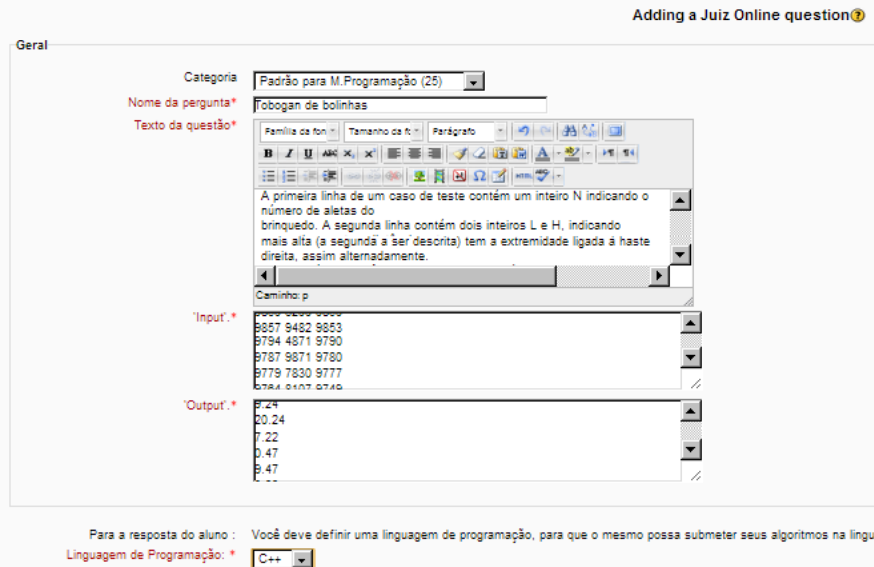
\includegraphics[scale=0.4]{pictures/BOCA_edicao.png}
        \fonte{\cite[p.~26]{galasso}}
\end{figure}

\begin{figure}[h!]
	   \centering
            \caption{Integração BOCA-Moodle - Visualização do retorno da avaliação da questão}
            \label{fig:ModeloConceitual}
	   	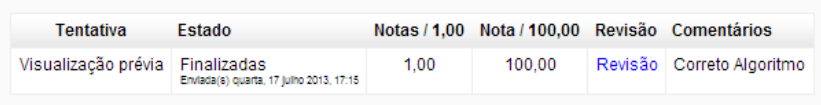
\includegraphics[scale=0.4]{pictures/BOCA_visualizacao.png}
        \fonte{\cite[p.~27]{galasso}}
\end{figure}

Para manter o desempenho do Moodle, a integração foi concebida de modo a garantir que os ambientes envolvidos fossem implementados em servidores independentes. Essa separação minimiza a possibilidade de sobrecarga no Moodle durante a avaliação dos algoritmos no BOCA. A integração foi desenvolvida com o PostgreSQL, e os bancos de dados do Moodle e do BOCA se comunicam via Dblink, um recurso que permite o acesso remoto a tabelas específicas.

As tabelas principais do BOCA envolvidas na avaliação automática incluem a “problemtable”, para cadastro de questões, “runtable”, para submissões dos alunos, “answertable”, para dados de correção, e “langtable”, com as linguagens de programação suportadas (C, C++ e Java). Os autores também criaram duas tabelas auxiliares, “tempaluno” e “tempprofessor”, para facilitar a transferência de dados entre o Moodle e o BOCA.

Os gatilhos (triggers) configurados no banco de dados são fundamentais para o fluxo de dados entre Moodle e BOCA, eliminando a necessidade de alterações no código. O fluxo começa quando o professor cadastra uma questão no Moodle, acionando gatilhos que transferem os dados para o BOCA, onde a questão é registrada. Da mesma forma, quando um aluno responde, gatilhos adicionais transferem as submissões para a tabela de execução no BOCA.

\begin{figure}[h!]
	   \centering
            \caption{Integração BOCA-Moodle - Fluxo da interação das bases de dados do Moodle e do BOCA}
            \label{fig:ModeloConceitual}
	   	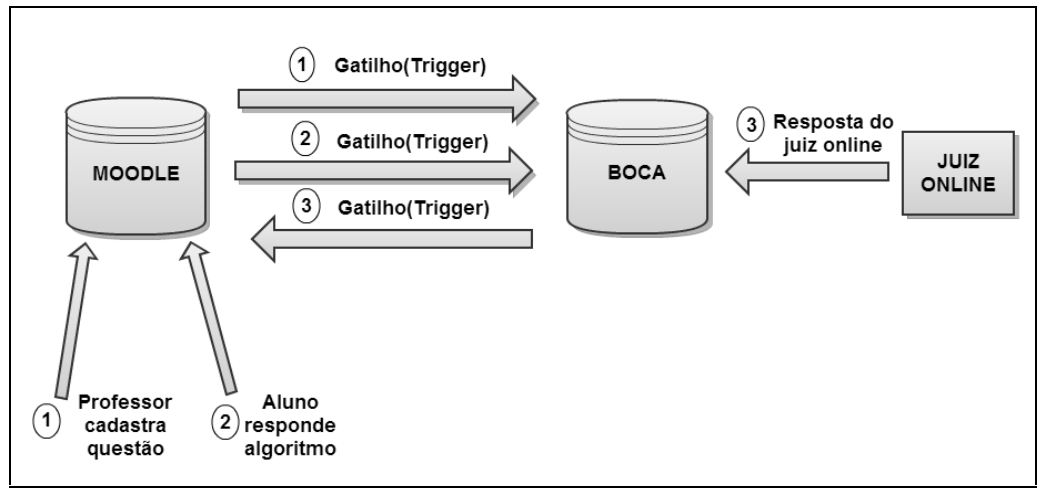
\includegraphics[scale=0.3]{pictures/BOCA_fluxo.png}
        \fonte{\cite[p.~29]{galasso}}
\end{figure}

Durante o julgamento das respostas, o BOCA executa scripts em intervalos de um minuto, verificando novas submissões e atualizando o status no Moodle. Os alunos visualizam uma área verde para respostas corretas e vermelha para incorretas. Figuras incluídas no estudo ilustram etapas do cadastro das questões e o \textit{feedback} visual ao aluno.

\begin{figure}[h!]
	   \centering
            \caption{Integração BOCA-Moodle - retorno da avaliação da questão como correta}
            \label{fig:ModeloConceitual}
	   	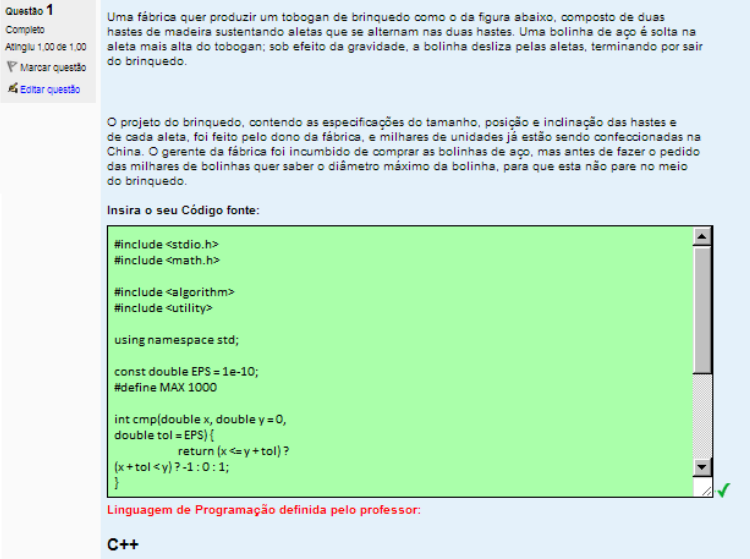
\includegraphics[scale=0.5]{pictures/BOCA_correta.png}
        \fonte{\cite[p.~26]{galasso}}
\end{figure}

Houve desafios técnicos, como a tentativa inicial de enviar arquivos “zip” diretamente para o banco de dados, o que levou a problemas de codificação. Para contornar isso, os arquivos foram transferidos via FTP, necessitando a instalação de um servidor FTP no ambiente do BOCA. Ao final, os autores ressaltam a importância de uma instalação simplificada e recomendam uma versão do BOCA já configurada para integração com o Moodle. Essa abordagem visa facilitar a adoção da solução e sua eficácia no ensino de algoritmos.

\section{CodeRunner: A Tool for Assessing Computer Programing Skills}

O estudo de \textcite{lobbharlow} examina as dificuldades encontradas na avaliação de alunos em disciplinas de programação utilizando métodos tradicionais, como provas de papel e caneta. O artigo destaca que a complexidade dos códigos e a natureza da programação moderna tornam a avaliação precisa um desafio, pois esses métodos não oferecem a possibilidade de realizar testes ou debug. O artigo propõe o uso de ferramentas de avaliação automatizadas, como o CodeRunner, que proporciona correção e \textit{feedback} imediato para os alunos.	

Pelo CodeRunner, plugin do Moodle, os alunos recebem um \textit{feedback} binário, onde as respostas corretas são indicadas por marcas verdes e as incorretas por cruzes vermelhas. A ferramenta adota o método de avaliação "tudo ou nada", ou seja, uma resposta só é considerada correta se atender completamente aos requisitos do teste, sendo a nota zero atribuída para respostas incorretas. Contudo, o sistema permite que os alunos façam múltiplas tentativas, oferecendo a chance de corrigir falhas como erros de compilação, formatação inadequada ou problemas de tempo de execução, com a possibilidade de aplicar penalidades em caso de envio tardio ou repetido.

\begin{figure}[h!]
	   \centering
            \caption{CodeRunner - A simples pergunta sobre Python, respondida erroneamente}
            \label{fig:ModeloConceitual}
	   	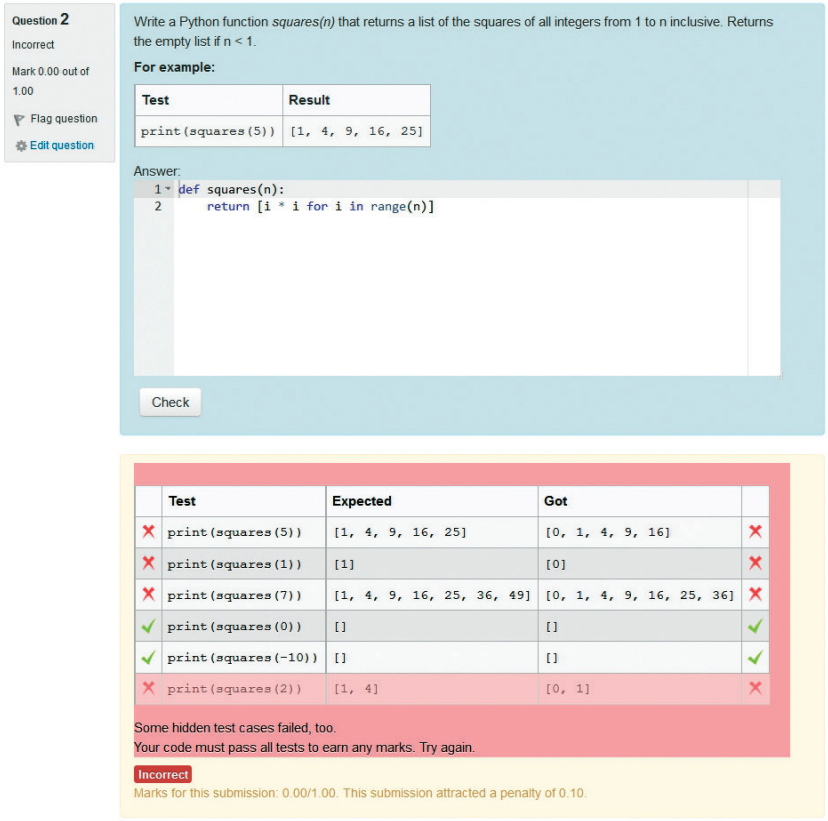
\includegraphics[scale=0.4]{pictures/CodeRunner_errada.png}
        \fonte{\cite[p.~48]{lobbharlow}}
\end{figure}

\begin{figure}[h!]
	   \centering
            \caption{CodeRunner - A simples pergunta sobre Python, respondida corretamente}
            \label{fig:ModeloConceitual}
	   	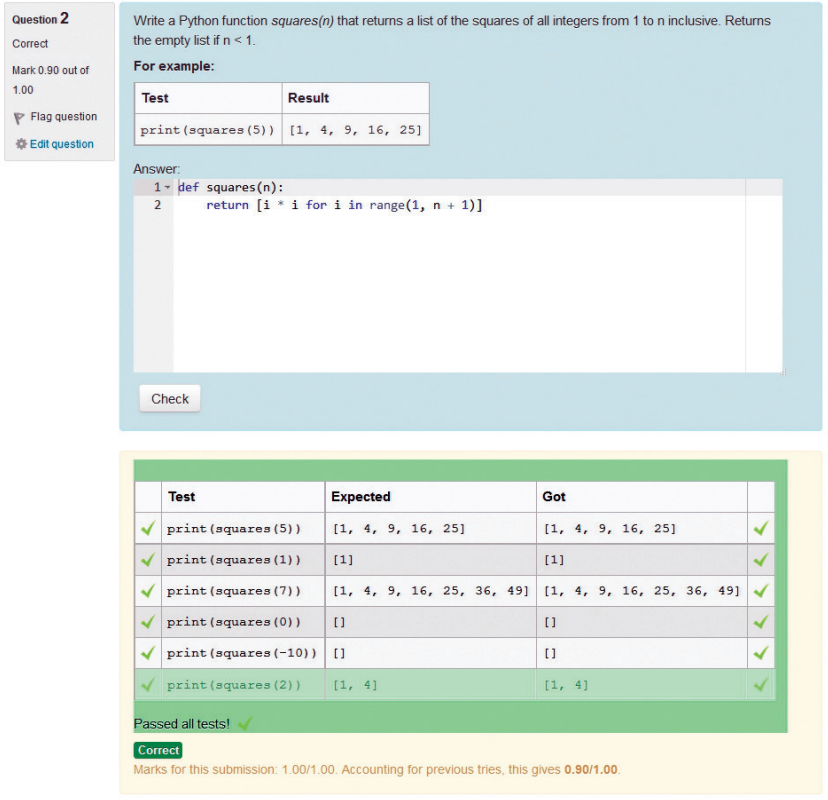
\includegraphics[scale=0.4]{pictures/CodeRunner_correta.png}
        \fonte{\cite[p.~48]{lobbharlow}}
\end{figure}

O CodeRunner também apresenta uma abordagem flexível para a criação de perguntas, permitindo que os desenvolvedores de questões criem protótipos personalizados. Esses protótipos podem ser usados para perguntas que exigem funcionalidades adicionais ou para impor restrições, como o uso de determinado tipo de estrutura de controle no código. Além disso, a execução do código do aluno ocorre em um ambiente seguro, isolado do servidor principal, o que evita riscos de segurança.

Apesar de o CodeRunner ter se revelado altamente eficaz em diversas atividades de avaliação, os autores destacaram algumas limitações fundamentais:

\begin{enumerate} [label=(\alph*)]
    \item O CodeRunner destaca-se em tarefas relativamente simples com especificações claras. Embora, teoricamente, qualquer pergunta com resposta mensurável por um programa de computador possa ser formulada como uma pergunta do CodeRunner, o esforço demandado para criar avaliadores para tarefas complexas muitas vezes inviabiliza essa abordagem, especialmente em turmas de maior tamanho;
    \item Ferramentas de qualidade de código, como o pylint, provaram ser muito valiosas para aumentar a conscientização sobre o estilo e melhorar a qualidade do código, mas ainda ocorrem abusos das regras de estilo, e a qualidade dos comentários e identificadores não pode ser avaliada por computador. Por isso, a avaliação humana ainda é reservada para a qualidade do código;
    \item A resposta a uma pergunta do CodeRunner deve ser apresentada como um único bloco de texto, predominantemente composto por código. Embora os autores das perguntas possam gerar diversos formatos de \textit{feedback}, inclusive gráficos, a apresentação padrão dos resultados é tabular, com uma linha para cada caso de teste e correspondência direta entre a saída esperada e a saída real. Caso os testes exijam blocos extensos de código ou resultem em saídas volumosas, a visualização dos resultados pode dificultar a compreensão pelos alunos do motivo pelo qual uma resposta foi marcada como incorreta;
    \item A avaliação de perguntas com resultados gráficos representa um desafio. Foi criado uma simulação do kit de ferramentas GUI tkinter em Python para avaliar interfaces gráficas na disciplina, incluindo perguntas que verificam a precisão de gráficos gerados por chamadas à biblioteca de gráficos do Matlab. Contudo, a avaliação da correção de imagens ou mesmo da saída de programas que envolvem gráficos complexos, como os da biblioteca de tartarugas, foi considerada uma tarefa difícil, senão impossível;
    \item Por último, é importante ressaltar que a elaboração de perguntas de qualidade e testes eficazes pode demandar considerável tempo, mesmo em cursos de programação de nível básico. O compartilhamento de bancos de dados de perguntas entre professores seria altamente benéfico nesse contexto.
\end{enumerate}


\section{A Virtual Programming Lab for Moodle with Automatic Assessment and Anti-Plagiarism Features}

\textcite{rodriguezdelpinoandroyo} descreveram neste artigo o módulo Virtual Programming Lab (VPL) para o Moodle, desenvolvido na Universidade de Las Palmas de Gran Canaria (ULPGC), e lançado para uso gratuito sob a licença GNU/GPL.

Para empregar uma linguagem de programação específica no VPL, basta garantir que o compilador correspondente esteja devidamente instalado no sistema de execução. Atualmente, estão disponíveis sistemas de execução com instalações para diversas linguagens, incluindo Ada, C, C\+\+, C\#, FORTRAN, Haskell, Java, Octave, Pascal, Perl, PHP, Prolog, Python, Ruby, Scheme, SQL e VHDL.
 
O VPL é composto por três elementos: um módulo do Moodle, um editor de código baseado em navegador e um componente Jail, mostrados na figura 16.

\begin{figure}[h!]
	   \centering
            \caption{VPL - Componentes}
            \label{fig:ModeloConceitual}
	   	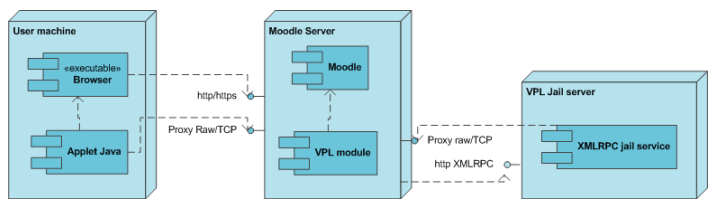
\includegraphics[scale=0.5]{pictures/VPL_componentes.png}
        \fonte{\cite[p.~2]{rodriguezdelpinoandroyo}}
\end{figure}

O editor de código, construído em Java, possibilita a edição, execução, depuração e avaliação de programas em um ambiente simples de desenvolvimento. Já o módulo do Moodle oferece características típicas, como backup, integração com o livro de notas e controle de eventos, além de recursos específicos, como gerenciamento de submissões, suporte à avaliação e prevenção contra plágio. E o componente Jail é um servidor que compila e executa códigos de alunos em um ambiente seguro, usando o comando linux chroot para restrições de leitura. 

O VPL permite configurar, gerenciar e avaliar atividades de aprendizagem, classificadas por tipo (exemplos, exercícios de cloze, exercícios de desenvolvimento de código) e escopo (tarefas fora da sala de aula ou exames em sala).

A criação de uma atividade VPL inicia-se com o preenchimento do formulário de configuração básica no Moodle, incluindo nome, descrição, período de disponibilidade, opções de avaliação e outras configurações. Além disso, é possível especificar detalhes como número máximo de arquivos, tamanho máximo, restrições de edição, rede e senha. Veja na imagem 18.

\begin{figure}[h!]
	   \centering
            \caption{VPL - Configuração básica de restrições}
            \label{fig:ModeloConceitual}
	   	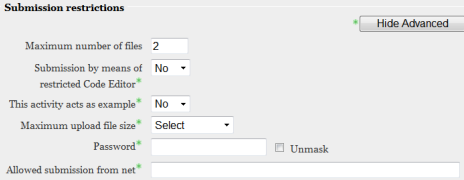
\includegraphics[scale=0.5]{pictures/VPL_config_basica.png}
        \fonte{\cite[p.~3]{rodriguezdelpinoandroyo}}
\end{figure}

Após preencher o formulário básico, o instrutor pode ajustar cinco grupos adicionais de recursos na ferramenta VPL. A guia "Descrição completa" permite fornecer detalhes sobre o problema a ser resolvido. Em "Casos de teste", é possível configurar testes com descrição, entrada, saída esperada e penalizações em caso de falha. A guia "Options" configura aspectos gerais, como a base da atividade, permissões dos alunos e se os resultados automáticos contam para a nota final. "Arquivos solicitados" determina os nomes obrigatórios dos arquivos a serem enviados. 

Essas configurações são suficientes, mas a guia "Advanced" oferece recursos adicionais para testes mais elaborados, como testes de funcionalidade avançados e outros tipos de teste, possibilitando uma avaliação abrangente da qualidade do código.

A figura 19 mostra um exemplo de configuração de casos de teste, e a figura 20 mostra a tela de configuração de casos de teste mais avançados.

\begin{figure}[h!]
	   \centering
            \caption{VPL - Exemplo de configuração de casos de teste}
            \label{fig:ModeloConceitual}
	   	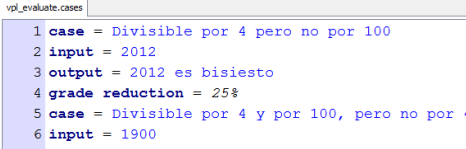
\includegraphics[scale=0.5]{pictures/VPL_testes.png}
        \fonte{\cite[p.~3]{rodriguezdelpinoandroyo}}
\end{figure}

\begin{figure}[h!]
	   \centering
            \caption{VPL - Arquivos de execução para testes avançados}
            \label{fig:ModeloConceitual}
	   	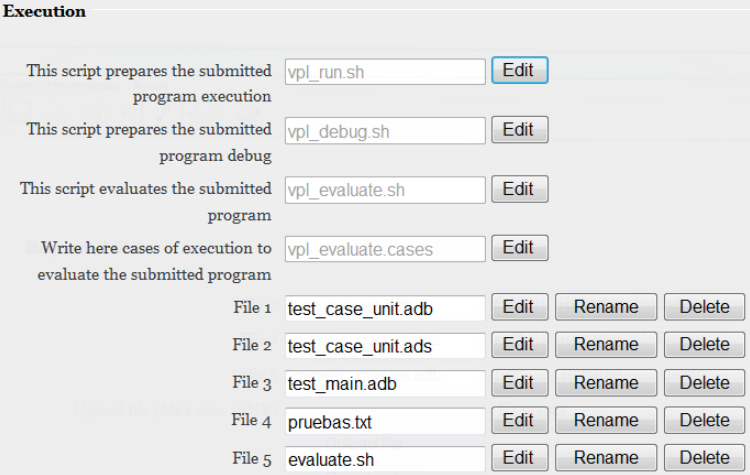
\includegraphics[scale=0.5]{pictures/VPL_testes_avancados.png}
        \fonte{\cite[p.~4]{rodriguezdelpinoandroyo}}
\end{figure}

O VPL oferece avaliação automática e assistida por computador, permitindo a personalização através das opções na guia correspondente. É essencial configurar os testes para respaldar a avaliação. O VPL realiza automaticamente os testes configurados, fornecendo um relatório com testes falhos, comentários explicativos e uma proposta de nota. O avaliador humano tem a flexibilidade de ajustar o relatório, excluindo ou adicionando comentários, reutilizando itens da lista e recalculando a nota conforme necessário.

O plágio é abordado pelo VPL através de uma ferramenta de verificação de plágio no código-fonte. Essa ferramenta procura identificar plágio entre os envios de uma tarefa em um curso, considerando também fontes como envios anteriores ou tarefas similares de outros cursos. O processo de identificação de semelhanças entre os arquivos de origem envolve três etapas: tokenização, comparação e clusterização. 

A tokenização visa obter uma assinatura normalizada para facilitar a comparação eficiente, envolvendo análise lexical, filtragem e normalização. Esse processo cria uma assinatura do programa, que é uma representação normalizada dos arquivos de código-fonte de um usuário, otimizando o processo de comparação, permitindo a detecção eficaz de plágio.

Em resumo, o Virtual Programming Lab (VPL) apresenta-se como uma ferramenta abrangente para o gerenciamento de atividades de programação. Com recursos que vão desde a configuração detalhada de atividades no Moodle até a execução de testes avançados e a detecção de plágio, o VPL oferece uma variedade de funcionalidades para apoiar a aprendizagem prática e avaliação de habilidades de programação. Destaca-se, além disso, a necessidade de configurar todos os exercícios e seus casos de teste, para disponibilização destes aos alunos.


\section{Uma Ferramenta Baseada em Juízes Online para o Apoio às Atividades de Programação de Computadores no Moodle}

No projeto conduzido por \textcite{joseosvaldochaves}, foi desenvolvido o Módulo de Integração com Juízes Online (MOJO), ferramenta que integra os Juízes Online, como o Timus Online Judge e o Beecrowd (conhecido como URI Online Judge na época) ao Moodle, para evitar que os professores de disciplinas de programação ficassem sobrecarregados ao ter que elaborar, submeter, abaliar e fornecer o \textit{feedback} necessário das questões aos alunos. O MOJO automatizou o processo de Elaboração, Submissão e Avaliação (ESA) das atividades de programação, fornecendo um ambiente unificado que facilita o acompanhamento dos alunos e amplia o acesso a um maior número de questões.

O MOJO, portanto, integra o Moodle com os Juízes Online para atividades de programação, sem interação direta entre as plataformas. Ele automatiza o processo ESA (Elaboração, Submissão e Avaliação), permitindo que professores submetam questões no Moodle, estudantes enviem suas respostas, e os Juízes Online avaliem automaticamente o código, com os resultados retornando ao Moodle para análise de professores e alunos. O professor pode monitorar o progresso dos estudantes e acessar os códigos submetidos, enquanto o Repositório de Integração armazena as questões para uso futuro.

Na arquitetura geral do MOJO, o Moodle gerencia a interface e o controle das atividades de programação, enquanto o MOJO se encarrega da comunicação e interação com os Juízes Online. A arquitetura conta com o Módulo Principal (MOP), responsável pelas funcionalidades essenciais e pelo controle do Módulo de Carga e Atualização (MOCA), que, por sua vez, realiza o carregamento inicial e atualizações constantes das questões, armazenando-as no Repositório de Integração. Esse repositório mantém as questões e resultados para uso e acompanhamento contínuo no Moodle.

Como os juízes online não oferecem APIs ou serviços Web, foram necessárias implementações específicas para cada juiz, utilizando PHP (a mesma linguagem do Moodle) e JavaScript para a interface. O banco de dados PostgreSQL foi escolhido por ser open-source e por permitir a criação de tabelas personalizadas para armazenar dados dos alunos, viabilizando um \textit{feedback} direcionado e adequado.

O objetivo do MOJO é reduzir a carga de trabalho dos professores no processo ESA, permitindo um acompanhamento mais próximo dos alunos. Em uma pesquisa inicial com sete professores, os resultados apontaram que 71,4\% acreditam que a ferramenta pode economizar tempo; 28,6\% gostariam de poder criar e avaliar suas próprias atividades automaticamente; 42,8\% mencionaram questões de legibilidade do código; 28,6\% observaram a clareza dos resultados; 85,7\% valorizam o feedback mais rápido aos alunos; e 100\% acreditam que a redução de tarefas possibilitará um acompanhamento mais eficaz, especialmente para alunos com dificuldades.


\section{Building of a Rule-Based Expert System for Academic Advising via Web Expert System Tools}

O projeto conduzido por \textcite{osmannasr} aborda o desenvolvimento de um sistema especialista voltado para otimizar o aconselhamento acadêmico na Universidade King Khalid. A proposta central do estudo é criar uma ferramenta que simule as funções do conselheiro acadêmico humano, utilizando técnicas de inteligência empresarial para auxiliar na tomada de decisões informadas por estudantes e funcionários, baseadas nas regulamentações acadêmicas da instituição.

O processo de desenvolvimento do sistema é dividido em várias fases, cada uma com objetivos específicos:

Fase de Análise: Esta etapa inicial é dedicada à coleta de informações sobre as questões mais recorrentes entre os estudantes, além de procedimentos acadêmicos frequentes, como matrícula em cursos, transferências de departamento e pedidos de suspensão. A análise dessas necessidades foi realizada por meio de entrevistas com estudantes e conselheiros acadêmicos, utilizando uma abordagem de árvore de decisão (UML), mostrada na Figura 20, para entender melhor os requisitos do sistema.

\begin{figure}[h!]
        \centering
         \caption{Sistema especialista baseado em regras - Árvore de decisão}
         \label{fig:ModeloConceitual}
                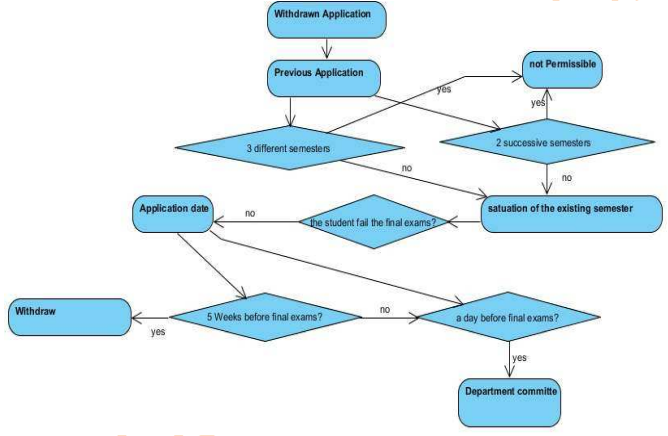
\includegraphics[scale=0.5]{pictures/Rule_Based_Expert_System_arvore_decisao.png}
     \fonte{\cite[p.~305]{neildunstan}}
\end{figure}

Fase de Design: Com base na análise anterior, o design do sistema foi estruturado utilizando uma metodologia baseada em regras (rule-based). Esse método foi escolhido por sua adequação à modelagem dos processos de aconselhamento acadêmico, que envolvem uma lógica condicional do tipo "se-então". Durante essa fase, também foi projetada uma interface amigável, alinhada com o estilo visual e os padrões de interação do portal da universidade, garantindo que os usuários pudessem facilmente se adaptar ao sistema.

Fase de Implementação: A construção do sistema foi realizada utilizando o ES Builder, uma ferramenta de código aberto que facilita a criação de sistemas especialistas baseados em regras. O sistema foi projetado para ser acessível via plataforma web, o que possibilita seu uso por uma grande variedade de usuários, incluindo estudantes e conselheiros acadêmicos.

Fase de Testes e Avaliação: O sistema foi testado com diferentes cenários, utilizando tanto estudantes quanto conselheiros acadêmicos, a fim de validar sua eficácia. Os resultados indicaram que o sistema é capaz de fornecer respostas adequadas e de auxiliar no processo de aconselhamento de forma precisa e eficiente.

O estudo conclui que a implementação de sistemas especialistas no âmbito acadêmico tem um grande potencial para melhorar a eficiência do aconselhamento acadêmico, promovendo uma interação mais eficaz entre estudantes e conselheiros. Além disso, o sistema proposto pode se tornar uma ferramenta valiosa para a tomada de decisões informadas, não apenas para os estudantes, mas também para os docentes, que poderão fornecer orientações mais precisas e baseadas em dados. O sistema mostrou-se alinhado às expectativas dos usuários, que manifestaram interesse em expandir sua funcionalidade para cobrir mais áreas do aconselhamento acadêmico.

Este trabalho evidencia o papel transformador que a tecnologia pode desempenhar no setor educacional, especialmente no contexto do aconselhamento acadêmico, apontando para a necessidade de continuar a pesquisa e o desenvolvimento de sistemas dessa natureza para atender de forma mais abrangente às necessidades dos estudantes e professores.


\section{An Interactive Web-Based Expert System Degree Planner}

O artigo desenvolvido por \textcite{neildunstan} descreve o desenvolvimento de um planejador de grau acadêmico baseado na web (seu layout é mostrado na Figura 21), utilizando XML (Extensible Markup Language) e sistemas especialistas. O sistema possui um servidor que hospeda arquivos XML para cada grau acadêmico, descrevendo unidades e regras associadas. Essas regras são importadas para uma interface web genérica, permitindo a personalização do visual com uma paleta de unidades e horários disponíveis para os semestres. As regras do grau acadêmico em formato XML são convertidas em código Prolog, que permite ao sistema responder a consultas complexas relacionadas ao planejamento de cursos.

\begin{figure}[h!]
        \centering
         \caption{Planejador de grau acadêmico - Layout da página}
         \label{fig:ModeloConceitual}
                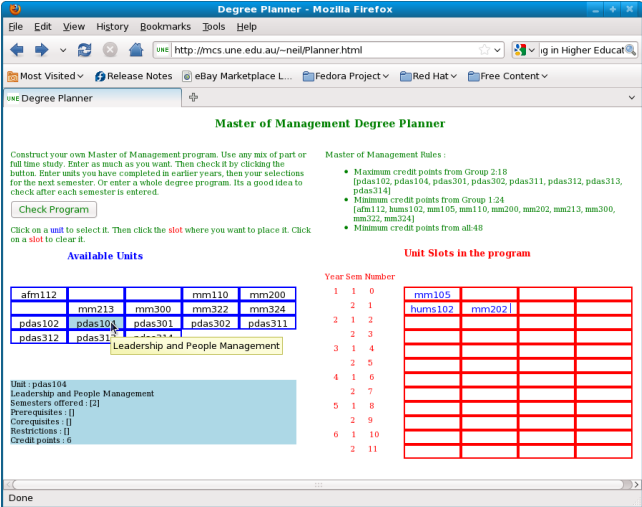
\includegraphics[scale=0.5]{pictures/degree_planner_page_layout.png}
     \fonte{\cite[p.~305]{neildunstan}}
\end{figure}

O design do sistema é baseado na separação clara entre o tratamento da interface do usuário no cliente e o processamento de regras no servidor (Figura 22). O servidor utiliza um sistema especialista em Prolog para resolver consultas mais complexas, enquanto o cliente lida com informações mais simples por meio de JavaScript. O sistema é acessível via navegador e não requer plugins específicos, sendo adequado para dispositivos móveis, como smartphones.

\begin{figure}[h!]
        \centering
         \caption{Planejador de grau acadêmico - Interação cliente-servidor}
         \label{fig:ModeloConceitual}
                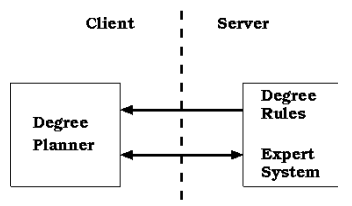
\includegraphics[scale=0.5]{pictures/degree_planner_client_server.png}
     \fonte{\cite[p.~304]{neildunstan}}
\end{figure}

A interface do usuário é composta por várias seções, incluindo uma paleta de unidades, um cronograma de programa semestral e um painel de exibição de detalhes das unidades selecionadas. Os estudantes podem explorar opções de inscrição e verificar se suas escolhas atendem aos requisitos do curso. O sistema permite que os alunos ajustem seu programa acadêmico, respondendo a perguntas sobre requisitos de unidades e pré-requisitos, de forma interativa e personalizada.

Conclui-se que o uso de sistemas especialistas em planejadores de grau acadêmico baseados na web pode melhorar a interatividade e fornecer orientações mais precisas aos alunos, ajudando-os a construir um programa de graduação adequado aos seus interesses e cronograma, sem a necessidade de plugins ou instalações específicas.


\section{Comparação entre os Trabalhos}

O estudo de \cite{cruz2022} ressalta a eficácia da integração da plataforma Beecrowd em um plano de ensino inovador para disciplinas de programação. Ao incorporar estratégias como sala de aula invertida e gamificação, a pesquisa conclui que o Beecrowd, utilizado como suporte para a gamificação, não só melhora o processo de ensino e aprendizagem, oferecendo suporte aos educadores e motivando os alunos, mas também contribui para a redução da evasão em cursos superiores de informática.

A aplicação das metodologias propostas no estudo dos autores demonstrou um impacto significativo no desempenho dos alunos ao longo do tempo na universidade dos autores, resultando em um crescimento notável e consistente nas notas. A ferramenta Beecrowd, destacada no estudo, é elogiada pela sua organização meticulosa de desafios em categorias e níveis de dificuldade, além de sua abordagem de maratona de programação, revelando-se eficaz em envolver os alunos de maneira imersiva.

A Tabela 1 apresenta uma comparação detalhada das vantagens do Beecrowd em relação a outras ferramentas integradas ao Moodle, como BOCA, VPL e CodeRunner, conforme discutido nos trabalhos relacionados. O objetivo é analisar os benefícios específicos do uso do Beecrowd, oferecendo uma base sólida para este estudo. Vale ressaltar que este trabalho propõe o incentivo ao uso da integração entre Moodle e Beecrowd por meio de LTI. Em contraste, o BOCA e o CodeRunner funcionam como tipos de questões no Moodle, enquanto o VPL é um módulo próprio da plataforma.

\begin{table}[htb]
        \IBGEtab{%
          \caption[Comparação entre quatro integrações de sistemas, que auxiliam no ensino da programação, com o Moodle: Beecrowd, BOCA, CodeRunner e VPL]{Comparação entre quatro integrações de sistemas, que auxiliam no ensino da programação, com o Moodle: Beecrowd, BOCA, CodeRunner e VPL}%
          \label{tabela-ibge}
        }{%
          \begin{tabular}{c c c c c}
          \toprule
           \textbf{Aspecto} & \textbf{Beecrowd} & \textbf{BOCA} & \textbf{VPL} & \textbf{CodeRunner} \\
          \midrule
          Possui Juiz Online	                        &  X	& X	& X	& X   \\ \midrule
          Fornece \textit{feedback} Imediato	                &  X	& X	& X	& X   \\ \midrule
          Criação Manual de Questões	                &  	& X	& X	& X   \\ \midrule
          Questões Prontas para Professores	        &  X	& 	& 	&    \\ \midrule
          Questões Prontas classificadas por categoria  &  X	& 	& 	&    \\ \midrule
          Inserção Manual de Casos de Teste	        &  	& X	& X	& X   \\ \midrule
          Suporta Diversas Linguagens	                &  X	& X	& X	& X   \\ \midrule
          Pré-processamento de Submissões	        &  	& 	& 	& X   \\ \midrule
          Comentários de Testes Falhados	        &  	& 	& X	&    \\ \midrule
          Prevenção de Plágio	                        &  X	& 	& X	&    \\ \midrule
          Incentiva participar de maratonas de programação    &  X	& 	& 	&    \\ 
          \bottomrule
        \end{tabular}%
        }{%
          \fonte{
              Produzido pela autora. 
          }%
        }
      \end{table}

A análise da tabela destaca o Beecrowd como notavelmente diferenciado em relação aos outros sistemas, sobretudo devido à presença de questões pré-existentes para os professores. Essa característica elimina a necessidade de cadastramento manual das questões de programação e seus respectivos testes, uma exigência presente nas plataformas BOCA, VPL e CodeRunner. Como confirmação, uma das limitações do CodeRunner apontadas por \textcite{lobbharlow} é o fato de a criação de perguntas e testes de qualidade demandar tempo, além de ser mais adequado para tarefas simples e bem definidas, já que a criação de testes para atividades complexas exige muito esforço, especialmente em turmas grandes.

Um aspecto distintivo e relevante nos sistemas BOCA, VPL e CodeRunner é a abordagem de desenvolvimento que incorpora a utilização de servidores separados para o Moodle e os sistemas juízes online. Essa estratégia visa garantir a execução independente e eficiente de cada componente, proporcionando benefícios tanto em termos de desempenho quanto de segurança.

A adoção de servidores separados para o Moodle e os sistemas juízes online tem como objetivo otimizar a distribuição de carga, prevenindo sobrecargas e garantindo uma operação mais estável e responsiva. Essa separação também fortalece a segurança, pois ao isolar cada plataforma, diminui-se os riscos de conflitos e vulnerabilidades. Da mesma forma, ela possibilita uma escalabilidade mais eficiente, permitindo que cada sistema seja dimensionado conforme suas necessidades específicas, sem afetar o desempenho do outro. Isso é particularmente importante em ambientes acadêmicos, onde a demanda por plataformas e sistemas pode variar significativamente.

O trabalho de \textcite{rodriguezdelpinoandroyo} mostra que o módulo Virtual Programming Lab (VPL) possui um editor de código em Java para editar, executar, depurar e avaliar programas em um ambiente simples de desenvolvimento. Dessa forma, para utilizar todas as funcionalidades é necessário um navegador com suporte a JavaScript e applets Java. Já os trabalhos de \textcite{lobbharlow} e \textcite{galasso} mostram que tanto o CodeRunner quanto o BOCA disponibilizam caixas de texto nas quais os usuários podem escrever ou colar o código, permitindo sua subsequente avaliação.

Neste trabalho, a integração LTI fornecida pelo Beecrowd será utilizada, de modo que a criação de listas de exercícios, a resolução de exercícios pelos alunos e a correção das soluções pelo juiz online ocorrerão diretamente nos servidores do Beecrowd.

Além disso, a prevenção contra plágio é uma característica crucial e distintiva tanto no Beecrowd quanto no VPL, destacando-se como um diferencial significativo dessas plataformas. Essa funcionalidade visa salvaguardar a integridade acadêmica, garantindo que os trabalhos submetidos pelos alunos sejam autênticos e originais.

No contexto do Beecrowd, de acordo com \cite{cruz2022}, a prevenção contra plágio pode envolver mecanismos avançados de análise de código-fonte, identificando padrões suspeitos que indicam possível cópia indevida. Além disso, o sistema pode empregar algoritmos e técnicas que comparam soluções de diferentes alunos, buscando similaridades que ultrapassem limites aceitáveis de coincidência.

No caso do VPL, de acordo com \textcite{rodriguezdelpinoandroyo}, a prevenção contra plágio pode ser implementada através de verificações rigorosas durante o processo de submissão. Isso pode incluir a comparação automática de códigos submetidos em busca de trechos idênticos ou substancialmente semelhantes. Além disso, o VPL pode adotar métodos de análise mais avançados, como a detecção de técnicas de programação específicas que são características de trabalhos plagiados.

O projeto de \textcite{joseosvaldochaves} descreve o desenvolvimento do Módulo de Integração com Juízes Online (MOJO), uma ferramenta criada para integrar juízes online, como o Beecrowd (anteriormente URI Online Judge), ao Moodle. O MOJO visa delegar ao Moodle o gerenciamento da interface e do controle das atividades de programação, enquanto centraliza a comunicação e interação com os juízes online. Devido à ausência de APIs ou serviços web nos juízes à época, foram necessárias implementações específicas para cada plataforma, utilizando PHP (a mesma linguagem do Moodle) e JavaScript para a interface. O banco de dados PostgreSQL foi adotado por ser open-source e pela flexibilidade de criação de tabelas personalizadas para armazenamento de dados dos alunos, o que possibilita um \textit{feedback} direcionado e preciso.

Este trabalho, contudo, utilizará a integração LTI fornecida pelo Beecrowd, a qual facilita a interação de docentes e alunos com a plataforma. Além disso, será disponibilizado um manual para orientar o uso da LTI, juntamente com um sistema especialista que auxiliará os alunos na resolução das questões e os docentes no esclarecimento de dúvidas dos estudantes.

É relevante notar que 100\% dos professores entrevistados para avaliar a eficácia do MOJO acreditam que a redução de tarefas permitirá um acompanhamento mais eficaz dos estudantes, especialmente daqueles que apresentam maiores dificuldades.

Por fim, os projetos de \textcite{osmannasr} e \textcite{neildunstan} abordam a construção de sistemas especialistas para o aconselhamento e planejamento acadêmico, porém apresentam enfoques e abordagens técnicas distintas.

No primeiro trabalho, \textcite{osmannasr} desenvolve um sistema especialista baseado em regras para o aconselhamento acadêmico na Universidade King Khalid. Este sistema é focado em replicar o processo de tomada de decisão dos conselheiros acadêmicos humanos, utilizando uma metodologia de árvore de decisão, implementada através do ES Builder, uma ferramenta de código aberto para sistemas especialistas baseados em regras, com uma interface web simples e uma lógica de "se-então". Essa escolha reflete a necessidade de simular de forma prática e direta o trabalho dos conselheiros humanos sem uma complexidade computacional elevada.

No segundo trabalho, \textcite{neildunstan} foca em um planejador de grau acadêmico, utilizando uma abordagem híbrida com XML e Prolog para gerenciar e responder a consultas complexas. As regras para cada programa acadêmico são estruturadas em XML e convertidas em Prolog, possibilitando que o sistema lide com consultas interativas e personalizadas. A arquitetura desse sistema é distribuída, com o cliente manipulando a interface e o servidor processando as regras em Prolog. Essa separação facilita o uso em dispositivos móveis e oferece flexibilidade ao permitir que os alunos construam e verifiquem seu programa acadêmico de maneira independente e intuitiva, sem plugins específicos.

Já neste trabalho, será utilizado o Prolog como servidor da aplicação, responsável pelo gerenciamento de requisições HTTP, armazenamento de dados de sessão e comunicação contínua com o front-end. O servidor proporcionará um ambiente dinâmico para o carregamento modular de arquivos específicos de cada questão, permitindo a adaptação das perguntas e a personalização das respostas conforme as interações do usuário. Além disso, configurará permissões de CORS para integrar facilmente com a interface web, que será desenvolvida utilizando o React, uma biblioteca JavaScript para construção de interfaces de usuário interativas e reativas.

\end{otherlanguage*}

    % Primeiro capitulo de Resultados
    
% The \phantomsection command is needed to create a link to a place in the document that is not a
% figure, equation, table, section, subsection, chapter, etc.
% https://tex.stackexchange.com/questions/44088/when-do-i-need-to-invoke-phantomsection
\phantomsection

% Multiple-language document - babel - selectlanguage vs begin/end{otherlanguage}
% https://tex.stackexchange.com/questions/36526/multiple-language-document-babel-selectlanguage-vs-begin-endotherlanguage
\begin{otherlanguage*}{brazil}

\chapter{Desenvolvimento}

Nesta seção, será abordada a LTI do Beecrowd, que simplifica a integração entre o Moodle e a plataforma Beecrowd. Serão apresentados também os detalhes da implementação da aplicação web do sistema especialista, desenvolvida para auxiliar professores e alunos no esclarecimento de dúvidas recorrentes sobre as questões do Beecrowd, facilitando a adaptação de ambos ao uso da plataforma.

\section{LTI Beecrowd}

Com a disponibilização de uma ferramenta LTI pelo Beecrowd, visando facilitar sua integração com o Moodle, foi elaborado um manual detalhado para orientar o administrador do Moodle na configuração dessa LTI (Apêndice A).

Para configurar uma LTI externa, o administrador deve acessar "Administração do site", selecionar "Plugins" e, em "Módulos de atividade", escolher "Ferramenta externa" e clicar em "Gerenciar ferramentas". Em seguida, deve clicar em "Configurar uma ferramenta manualmente" e preencher os campos conforme as instruções especificadas no Manual de Configuração da LTI Beecrowd no Moodle (Apêndice A). Após a configuração, será possível visualizar os detalhes da ferramenta, os quais deverão ser enviados ao Beecrowd para estabelecer a comunicação entre as plataformas.

Além disso, foi desenvolvido um manual de uso da LTI Beecrowd (Apêndice B), direcionado aos professores que desejam utilizar o Beecrowd como suporte educacional em sala de aula. Esse manual instrui os docentes sobre como criar uma atividade do Beecrowd no Moodle, orientar o acesso dos estudantes e transferir as notas obtidas no Beecrowd para o Moodle.

Após seguir o guia do Manual de Uso da LTI Beecrowd (Apêndice B), duas atividades ficam disponíveis na página do curso, apresentadas como "botões" visuais. A primeira atividade, que é ocultada para os estudantes (Imagem 23), permite ao professor acessar o Beecrowd Academic (Imagem 24) para configurar disciplinas, criar listas de exercícios para os alunos e enviar as notas para o Moodle.

\begin{figure}[H]
    \centering
            \caption{Atividade para o professor acessar o Beecrowd Academic}
            \label{fig:ModeloConceitual}
        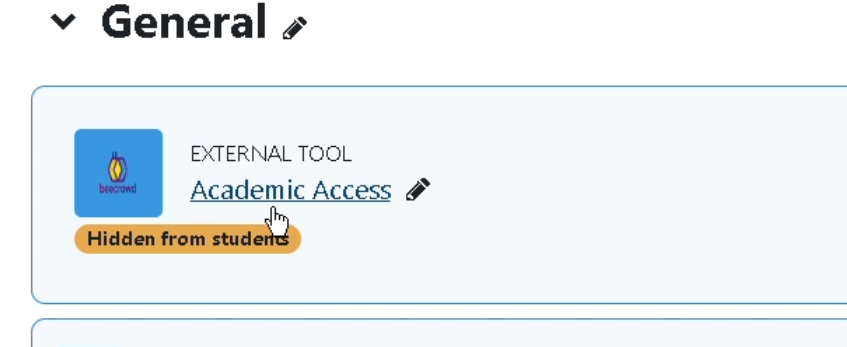
\includegraphics[scale=0.35]{pictures/apendices/apendice_b_5.png}
        \fonte{Produzido pela autora.}
\end{figure}

\begin{figure}[H]
    \centering
            \caption{Beecrowd Academic}
            \label{fig:ModeloConceitual}
        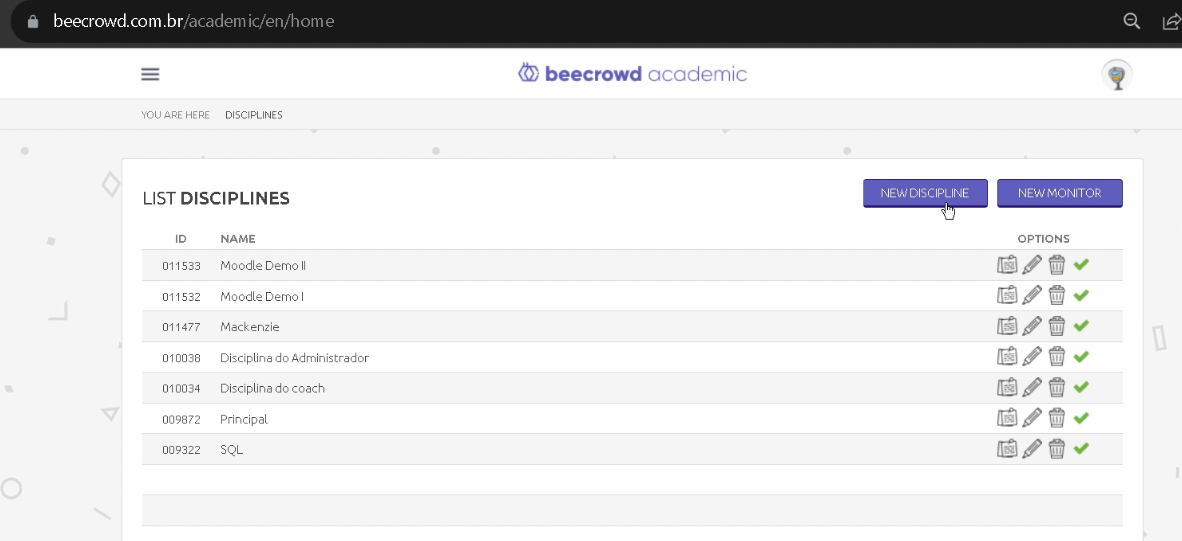
\includegraphics[scale=0.38]{pictures/desenvolvimento/lti_beecrowd_academic.png}
        \fonte{Produzido pela autora.}
\end{figure}

A segunda atividade, acessível aos estudantes (Imagem 25), redireciona-os diretamente para a página no Beecrowd da lista de exercícios criada pelo professor (Imagem 26), sem necessidade de cadastro ou login. Assim, os estudantes podem resolver as atividades diretamente a partir dessa página. Esse botão também permite ao professor acessar a lista de exercícios criada, podendo verificar o progresso dos alunos, as tentativas realizadas e, quando desejado, enviar as notas para o Moodle.

\begin{figure}[H]
    \centering
            \caption{Atividade para o aluno acessar o Beecrowd}
            \label{fig:ModeloConceitual}
        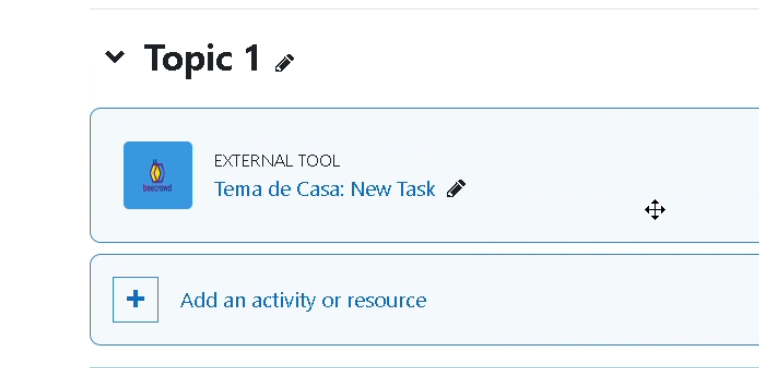
\includegraphics[scale=0.4]{pictures/desenvolvimento/lti_tarefa.png}
        \fonte{Produzido pela autora.}
\end{figure}

\begin{figure}[H]
    \centering
            \caption{Beecrowd do aluno}
            \label{fig:ModeloConceitual}
        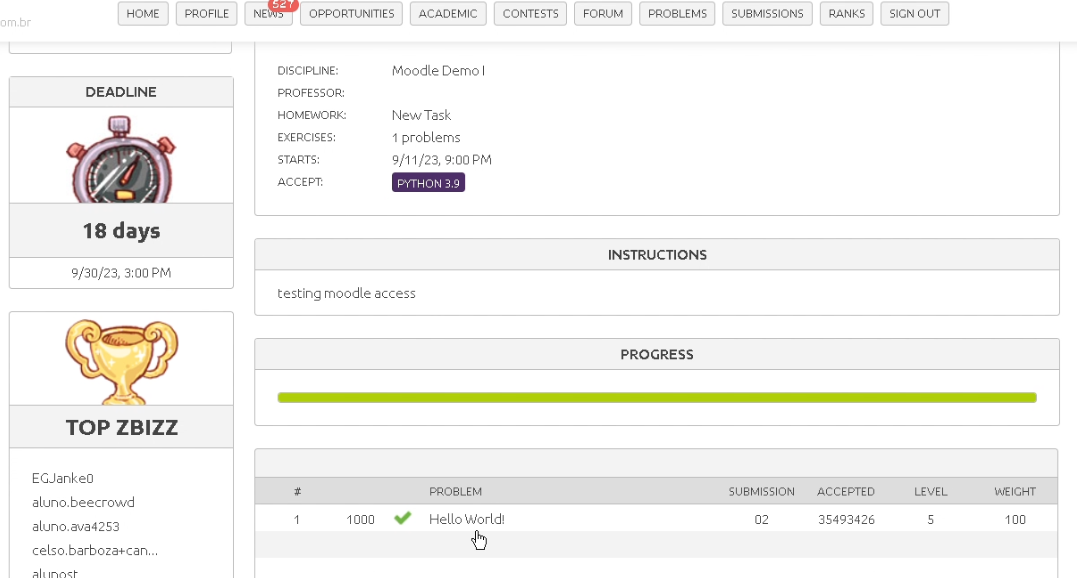
\includegraphics[scale=0.4]{pictures/desenvolvimento/lti_beecrowd_aluno.png}
        \fonte{Produzido pela autora.}
\end{figure}

\section{Sistema Especialista Web}

O objetivo do sistema especialista é oferecer suporte na resolução de dúvidas recorrentes dos estudantes em relação a questões do Beecrowd. A proposta é desenvolver uma aplicação acessível aos alunos via navegador, com um sistema de chat onde o aluno pode informar a questão sobre a qual necessita orientação. O sistema, então, conduz o aluno por meio de perguntas binárias (sim ou não) e, conforme as respostas, fornece dicas relevantes relacionadas ao exercício em questão.

Para viabilizar essa funcionalidade, o sistema especialista será estruturado com um conjunto de dados contendo perguntas direcionadas aos alunos e respostas predefinidas que orientam o aluno na resolução das atividades específicas da disciplina. Em disciplinas como Programação Orientada a Objetos I, onde as listas de exercícios frequentemente incluem questões já utilizadas em semestres anteriores, observa-se uma repetição de problemas e, consequentemente, de dúvidas recorrentes dos alunos.

Assim, a primeira etapa deste trabalho consistiu na coleta de dados sobre as questões, visando identificar e catalogar as dúvidas mais comuns.

\subsection{Coleta de Dados}

Nesta fase, foram realizadas duas coletas de dados: uma com dicas de resolução fornecidas pelo professor para uma lista de exercícios, e outra com as dúvidas dos alunos sobre o uso de listas em Python, com foco em questões específicas.

Na primeira coleta, professor da disciplina de Programação Orientada a Objetos I, da Universidade Federal de Santa Catarina (UFSC), forneceu dicas de resoluções para cada questão de uma lista de exercícios que ainda não tinha sido repassada aos alunos, com o objetivo de avaliar a utilidade da aplicação após ela ser desenvolvida. Assim, quando os alunos fossem resolver a lista de exercícios, poderiam testar a aplicação para ser sua eficácia. As questões abordadas, que receberam as dicas de solução, incluem: 1261, 1281, 1430, 1449, 1483, 1763, 1991, 1953, 2091, 2482, 2492, 2654, 2949 e 2987.

Na segunda coleta, foram registradas as dúvidas dos alunos da disciplina de Programação Orientada a Objetos I, da UFSC, coletadas no dia 30 de outubro de 2024. Nessa data, os alunos estavam trabalhando em uma lista de exercícios sobre o uso de listas em Python. As questões abordadas incluíram os problemas de números 1187, 1435, 1715, 2436, 1383, 1184, 1181 e 1185. Um aspecto notável foi que, durante essa mesma aula, quatro alunos apresentaram a mesma dúvida em relação à questão 1435, especificamente perguntando: "Como resolvo essa questão?"

Durante as 2h30 de aula, a questão 1435 foi a que suscitou o maior número de dúvidas entre os estudantes. Em uma turma de 26 alunos – embora nem todos tenham alcançado essa questão no tempo da aula –, quatro solicitaram uma explicação geral sobre a abordagem para resolvê-la, enquanto dois buscaram orientação sobre a conversão dessa abordagem para o código. Adicionalmente, três alunos enfrentaram o erro "Presentation Error" e um aluno recebeu o erro "Run-time Error".

As dúvidas em relação à questão 1181 refletiram dificuldades comuns no uso de laços de repetição e na manipulação de matrizes. Muitos estudantes não obtinham a resposta correta, mesmo com uma solução aparentemente desenvolvida, devido à confusão na seleção dos elementos da matriz, com erros ao iterar pelas linhas em vez das colunas. Os alunos também enfrentaram dificuldades na estruturação do laço de repetição, especialmente ao calcular a soma dos elementos de uma linha específica e ao determinar o divisor correto para o cálculo da média. Problemas de formatação, que resultaram no erro "Presentation Error", também foram recorrentes, sendo necessário ajustar a saída para uma casa decimal com '%.1f'.

Na questão 1184, as dificuldades estavam relacionadas à estruturação do laço de repetição para percorrer corretamente os elementos abaixo da diagonal principal da matriz. Os alunos foram orientados a usar um laço duplo, com a sequência correta de for i in range(0, 12) e for j in range(0, i). Além disso, houve dúvidas sobre a exclusão dos elementos da diagonal principal, que não deveriam ser somados. Como na questão 1181, os alunos enfrentaram dificuldades de formatação, com orientações para ajustar a saída utilizando '%.1f' para obter uma casa decimal.

As dúvidas relativas à questão 1185 envolveram a manipulação de elementos acima da diagonal secundária da matriz, com os alunos sendo orientados a percorrer as linhas até o último índice da coluna, subtraindo o número da linha. A configuração correta dos laços de repetição foi outra dúvida comum, com muitos alunos invertendo os laços, o que afetou os resultados. A correção do divisor para o cálculo da média e os problemas de formatação também foram pontos críticos, com instruções para usar '%.1f' na saída.

A questão 1187 gerou dúvidas relacionadas aos laços de repetição necessários para somar os elementos da matriz, com os alunos questionando sobre o ajuste dos índices para evitar a soma dos elementos das diagonais. Também surgiram dúvidas sobre como os laços percorriam as linhas e colunas para formar a região triangular desejada, além de questionamentos sobre a lógica para calcular a média e evitar erros de divisão.

A questão 1383, sobre as regras do Sudoku, suscitou dúvidas sobre como validar se uma solução estava correta, além de dificuldades na transformação da lógica para código. A orientação dada foi garantir a não repetição de números em cada linha, coluna, e bloco 3x3, com orientações sobre o uso de depuração com o udebug e Thonny.

A questão 1715 gerou dúvidas sobre a multiplicação dos elementos das linhas para identificar jogadores que marcaram gols em todas as partidas. Os alunos tiveram dificuldades em entender como aplicar esse método corretamente e como garantir que o contador fosse atualizado. A depuração no udebug e Thonny foi útil para a maioria dos alunos, que ajustaram seus códigos após o feedback.

Por fim, a questão 2465 também gerou dúvidas em relação ao uso do comando while True para verificar os vizinhos da matriz. A principal dificuldade foi evitar que o robô retornasse à posição anterior após avançar para um vizinho com valor '1', sendo sugerido que a posição fosse marcada como zero antes de seguir para o próximo vizinho. As orientações permitiram que os alunos avançassem na resolução do problema, superando as dificuldades iniciais.

\subsection{Tecnologias Usadas}

\subsubsection{Prolog e SWI-Prolog}

Para o desenvolvimento do backend da aplicação, utilizou-se a linguagem Prolog, com o auxílio da implementação SWI-Prolog. O SWI-Prolog é uma versão amplamente utilizada do Prolog, que inclui uma série de bibliotecas essenciais para a manipulação de requisições HTTP e dados JSON, como http/thread\_httpd, http/http\_dispatch, http/json, http/http\_session, entre outras. Essas bibliotecas permitem a configuração de um servidor HTTP para o processamento de requisições web e a manipulação de dados JSON. Além disso, elas possibilitam o gerenciamento de sessões, o que viabiliza a integração com aplicações externas e permite o uso simultâneo da aplicação por diferentes usuários \cite{swiprologhttp}.

\subsubsection{API REST}

O servidor definiu os endpoints HTTP (/server e /diagnosis) para o recebimento de requisições POST e GET, permitindo a interação com o backend por meio de uma arquitetura baseada em REST. 

O termo REST (Representational State Transfer) é um estilo de comunicação baseado em padrões e protocolos da web, como HTTP, que permite a troca de dados entre sistemas de forma escalável e eficiente. Nesse modelo, as requisições são realizadas utilizando os métodos HTTP padrão (como GET, POST, PUT e DELETE), facilitando a comunicação entre sistemas de maneira eficiente e escalável \cite{whatisrest}.

\subsubsection{JSON}

JSON (JavaScript Object Notation) é um formato leve e baseado em texto para intercâmbio de dados, independente de linguagem de programação. Derivado do padrão ECMAScript, o JSON define um conjunto simples de regras de formatação para a representação portátil de dados estruturados. Ele busca remover inconsistências com outras especificações e oferece orientações para melhorar a interoperabilidade entre sistemas \cite{whatisjson}.

A biblioteca http/http\_json do SWI-Prolog é utilizada para formatar as respostas no formato JSON, possibilitando que o backend envie dados estruturados para o frontend em um formato amplamente compatível com diversos frameworks web, incluindo o React. Essa abordagem facilita a troca de informações entre o servidor e a interface do usuário, garantindo a interoperabilidade e a eficiência na comunicação entre as camadas da aplicação.

\subsubsection{HTTP e CORS}

CORS (Cross-Origin Resource Sharing) é um mecanismo que permite que requisições do lado do cliente acessem recursos de origens diferentes. Ele define algoritmos que possibilitam que uma API faça requisições a recursos de outra origem, controlando o acesso por meio de cabeçalhos de resposta, como o \textit{Access-Control-Allow-Origin} \cite{whatiscors}.

HTTP (Hypertext Transfer Protocol) é um protocolo de aplicação para sistemas distribuídos e colaborativos de informações hipermídia. É um protocolo genérico e sem estado, utilizado em diversas tarefas além do hipertexto, como servidores de nomes e sistemas de gerenciamento de objetos distribuídos. O HTTP permite a negociação e tipificação da representação dos dados, possibilitando a construção de sistemas independentes dos dados transferidos \cite{whatishttp}.

As bibliotecas http/thread\_httpd, http/http\_dispatch e http/http\_cors, do SWI-Prolog, configuram um servidor HTTP básico, sendo responsáveis pelo tratamento de requisições e respostas. Elas também gerenciam as permissões de CORS, permitindo que o frontend (React) acesse o backend Prolog, mesmo quando este está hospedado em uma origem diferente.

\subsubsection{Sessões HTTP}

Uma sessão HTTP é mantida por meio do uso de cookies, que são pequenos arquivos de dados armazenados nos agentes de usuário (como navegadores) pelos servidores HTTP. Os cabeçalhos Cookie e Set-Cookie permitem que os servidores mantenham o estado de uma sessão, mesmo em um protocolo essencialmente sem estado como o HTTP. Isso significa que, através das sessões, os servidores podem armazenar informações sobre o usuário, como preferências ou dados de autenticação, e usá-las em requisições subsequentes, garantindo uma experiência contínua. Embora os cookies tenham questões históricas relacionadas à segurança e privacidade, os cabeçalhos Cookie e Set-Cookie são amplamente utilizados para gerenciar sessões de usuário, permitindo, por exemplo, o login persistente em sites ou a manutenção de um carrinho de compras em uma loja online \cite{whatissession}.

A biblioteca http/http\_session do SWI-Prolog possibilita o gerenciamento de sessões de usuário, permitindo o armazenamento de variáveis de sessão, como questionNumber e answers. Esse recurso viabiliza a persistência de informações entre requisições subsequentes de um mesmo usuário, assegurando a continuidade do estado da aplicação ao longo da interação.

\subsubsection{React e Typescript (Frontend)}

O frontend foi feito em React\footnote{\url{https://react.dev/}} e Typescript\footnote{\url{https://www.typescriptlang.org/}}, interagindo com o backend por meio de requisições HTTP, acessando endpoints para enviar as respostas do usuário e buscar o resultado final da questão.

React é uma biblioteca para a construção de interfaces de usuário, tanto para a web quanto para aplicativos nativos. Ela permite criar interfaces a partir de unidades individuais chamadas componentes, que podem ser reutilizados e combinados para formar interfaces complexas e interativas. Cada componente em React gerencia seu próprio estado e pode ser renderizado de forma eficiente conforme as mudanças nos dados, facilitando o desenvolvimento de aplicações dinâmicas e de fácil manutenção. React pode ser utilizado com outras linguagens que compilam para JavaScript\footnote{\url{https://www.javascript.com/}}, como TypeScript.

TypeScript é uma linguagem de programação que é um superconjunto do JavaScript, adicionando tipagem estática. Isso permite que os desenvolvedores definam tipos para variáveis e funções, ajudando a identificar erros antes da execução do código. TypeScript melhora a manutenção e segurança do código, especialmente em projetos grandes, e é amplamente utilizado com frameworks como React para criar aplicações mais escaláveis e robustas.

\subsection{Requisitos da Aplicação}

Esta seção descreve os requisitos essenciais para o desenvolvimento da aplicação, divididos em Regras de Negócio, Requisitos Funcionais e Não Funcionais. As Regras de Negócio definem os processos do sistema, enquanto os Requisitos Funcionais especificam as funcionalidades necessárias. Já os Requisitos Não Funcionais tratam de aspectos de qualidade, como desempenho, segurança e arquitetura do sistema.

\subsubsection{Regras de Negócio}

\begin{enumerate}[label=RN\arabic* –]
    \item \textbf{Identificação da Questão}: O usuário deve informar o código da questão do Beecrowd que está tentando resolver para que o sistema possa fornecer dicas específicas.
    \item \textbf{Perguntas Binárias}: O sistema deve formular perguntas binárias (sim/não) para guiar o usuário, baseando-se em possíveis erros ou dificuldades comuns para cada questão.
    \item \textbf{Personalização de Orientações}: Com base nas respostas do usuário, o sistema deve ajustar as perguntas para identificar a dificuldade específica e fornecer a dica mais apropriada.
    \item \textbf{Encerramento do Fluxo}: Ao atingir um número máximo de perguntas, o sistema deve fornecer uma dica final ao usuário.
\end{enumerate}

\subsubsection{Requisitos Funcionais}

\begin{enumerate}[label=RF\arabic* –]
    \item \textbf{Comunicação por Chat}:
    \begin{itemize}
        \item O usuário deve interagir com o sistema por uma interface de chat intuitiva, que apresente respostas sequenciais.
    \end{itemize}

    \item \textbf{Busca e Seleção de Questão}:
    \begin{itemize}
        \item O sistema deve permitir que o usuário informe o código da questão do Beecrowd que deseja resolver.
    \end{itemize}
    
    \item \textbf{Fluxo de Perguntas Binárias}:
    \begin{itemize}
        \item O sistema apresenta perguntas binárias adaptadas conforme as respostas do usuário.
    \end{itemize}

    \item \textbf{Sistema de Dicas}:
    \begin{itemize}
        \item Após a análise das respostas, o sistema deve oferecer dicas relevantes para o problema informado.
    \end{itemize}
\end{enumerate}

\subsubsection{Requisitos Não Funcionais}

\begin{enumerate}[label=RNF\arabic* –]
    \item \textbf{Desempenho}:
    \begin{itemize}
        \item O sistema deve responder em tempo real a cada interação do usuário, mantendo a fluidez do chat.
    \end{itemize}
    
    \item \textbf{Usabilidade}:
    \begin{itemize}
        \item O sistema deve ser intuitivo e fácil de usar, com uma interface de chat amigável.
        \item Deve ser compatível com os principais navegadores modernos.
    \end{itemize}

    \item \textbf{Escalabilidade}:
    \begin{itemize}
        \item O sistema deve suportar o uso simultâneo de múltiplos usuários.
    \end{itemize}
    
    \item \textbf{Segurança}:
    \begin{itemize}
        \item As sessões de chat devem ser isoladas, para evitar vazamento de informações entre os usuários.
    \end{itemize}
    
    \item \textbf{Manutenibilidade}:
    \begin{itemize}
        \item O sistema deve ter um código modular, facilitando a inclusão de novas perguntas e dicas para futuras questões do Beecrowd.
    \end{itemize}
    
    \item \textbf{Arquitetura Backend e Frontend}:
    \begin{itemize}
        \item O sistema deve ter um backend desenvolvido em Prolog, utilizando SWI-Prolog para lidar com requisições HTTP.
        \item O backend deve definir configurações de CORS apropriadas para permitir a comunicação entre cliente e servidor.
        \item O backend deve seguir o padrão de API REST e devolver respostas no formato JSON.
        \item O backend deve conter o sistema especialista, que processa as perguntas e respostas para oferecer suporte aos estudantes.
        \item O frontend deve ser desenvolvido em React e TypeScript, proporcionando uma interface interativa e amigável para os alunos.
    \end{itemize}
\end{enumerate}

\subsection{Arquitetura de Software}

A aplicação propõe uma interação dinâmica em que o usuário, ao informar o número da questão sobre a qual deseja obter orientações, inicia um diálogo com o sistema de chat. O chat responde com perguntas específicas para compreender melhor as necessidades do usuário, permitindo direcionar as orientações de forma mais precisa. Conforme o usuário responde com "sim" ou "não" a cada pergunta, o sistema adapta as próximas questões e sugestões, guiando-o progressivamente até fornecer uma orientação final ajustada ao contexto das respostas acumuladas.

A Figura 27 apresenta o diagrama de atividades que detalha o fluxo de interação entre o usuário e o chat da aplicação. Após informar o número da questão sobre a qual deseja obter orientações, o usuário recebe uma pergunta inicial, respondendo com "sim" ou "não". Se houver mais perguntas, o chat continua a apresentá-las até que todas sejam respondidas, conduzindo o usuário a uma orientação final baseada nas respostas acumuladas. Ao final, o usuário pode iniciar o processo novamente com outro número de questão ou com o mesmo, caso deseje explorar outras sugestões e perguntas relacionadas.

\begin{figure}[h!]
    \centering
            \caption{Diagrama de Atividades do Usuário da Aplicação}
            \label{fig:ModeloConceitual}
        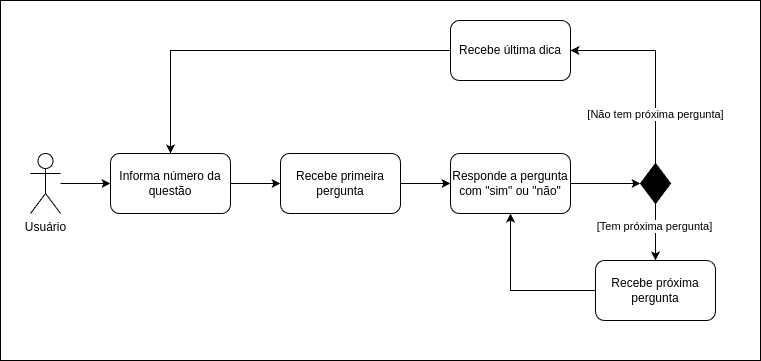
\includegraphics[scale=0.6]{pictures/atividade1.png}
        \fonte{Produzido pela autora.}
\end{figure}

A Figura 28 representa a estrutura da aplicação, mostrando a interação entre o frontend e o backend através de requisições. No frontend, o arquivo \textit{ActionProvider.tsx} gerencia as mensagens enviadas pelo usuário no chat, processando tanto o número da questão informada, quanto as respostas de "sim" ou "não". Por meio dessas requisições, o \textit{frontend} envia esses dados ao \textit{backend}, que, em resposta, fornece perguntas e dicas relacionadas à questão solicitada. Caso o usuário peça uma nova dica e o \textit{backend} não tenha mais sugestões para aquela questão, ele envia a orientação final da questão, que é então apresentada ao usuário.

\begin{figure}[h!]
    \centering
            \caption{Arquitetura da Aplicação do Sistema Especialista}
            \label{fig:ModeloConceitual}
        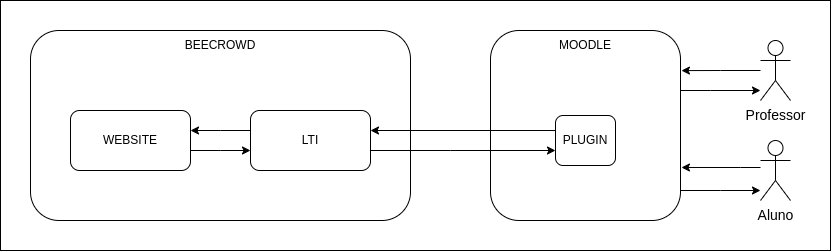
\includegraphics[scale=0.6]{pictures/arquitetura.png}
        \fonte{Produzido pela autora.}
\end{figure}


\subsection{Comunicação Frontend-Backend}

O Código 1 representa como o arquivo \textit{ActionProvider.tsx} informa para o backend o número da questão. Ele define duas funções assíncronas: \texttt{fetchData} e \texttt{handleFirstMessage}, usadas para interagir com um \textit{backend} via requisições HTTP. A função \texttt{fetchData} recebe uma URL e um corpo de dados (\texttt{URLSearchParams}) para fazer uma requisição \texttt{POST}. Ela define cabeçalhos para enviar os dados como \texttt{application/x-www-form-urlencoded}, garantindo que o backend receba os dados em um formato compatível e de fácil manipulação, especialmente em linguagens que interpretam parâmetros de URL de forma nativa. Além disso, a função inclui cookies nas requisições com \texttt{credentials: 'include'} para permitir que a sessão seja mantida entre as requisições, o que é crucial para a continuidade da comunicação com o backend. Caso a resposta não tenha o status 200, a função trata o erro, retornando uma mensagem de erro em vez do JSON da resposta. 

A função \texttt{handleFirstMessage} constrói um corpo de dados contendo \texttt{questionNumber} e chama \texttt{fetchData} para enviar esses dados ao \textit{backend} no endpoint \texttt{"http://localhost:6358/server"}. Em seguida, cria uma estrutura de mensagens adicionais vazia e invoca \texttt{handleMessageResponse} para manipular a resposta, preenchendo essa estrutura conforme a resposta recebida.

\begin{lstlisting}[style=ufscthesisx_style, caption={Funções assíncronas para requisição HTTP}]
    const fetchData = async (url: string, body: URLSearchParams) => {
        try {
            const response = await fetch(url, {
            method: "POST",
            headers: { 'Content-Type': 'application/x-www-form-urlencoded;charset=UTF-8' },
            credentials: 'include',
            body,
            });
    
            if (response.status !== 200) throw new Error("Erro ao consultar o backend.");
    
            return await response.json();
        } catch (error) {
            return { error: "Erro ao consultar o backend." };
        }
    };

const handleFirstMessage = async (questionNumber?: string) => {
    const body = new URLSearchParams({ questionNumber: questionNumber?.toString() || '' });
    const data = await fetchData("http://localhost:6358/server", body);
    let additionalMessages: {
        messages: {
        message: string;
        type: string;
        id: number;
        loading?: boolean;
        widget?: string | undefined;
        delay?: number | undefined;
        payload?: any;
        }[];
    }[] = [];

    await handleMessageResponse(data, additionalMessages);
};
\end{lstlisting}

\subsection{Elementos do Backend}

Pela Figura 28 também observa-se que o \textit{backend} é composto pelo arquivo principal \textit{server.pl} e por arquivos específicos para cada questão, nomeados no formato \textit{questao\_\{numeroDaQuestao\}.pl}, onde cada um contém dicas voltadas para uma questão particular. Por exemplo, o arquivo \textit{questao\_1234.pl} armazena as orientações para a questão 1234 do Beecrowd.

\subsubsection{Arquivos no formato questao\_\{numeroDaQuestao\}.pl}

O Código 2 apresenta o arquivo \textit{questao\_1181.pl} como um exemplo de estrutura para arquivos do tipo \textit{questao\_\{numeroDaQuestao\}.pl}.

\begin{lstlisting}[style=ufscthesisx_style, caption={Arquivo \textit{questao\_1181.pl}}]
    :- module(questao_1181, [questao/3, diagnostico/3]).
    
    % Predicado para fornecer perguntas com base na sequência de respostas
    questao(1181, [], "Você já desenvolveu sua solução, mas não está saíndo a resposta correta?").
    questao(1181, ["sim"], "Tome cuidado que a questão quer todos os elementos da linha, e não da coluna! Verifique \ccomo você está iterando sobre a matriz: se está pegando todos os elementos de uma linha \c ou todos os elementos de uma coluna. Mais uma dica sobre isso?").
    questao(1181, ["sim", "sim"], "Se sua matriz é feita de forma que é iterada assim: matriz[linha][coluna], verifique \cse o 'for' está correto. Quer saber como o for fica?").
    questao(1181, ["sim", "sim", "sim"], "considerando que l é a entrada do usuário que indica a linha que será a \cconsiderada para operação: \nfor i in range(0, 12): soma += matriz[l][i]. \n\cPróxima dica?").
    questao(1181, ["sim", "sim", "sim", "sim"], "Verifique se o número pelo qual você está tentando dividir para \cpara conseguir a média está correto. Próxima pergunta?").
    
    
    questao(1181, Respostas, "Deu Presentation Error?") :-
        Respostas = ["não"];
        Respostas = ["sim", "não"];
        Respostas = ["sim", "sim", "não"];
        Respostas = ["sim", "sim", "sim", "não"];
        Respostas = ["sim", "sim", "sim", "sim", "sim"].
    
    questao(1181, Respostas, "Perceba que a formatação que a questão pede é: Imprima o resultado solicitado \c(a soma ou média), com 1 casa após o ponto decimal. Ou seja, '%.1f'. Deu certo?") :-
        Respostas = ["não", "sim"];
        Respostas = ["sim", "não", "sim"];
        Respostas = ["sim", "sim", "não", "sim"];
        Respostas = ["sim", "sim", "sim", "não", "sim"];
        Respostas = ["sim", "sim", "sim", "sim", "sim", "sim"].
    
    
    % Diagnóstico com base nas respostas completas
    diagnostico(1181, Respostas, "Legal! Parabéns!") :-
        Respostas = ["não", "sim", "sim"];
        Respostas = ["sim", "não", "sim", "sim"];
        Respostas = ["sim", "sim", "não", "sim", "sim"];
        Respostas = ["sim", "sim", "sim", "não", "sim", "sim"];
        Respostas = ["sim", "sim", "sim", "sim", "não", "sim", "sim"].
    
    diagnostico(1181, _, "Atente-se bem às dicas já enviadas ou pergunte novamente! Além disso, você pode \cusar o udebug para verificar a diferença entre as saídas do seu código, e as \csaídas esperadas pela questão! Também é uma boa ideia debugar seu código no Thonny, \crevisando linha por linha, ou usando prints para entender o que ele está executando!").
\end{lstlisting}    

Esse arquivo Prolog define um módulo especializado para auxiliar usuários na resolução da questão 1181 por meio de um sistema especialista baseado em regras. O módulo \textit{questao\_1181} implementa dois predicados principais: \textit{questao/3} e \textit{diagnostico/3}, que são responsáveis por operacionalizar a lógica de suporte do sistema.

\begin{itemize}
    \item \textbf{Predicado \textit{questao/3}:} Este predicado orienta o usuário de maneira sequencial, adaptando as instruções com base nas respostas fornecidas. Ele recebe três parâmetros: o identificador da questão, uma lista de respostas (que mantém o histórico de interações), e uma mensagem de orientação. A matriz de decisões, implementada neste predicado, direciona o fluxo de perguntas e respostas com base no histórico de interações do usuário, promovendo uma progressão lógica que facilita a resolução da questão. Essa matriz está estruturada de forma que cada combinação de respostas leva a uma nova instrução, que oferece dicas cada vez mais específicas até que o usuário obtenha a solução correta.

    A tabela 2 apresenta a matriz de decisões para o predicado \textit{questao/3}, em formato de tabela, representando as combinações de respostas possíveis e as respectivas instruções emitidas:

    \begin{longtable}{|c|p{5cm}|p{8cm}|}
        \caption{Matriz de Decisões para o Predicado \textit{questao/3} na Questão 1181} \\
        \hline
        \textbf{Questão} & \textbf{Respostas} & \textbf{Instrução} \\
        \hline
        \endfirsthead
        \multicolumn{3}{|c|}{\textbf{Continuação da Tabela}} \\
        \hline
        \textbf{Questão} & \textbf{Respostas} & \textbf{Instrução} \\
        \hline
        \endhead
        \hline
        \endfoot
        \hline
        \endlastfoot
        
        1181 & [] & Você já desenvolveu sua solução, mas não está saindo a resposta correta? \\
        \hline
        1181 & [sim] & Tome cuidado que a questão quer todos os elementos da linha, e não da coluna! Verifique como você está iterando sobre a matriz: se está pegando todos os elementos de uma linha ou todos os elementos de uma coluna. Mais uma dica sobre isso? \\
        \hline
        1181 & [sim, sim] & Se sua matriz é feita de forma que é iterada assim: matriz[linha][coluna], verifique se o 'for' está correto. Quer saber como o for fica? \\
        \hline
        1181 & [sim, sim, sim] & Considerando que l é a entrada do usuário que indica a linha que será considerada para operação: \texttt{for i in range(0, 12): soma += matriz[l][i]} \newline Próxima dica? \\
        \hline
        1181 & [sim, sim, sim, sim] & Verifique se o número pelo qual você está tentando dividir para calcular a média está correto. Próxima pergunta? \\
        \hline
        1181 & [não], [sim, não], [sim, sim, não], [sim, sim, sim, não], [sim, sim, sim, sim, sim] & Deu Presentation Error? \\
        \hline
        1181 & [não, sim], [sim, não, sim], [sim, sim, não, sim], [sim, sim, sim, não, sim], [sim, sim, sim, sim, sim, sim] & Perceba que a formatação que a questão pede é: Imprima o resultado solicitado (a soma ou média), com 1 casa após o ponto decimal. Ou seja, \%.1f. Deu certo? \\
      \end{longtable}
    
    \item \textbf{Predicado \textit{diagnostico/3}:} Este predicado fornece um diagnóstico final com base nas respostas acumuladas ao longo da interação. Atuando como feedback conclusivo, ele emite uma mensagem de sucesso caso as respostas indiquem que o usuário compreendeu e solucionou a questão. Caso contrário, sugere ferramentas como o \textit{udebug} e o depurador \textit{Thonny}, de modo que o usuário possa inspecionar o comportamento do seu código em detalhes.
\end{itemize}

Dessa forma, arquivos do formato \textit{questao\_\{numeroDaQuestao\}.pl} devem seguir essa estrutura, onde cada questão contém um predicado \textit{questao/3} para fornecer orientações sequenciais e um predicado \textit{diagnostico/3} para avaliação final. A matriz de decisões implementada no predicado \textit{questao/3} permite um processo dinâmico e adaptativo de interação, guiando o usuário de forma direcionada e progressiva na resolução da questão específica.

\subsubsection{Arquivo server.pl}

\subsubsubsection{Configurando servidor HTTP}

O arquivo \textit{server.pl} configura e inicializa um servidor HTTP, definindo rotas para processar requisições e habilitando o CORS, permitindo conexões da porta do \textit{frontend}. Ele recebe requisições \textit{POST} para iniciar ou continuar uma questão, associando cada sessão ao usuário correspondente, e também aceita requisições \textit{GET} para fornecer o diagnóstico final com base nas respostas acumuladas durante a interação.

O Código 3 exemplifica a configuração de um servidor HTTP em Prolog utilizando o módulo \texttt{http\_dispatch}, no qual as rotas são definidas por meio de \texttt{http\_handler} para manipular requisições \textit{GET}, \textit{POST} e \textit{OPTIONS}. Especificamente, a requisição \textit{POST} é tratada pela rota \texttt{server}, sendo manipulada pela função \texttt{handle\_post\_request}.

\begin{lstlisting}[style=ufscthesisx_style, caption={Arquivo \textit{server.pl} - \textit{Handlers} e Manipuladores de requisições}]
% Define o handler para receber as requisições HTTP POST
:- http_handler(root(server), handle_post_request, [method(post)]).
:- http_handler(root(.), handle_options, [method(options)]).

% Manipulador de requisições POST
handle_post_request(Request) :-
    member(method(post), Request), !,
    
    % Garante que a sessão está ativa para o cliente
    http_session_id(_SessionID),

    % Lê os dados da requisição
    http_read_data(Request, Data, [encoding(utf8)]),

    % Definindo os headers para permitir CORS
    format('Access-Control-Allow-Origin: http://localhost:5173~n'),
    format('Access-Control-Allow-Credentials: true~n'),
    format('Content-Type: application/json; charset=UTF-8'),
    cors_enable(Request, [methods([post])]),

    (   % Caso seja a primeira requisição da questão
        member(questionNumber=QN, Data) 
    ->  % Inicializa a sessão e a questão
        http_session_retractall(questionNumber(_)),
        http_session_retractall(answers("Answers", _)),
        http_session_assert(answers("Answers", [])),
        
        http_session_assert(questionNumber(QN)),
        start_question(QN, FirstQuestion),

        reply_json_dict(FirstQuestion)

    ;   % Caso receba respostas subsequentes
        member(answer=Answer, Data),
        
        % Garante que a sessão tenha a variável questionNumber
        ( http_session_data(questionNumber(QN)) ->
            continue_question(QN, Answer, NextQuestionOrResult),
            reply_json_dict(NextQuestionOrResult)
        ;   % Erro caso a sessão não tenha um questionNumber
            reply_json_dict(_{error: "Número da questão não encontrado na sessão"})
        )
    ).
\end{lstlisting}    

O \textbf{manipulador de requisições POST} (\texttt{handle\_post\_request}) tem como função processar requisições \textit{POST} enviadas ao servidor, gerenciando o fluxo de perguntas e respostas entre o cliente e o servidor. Inicialmente, ele habilita o CORS, permitindo requisições provenientes do frontend no endereço \texttt{http://localhost:5173}, além de configurar os cabeçalhos necessários para o envio de credenciais, como cookies de sessão. A função verifica se a sessão está ativa, garantindo a associação com um ID de sessão único.

Dependendo do tipo de requisição, a função processa a primeira pergunta ou continua a sequência de perguntas baseadas nas respostas anteriores. Se for a primeira requisição, o número da questão é extraído, e a sessão é inicializada com os dados necessários. Além disso, o arquivo correspondente à questão é carregado dinamicamente. 

Caso seja uma resposta subsequente, a função valida a presença do número da questão na sessão, atualiza as respostas e retorna a próxima pergunta ou o resultado final. Se os dados da sessão estiverem faltando, um erro é enviado indicando que o número da questão não foi encontrado.

\subsubsubsection{Carregando os arquivos das questões}

Os arquivos de questões são carregados dinamicamente no \textit{server.pl} com base no número da questão recebido nas requisições \textit{POST}. Se o usuário alterna para uma nova questão, por exemplo, a questão Y, o \textit{backend} carrega o arquivo \textit{questao\_Y.pl} e passa a conduzir a interação de acordo com suas informações. 

No Código 4, é mostrado o trecho do \texttt{server.pl} que realiza esse carregamento dinâmico. O predicado \texttt{start\_question/2} tem como objetivo inicializar uma nova questão dentro de um sistema interativo, baseado no número da questão fornecido. O primeiro passo do código é construir o caminho para o arquivo que contém a definição da questão, concatenando o prefixo \texttt{questao\_} com o número da questão \texttt{(QuestionNumber)} e adicionando a extensão \texttt{.pl} para formar o nome completo do arquivo. Isso é realizado através do predicado \texttt{atom\_concat\/3}, que concatena átomos (strings) para formar o caminho completo do arquivo a ser carregado.

\begin{lstlisting}[style=ufscthesisx_style, caption={Arquivo \textit{server.pl} - \textit{Handlers} e Manipuladores de requisições}]
start_question(QuestionNumber, FirstQuestion) :-
    atom_concat('questao_', QuestionNumber, FileName),
    atom_concat(FileName, '.pl', FilePath),

    % Verifica se o arquivo existe antes de tentar carregá-lo
    (   exists_file(FilePath)
    ->  % Carrega dinamicamente o arquivo da questão
        abolish(questao/3),
        abolish(diagnostico/3),

        ensure_loaded(FilePath)
    ).
\end{lstlisting}

Depois, o código verifica se o arquivo gerado existe no sistema de arquivos utilizando o predicado \texttt{exists\_file\/1}. Caso o arquivo exista, o sistema prossegue para carregá-lo dinamicamente com o predicado \texttt{ensure\_loaded\/1}. Antes de carregar o arquivo, o predicado \texttt{abolish\/1} é utilizado para garantir que qualquer definição anterior dos predicados \texttt{questao\/3} e \texttt{diagnostico\/3} seja removida da memória, evitando conflitos ou sobrecarga de definições antigas.

\subsubsubsection{Recebe respostas}

O arquivo \textit{server.pl} também armazena na sessão do usuário as informações fornecidas, como número da questão e respostas, para garantir a continuidade da interação. O Código 5 apresenta a função \textbf{continue\_question}, responsável por processar respostas subsequentes enviadas pelo usuário para uma questão em andamento, armazenando a resposta na sessão e determinando o próximo passo com base nas respostas acumuladas. Inicialmente, a função adiciona a nova resposta à lista de respostas da sessão, atualizando a variável de sessão \texttt{answers("Answers")}. Em seguida, tenta gerar a próxima pergunta por meio da chamada ao predicado \texttt{questao/3}. Se \texttt{questao/3} retornar uma nova pergunta (\texttt{NextQuestion}), esta é enviada ao cliente para dar continuidade à interação. Caso contrário, a função verifica se uma resposta final pode ser gerada utilizando o predicado \texttt{diagnostico/3}. O resultado final, seja uma nova pergunta ou uma conclusão, é então enviado ao cliente no formato JSON, permitindo que a interação prossiga ou seja concluída de acordo com o progresso da sessão.

\begin{lstlisting}[style=ufscthesisx_style, caption={Arquivo \textit{server.pl} - \textit{Handlers} e Manipuladores de requisições}]
continue_question(QuestionNumber, Answer, Response) :-
    (   string(Answer) -> AW = Answer
    ;   atom(Answer) -> atom_string(Answer, AW)
    ;   term_string(Answer, AW)
    ),
    atom_number(QuestionNumber, QN), 

    % Salva a resposta na sessão
    http_session_data(answers("Answers", AnswerList)),
    append(AnswerList, [AW], UpdatedAnswers),
    http_session_retractall(answers("Answers", _)),
    http_session_assert(answers("Answers", UpdatedAnswers)),

    % Chama a questão correspondente com a lista atualizada de respostas
    (   questao(QN, UpdatedAnswers, NextQuestion)
    ->  Response = _{question: NextQuestion}
    ;   (   diagnostico(QN, UpdatedAnswers, Result)
        ->  true
        ;   Result = "Sem conclusão final."
        ),
        Response = _{result: Result}
    ).

\end{lstlisting}

\subsection{Elementos do Frontend}

\end{otherlanguage*}



    % PARTE
    %\ifforcedinclude\else\part{\lang{Implementation}{Implementação}}\fi
    %\label{segunda_parte}

    % Segundo capitulo de Resultados
    
% The \phantomsection command is needed to create a link to a place in the document that is not a
% figure, equation, table, section, subsection, chapter, etc.
% https://tex.stackexchange.com/questions/44088/when-do-i-need-to-invoke-phantomsection
\phantomsection

% Multiple-language document - babel - selectlanguage vs begin/end{otherlanguage}
% https://tex.stackexchange.com/questions/36526/multiple-language-document-babel-selectlanguage-vs-begin-endotherlanguage
\begin{otherlanguage*}{brazil}

\chapter{Validação}

Nesta seção, será realizada uma análise crítica da proposta, abordando as vantagens e desvantagens da integração entre o Moodle e o Beecrowd via LTI (\textit{Learning Tools Interoperability}), bem como da aplicação da aplicação com sistema especialista desenvolvida. Além disso, será apresentada uma avaliação prática sobre o uso da aplicação pelos alunos da disciplina \textit{Programação Orientada a Objetos I} da Universidade Federal de Santa Catarina (UFSC) no segundo semestre de 2024, com o objetivo de verificar se o sistema especialista conseguiu resolver efetivamente as dúvidas dos estudantes.

\section{Integração LTI entre o Moodle e o Beecrowd}

\subsection{Vantagens}
\begin{itemize}
    \item \textbf{Vantagens do Beecrowd:} O Beecrowd oferece uma plataforma robusta para a resolução de problemas de programação, com uma grande variedade de questões que permitem aos alunos praticar e desenvolver habilidades de programação em diversos níveis de dificuldade. A plataforma também facilita o acompanhamento do progresso dos alunos, oferecendo métricas e \textit{feedback} instantâneo sobre o desempenho nas questões.
    \item \textbf{Facilidade de acesso através da integração LTI:} A integração LTI simplifica o acesso ao Beecrowd, pois tanto o professor quanto o aluno podem acessar a plataforma diretamente do Moodle com um único clique.
\end{itemize}

\subsection{Desvantagens}
\begin{itemize}
    \item \textbf{Desenvolvimento externo e curva de aprendizado:} O desenvolvimento dos códigos e a criação das listas de exercícios ainda ocorre fora do Moodle, no Beecrowd, o que significa que o professor precisa aprender a usar o Beecrowd Academic, embora o processo seja relativamente simples. Isso pode exigir um tempo adicional de adaptação, especialmente para aqueles que não estão familiarizados com a plataforma.
\end{itemize}

\section{Sistema Especialista para Resolução de Dúvidas no Beecrowd}

\subsection{Vantagens}
\begin{itemize}
    \item \textbf{Atendimento automatizado:} O sistema especialista pode fornecer respostas rápidas e precisas para questões frequentes ou comuns, permitindo que os alunos resolvam suas dúvidas sem a necessidade de intervenção humana constante.
    \item \textbf{Apoio no aprendizado:} O sistema pode ser configurado para fornecer explicações detalhadas sobre questões específicas do Beecrowd, ajudando os alunos a entender melhor os problemas e as soluções.
    \item \textbf{Escalabilidade:} Como o sistema é automatizado, ele pode lidar com um grande volume de dúvidas de maneira eficiente.
    \item \textbf{Redução da sobrecarga para os professores:} Ao automatizar o atendimento às dúvidas mais comuns, o sistema especialista permite que os professores se concentrem em questões mais complexas e em atividades pedagógicas, sem se sobrecarregar com um grande volume de perguntas repetitivas.
    \item \textbf{Auxílio para professores não familiarizados com o Beecrowd:} Para professores que ainda não estão familiarizados com as questões do Beecrowd, o sistema especialista oferece uma ferramenta valiosa para auxiliá-los a responder dúvidas dos alunos de maneira eficiente, sem a necessidade de um profundo conhecimento prévio sobre a plataforma ou as questões.
\end{itemize}

\subsection{Desvantagens}
\begin{itemize}
	\item \textbf{Limitação nas respostas para questões complexas:} O sistema especialista é eficiente para lidar com questões simples ou frequentes, mas pode encontrar dificuldades ao lidar com questões mais complexas ou específicas. Para adicionar suporte a novas questões, o professor precisa criar uma matriz de decisões detalhada, o que pode tornar o processo demorado e propenso a erros, especialmente quando se trata de questões que exigem uma análise mais aprofundada. Sem a devida cautela, o sistema pode acabar gerando respostas imprecisas ou inadequadas, comprometendo a qualidade das interações e a efetividade do suporte oferecido.
    \item \textbf{Dependência da qualidade da base de conhecimento:} O desempenho do sistema especialista depende diretamente da qualidade das regras e conhecimentos que foram programados nele. Se a base de dados for limitada ou desatualizada, o sistema pode fornecer respostas inadequadas.
    \item \textbf{Falta de interação humana:} Em casos onde o aluno necessita de uma explicação mais personalizada ou de orientação emocional, o sistema especialista pode não ser suficiente, criando uma experiência impessoal que pode não atender completamente às necessidades do aluno.
\end{itemize}

\section{Avaliação Prática}

A avaliação prática foi conduzida por meio da utilização do sistema especialista pelos alunos da disciplina \textit{Programação Orientada a Objetos I} da UFSC, durante o segundo semestre de 2024. Para isso, foram realizados os seguintes passos:

\begin{enumerate}
    \item \textbf{Aplicação do sistema:} Os alunos foram incentivados a usar o sistema especialista para resolver dúvidas relacionadas às questões do Beecrowd. Durante esse período, o uso do sistema foi monitorado para avaliar sua eficácia em termos de resolução de dúvidas.
    \item \textbf{Análise de resultados:} Foram avaliados o número de dúvidas resolvidas, as dúvidas não esclarecidas e os \textit{feedbacks} fornecidos pelos alunos.
    \item \textbf{Melhorias das questões:} Com base na análise dos resultados, dúvidas não resolvidas pelo Bee Expert foram incluídas no sistema para futuras turmas.
\end{enumerate}

É importante destacar que, até o momento, o Expert Bee tinha apenas dicas de resoluções para essas questões da lista de exercícios fornecida, e não dicas para dúvidas reais coletadas de alunos. Essas dicas de resoluções tinham sido disponibilizadas pelo professor durante a primeira coleta de dados, descrita na seção \ref{sec:coleta-dados}, para que fosse possível testar a eficácia da ferramenta na hora em que as dúvidas dos alunos surgiriam. 

Assim, um dos objetivos da avaliação prática também era identificar dúvidas não tratadas pelo Expert Bee, para que elas pudessem ser adicionadas à ferramenta.

\subsection{Resultados}  

Na Avaliação Prática realizada em 18 de novembro de 2024, foi disponibilizada aos alunos uma lista com as seguintes questões do Beecrowd: 1261, 1281, 1430, 1449, 1483, 1763, 1911, 1953, 2091, 2482, 2492, 2654, 2949 e 2987, para que começassem a resolver durante a aula. 12 alunos estiveram presente na sala de aula e, sempre que um aluno apresentava uma dúvida, ele utilizava primeiro o Expert Bee para tentar resolvê-la, e, caso não conseguisse, recorria ao professor. 

As dúvidas relatadas pelos alunos foram as seguintes:  

\begin{itemize}  
    \item \textbf{Questão 1911:} 4 alunos apresentaram dúvidas, e todos conseguiram resolvê-las apenas com o auxílio do Bee Expert.  
    \item \textbf{Questão 2654:} 2 alunos tiveram dúvidas, todas solucionadas pelo Bee Expert.  
    \item \textbf{Questão 1430:} 1 aluno apresentou dúvida e conseguiu resolvê-la com o Bee Expert.  
    \item \textbf{Questão 2949:} 1 aluno apresentou dúvida, solucionada pelo Bee Expert.  
    \item \textbf{Questão 1483:} 1 aluno teve dúvida, também solucionada pelo Bee Expert.  
    \item \textbf{Questão 1261:} 2 alunos apresentaram dúvidas específicas que não puderam ser resolvidas, pois o Bee Expert, à época, fornecia apenas uma ideia geral de resolução.  
\end{itemize}  

No total, de 11 dúvidas relatadas, o Bee Expert conseguiu resolver 9, resultando em uma taxa de sucesso de aproximadamente 81\%.  

\subsection{Pontos de Melhoria}  

\begin{itemize}  
    \item \textbf{Questão 1261:} As dúvidas específicas dos alunos foram incorporadas ao sistema, enriquecendo o conteúdo da questão para turmas futuras.  
    \item \textbf{Questões 1911 e 2654:} Apesar do sucesso na resolução, foi identificado um ponto de melhoria: o Bee Expert apresentava diretamente a solução completa após a primeira interação. No entanto, os alunos demonstraram interesse em orientações iniciais sobre como resolver as questões utilizando dicionários em Python. Esse ajuste foi implementado, permitindo ao usuário solicitar essas informações antes da solução.  
    \item \textbf{Questão 1430:} A dúvida do aluno surgiu por falta de entendimento do método \texttt{split()} do Python. Como melhoria, o arquivo dessa questão no Bee Expert agora inclui uma explicação detalhada sobre o uso do método.  
\end{itemize}  

\end{otherlanguage*}



    % Finaliza a parte no bookmark do PDF para que se inicie o bookmark na raiz
    % e adiciona espaço de parte no Sumário
    \phantompart

    % Conclusão (outro exemplo de capítulo sem numeração e presente no sumário)
    
% The \phantomsection command is needed to create a link to a place in the document that is not a
% figure, equation, table, section, subsection, chapter, etc.
% https://tex.stackexchange.com/questions/44088/when-do-i-need-to-invoke-phantomsection
\phantomsection

% ---
\chapter{\lang{Final Remarks}{Considerações Finais}}

Em conclusão, este trabalho abordou a relevância da integração de ferramentas tecnológicas no ensino de programação, com foco especial no uso de plataformas como Beecrowd e Moodle. A análise dos juízes online e outras plataformas educacionais, como o VPL, evidenciou desafios na usabilidade e na integração, mas também destacou o Beecrowd como uma solução eficaz para o ensino de algoritmos e programação, com recursos que incentivam o aprendizado ativo, como gamificação, feedback em tempo real e uma gama diversificada de questões.

Este estudo aprofundou o impacto dos juízes online no ensino de programação, enfatizando a relevância da integração entre plataformas como o Beecrowd e o Moodle. Foi realizada uma análise detalhada do Moodle, destacando suas funcionalidades e como ele pode ser integrado de forma eficiente ao Beecrowd para potencializar o processo de aprendizagem. A proposta de integração dessas duas plataformas, por meio de um plugin LTI (Learning Tools Interoperability) desenvolvido pelo Beecrowd, visa simplificar o ensino e tornar as atividades de programação mais acessíveis e eficazes para os alunos.

A integração do Beecrowd ao Moodle, por meio da tecnologia LTI, facilita o acesso de professores e alunos a uma vasta gama de questões, otimizando o uso da plataforma no ambiente acadêmico. Além disso, oferece uma interface amigável para a criação de listas de exercícios pelos professores e a resolução de problemas de programação pelos alunos. Com o objetivo de apoiar essa integração, foi desenvolvido um manual detalhado sobre como integrar o Moodle ao Beecrowd via LTI, bem como um guia para orientar os professores no uso da plataforma.

Para estimular o uso do Beecrowd no ambiente acadêmico, também foi criada uma ferramenta com um sistema especialista que auxilia os alunos ao esclarecer dúvidas recorrentes nas questões do Beecrowd. Esse sistema não só oferece suporte aos estudantes, mas também facilita a adaptação dos professores, promovendo um ambiente de aprendizado mais fluido e eficiente para todos os envolvidos.

\section{Trabalhos Futuros}

A seção a seguir apresenta algumas sugestões de melhorias e direções futuras para a aplicação de sistema especialista desenvolvida. 

\begin{itemize}
    \item  \textbf{Adição de dicas de novas questões pela interface web:} Uma melhoria importante seria permitir que os professores possam adicionar dicas para novas questões diretamente pela interface da aplicação web, sem a necessidade de modificar o código-fonte. Isso tornaria o sistema mais acessível e eficiente, permitindo que os educadores atualizem e personalizem o conteúdo de maneira prática e intuitiva, sem a dependência de habilidades técnicas.
    \item  \textbf{Sistema autoalimentado (aprendizado com as interações dos alunos):} Uma evolução significativa seria o desenvolvimento de um sistema que se autoalimente, aprendendo com as interações dos alunos. Esse sistema poderia analisar as dúvidas mais frequentes e adaptar-se automaticamente, oferecendo respostas e dicas mais precisas com o tempo. A implementação desse recurso resultaria em uma experiência de aprendizagem mais personalizada, ajudando os alunos a superarem suas dificuldades de maneira mais eficiente.
    \item  \textbf{Integração com ferramentas de processamento de linguagem natural (ChatGPT):} A integração do sistema especialista com ferramentas de processamento de linguagem natural, como o ChatGPT, permitiria uma interação mais fluida e natural entre os alunos e o sistema. Essa integração tornaria as respostas mais precisas, contextuais e dinâmicas, além de oferecer um nível maior de personalização nas interações, melhorando a qualidade do suporte oferecido.
\end{itemize}

\phantomsection




    % ELEMENTOS PÓS-TEXTUAIS
    \postextual
    \setlength\beforechapskip{0pt}
    \setlength\midchapskip{15pt}
    \setlength\afterchapskip{15pt}

    % Referências bibliográficas
    \begingroup
        % https://tex.stackexchange.com/questions/163559/how-to-modify-line-spacing-per-entry-of-bibliography
        % https://tex.stackexchange.com/questions/19105/how-can-i-put-more-space-between-bibliography-entries-biblatex
        \setlength\bibitemsep{\baselineskip}
        \advisor{}{\linespread{1.18}\selectfont}

        % https://tex.stackexchange.com/questions/17128/using-bibtex-to-make-a-list-of-references-without-having-citations-in-the-body
        % \nocite{*}
        \printbibliography[title=\lang{REFERENCES}{REFERÊNCIAS}]
    \endgroup

    % Glossário, consulte o manual da classe abntex2 para orientações sobre o glossário.
    % \ifforcedinclude\else\glossary\fi

    % Inicia os apêndices
    \begin{apendicesenv}
        % Imprime uma página indicando o início dos apêndices
        \ifforcedinclude\else\partapendices\fi
        \setlength\beforechapskip{50pt}
        \setlength\midchapskip{20pt}
        \setlength\afterchapskip{20pt}

        


%
% How to fix the Underfull \vbox badness has occurred while \output is active on my memoir chapter style?
% https://tex.stackexchange.com/questions/387881/how-to-fix-the-underfull-vbox-badness-has-occurred-while-output-is-active-on-m
%

% ---

\lang
% {\chapter[Page not filled]{Since this page is not being completely filled, it is generating the bottom bottom of the page}}
% {\chapter[Página não gerada]{Como esta página não está sendo completamente preenchida, ele está gerando a caixa inferior inferior da página}}
% ---


% Multiple-language document - babel - selectlanguage vs begin/end{otherlanguage}
% https://tex.stackexchange.com/questions/36526/multiple-language-document-babel-selectlanguage-vs-begin-endotherlanguage
\begin{otherlanguage*}{brazil}

\chapter{Manual de configuração da LTI Beecrowd no Moodle}
\label{manual:config-lti}

O administrador do Moodle deve configurar a LTI do Beecrowd.


\begin{enumerate}
    \item Acessar o moodle com uma conta de administrador
    \item Selecionar a opção: \textbf{Plugins}

    \begin{figure}[h!]
        \centering
            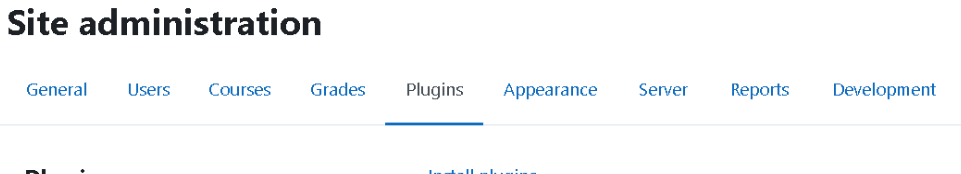
\includegraphics[scale=0.45]{pictures/apendices/apendice_a_1.png}
    \end{figure}

    \item Em Activity Modules, selecionar \textbf{External tool} -> \textbf{Manage tools}

    \begin{figure}[h!]
        \centering
            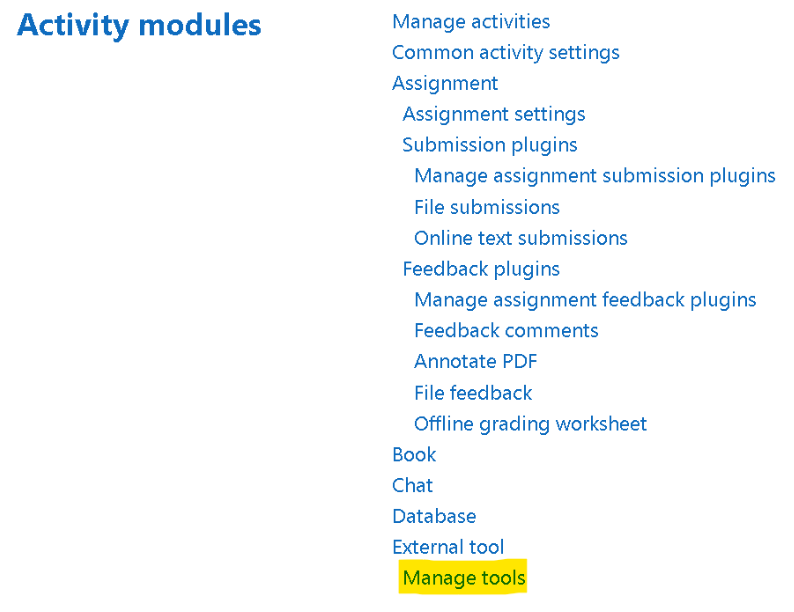
\includegraphics[scale=0.5]{pictures/apendices/apendice_a_2.png}
    \end{figure}

    \item Selecionar a opção \textbf{configure a tool manually}

    \begin{figure}[h!]
        \centering
            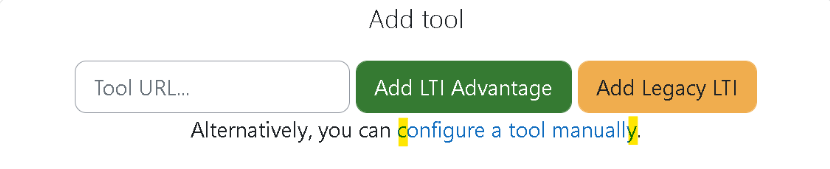
\includegraphics[scale=0.4]{pictures/apendices/apendice_a_3.png}
    \end{figure}

    \item Na página a seguir, preencher os campos conforme abaixo:\\

    Tool name: \textit{beecrowd} \\
    Tool URL: \textit{https://api.beecrowd.com/} \\
    Tool description: \textit{beecrowd LTI1.3 moodle integration} \\
    LTI version: \textit{LTI 1.3} \\
    Public key type: \textit{Keyset URL} \\
    Public keyset: \textit{https://api.beecrowd.com/lti/jwks} \\
    Initiate login URL: \textit{https://api.beecrowd.com/lti/login} \\
    Redirection URI(s): \textit{https://api.beecrowd.com/lti/launch} \\
    Custom parameters: “Manter vazio” \\
    Tool configuration usage: \textit{Show in activity chooser and as a preconfigured tool} \\
    Default launch container: \textit{New window} \\
    Supports Deep Linking (Content-Item Message): \textit{“Assinalar o check box”} \\
    Content Selection URL: \textit{https://api.beecrowd.com} \\
    
    Icon URL: \textit{https://moodle.beecrowd.io/pluginfile.php/15/course/summary/lgo.png} \\
    Secure icon URL: \textit{https://moodle.beecrowd.io/pluginfile.php/15/course/summary/lgo.png} \\
    
    \textbf{Services} \\
    IMS LTI Assignment and Grade Services:  \textit{Use this service for grade sync and column management} \\
    IMS LTI Names and Role Provisioning: \textit{Use this service to retrieve members' information as per privacy settings} \\
    Tool Settings: \textit{Use this service} \\
    
    \textbf{Privacy} \\
    Share launcher's name with tool: \textit{Always} \\
    Share launcher's email with tool: \textit{Always} \\
    Accept grades from the tool: \textit{Always} \\
    Force SSL: “Não assinalar” \\
    
    \textbf{Miscellaneous} \\
    Default organisation ID:  \textit{Site hostname} \\
    Organisation ID: “Manter Vazio” \\
    Organisation URL: \textit{https://beecrowd.com/} \\
    

    \item Após configurar as informações acima, você deve enviar para o Beecrowd a captura de tela da seguinte tela (exemplo na foto abaixo) através do botão de e-mail com os dados que eles devem inserir na parte deles para estabelecer a comunicação:
    
    \begin{figure}[h!]
        \centering
            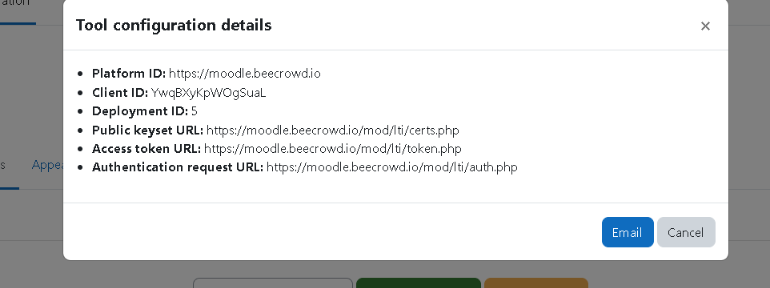
\includegraphics[scale=0.4]{pictures/apendices/apendice_a_5.png}
    \end{figure}
    
    \item Será exibida uma página de autorização. Basta preencher o email e aguardar a aprovação. Uma vez feito, é necessário recarregar a sessão e iniciar os testes novamente.

    \begin{figure}[h!]
        \centering
            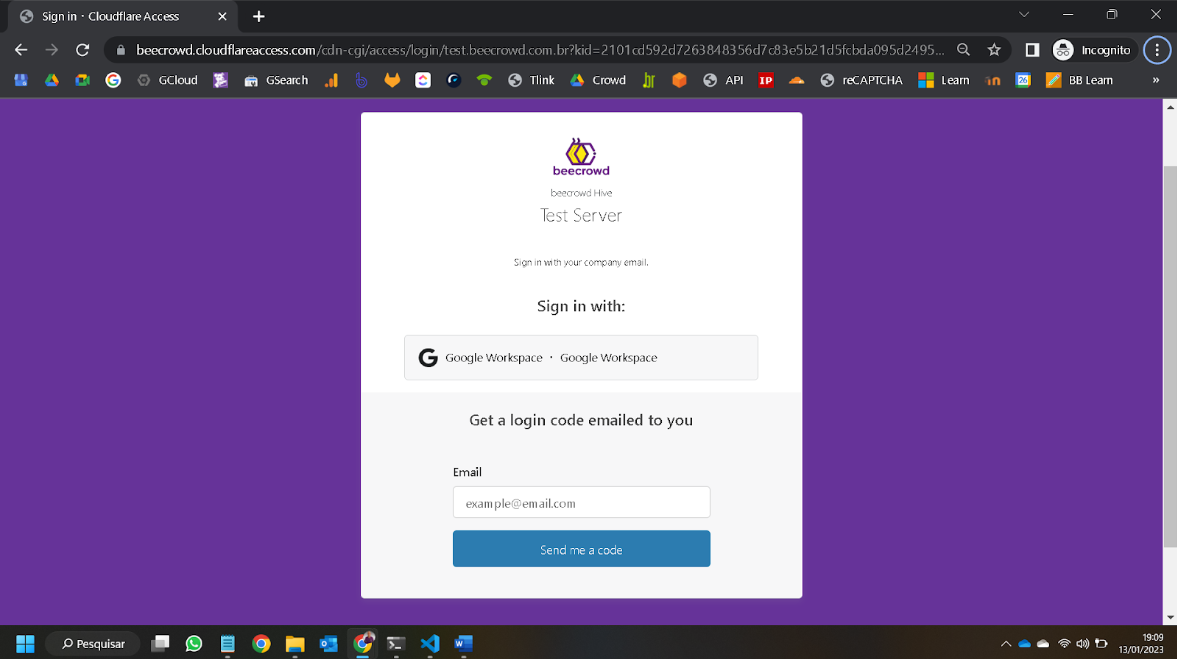
\includegraphics[scale=0.4]{pictures/apendices/apendice_a_6.png}
    \end{figure}

\end{enumerate}

\end{otherlanguage*}



        


%
% How to fix the Underfull \vbox badness has occurred while \output is active on my memoir chapter style?
% https://tex.stackexchange.com/questions/387881/how-to-fix-the-underfull-vbox-badness-has-occurred-while-output-is-active-on-m
%

% ---

\lang
% {\chapter[Page not filled]{Since this page is not being completely filled, it is generating the bottom bottom of the page}}
% {\chapter[Página não gerada]{Como esta página não está sendo completamente preenchida, ele está gerando a caixa inferior inferior da página}}
% ---


% Multiple-language document - babel - selectlanguage vs begin/end{otherlanguage}
% https://tex.stackexchange.com/questions/36526/multiple-language-document-babel-selectlanguage-vs-begin-endotherlanguage
\begin{otherlanguage*}{brazil}

\chapter{Manual de uso LTI Beecrowd no Moodle}

\subsection{Utilizar LTI do Beecrowd já configurada no Moodle}

Este Manual mostra como o professor cria uma atividade Beecrowd no Moodle, como um aluno acessa essa atividade, e como o professor pode transferir as notas do Beecrowd para o Moodle.

\subsection{Criando a atividade}

\begin{enumerate}
    \item Entre em modo edição
    \item Vá em adicionar uma atividade ou recurso:

    \begin{figure}[H]
        \centering
            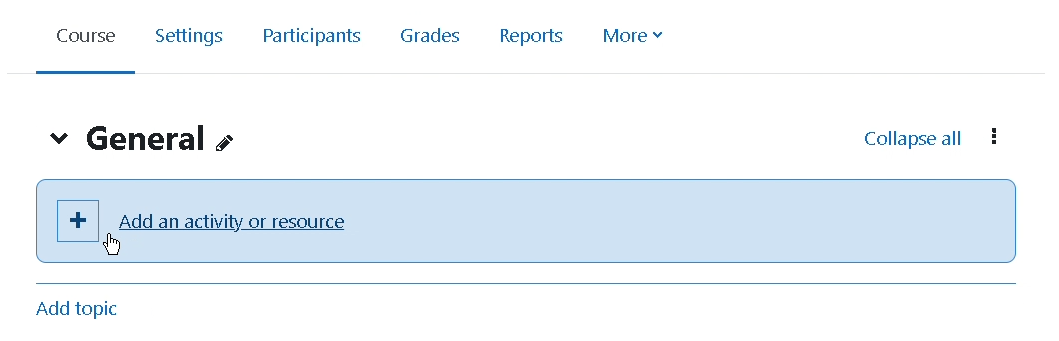
\includegraphics[scale=0.425]{pictures/apendices/apendice_b_1.png}
    \end{figure}

    \item Selecione a atividade “beecrowd”

    \begin{figure}[H]
        \centering
            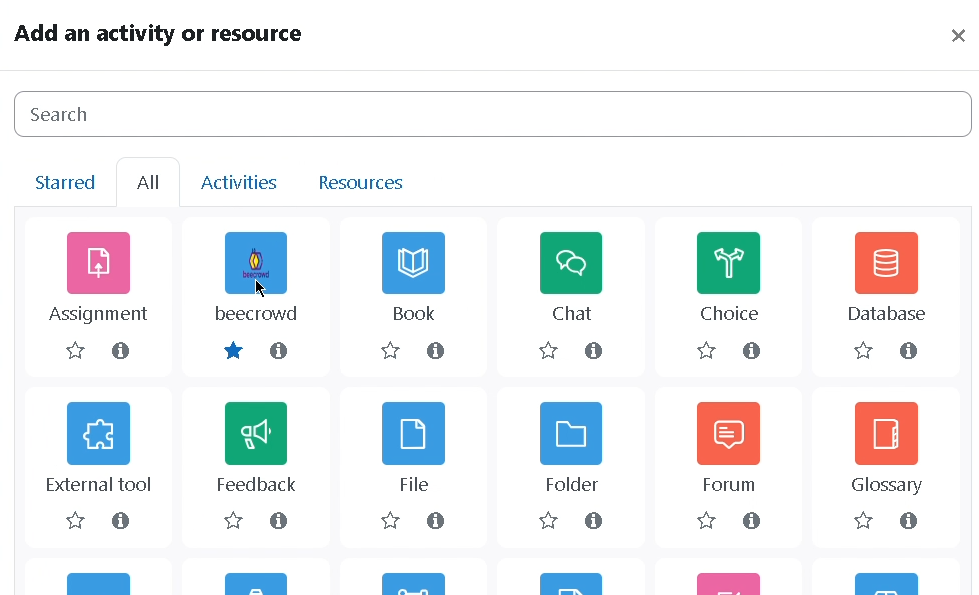
\includegraphics[scale=0.45]{pictures/apendices/apendice_b_2.png}
    \end{figure}

    \item Na página que abrir:

    \begin{enumerate}
        \item Em \textbf{General} > \textbf{Activity Name}, escreva o nome da atividade - como essa primeira vai ser para uso do professor, para entrar no Beecrowd Academic, você pode escolher um nome tipo \textit{“Acesso ao Beecrowd Acadêmico”};
        \item Em \textbf{Grade} > \textbf{Type}, selecione \textit{None};
        \item Em \textbf{Common module settings} > \textbf{Availability}, selecione \textit{“Hidden on Course Page”};
        \item Clique em \textbf{Save and return to course}.
    \end{enumerate}

    \begin{figure}[H]
        \centering
            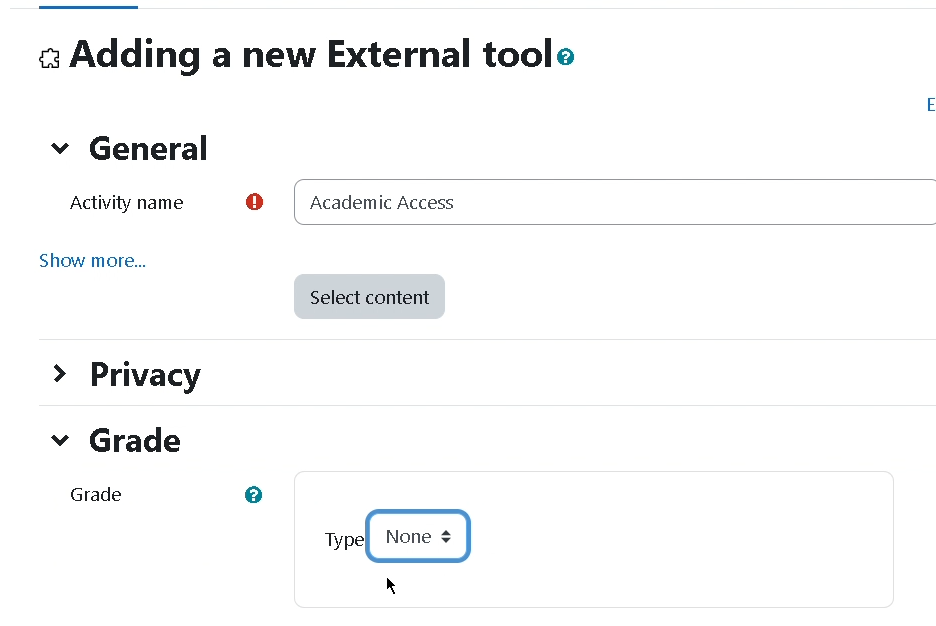
\includegraphics[scale=0.4]{pictures/apendices/apendice_b_3.png}
    \end{figure}

    \begin{figure}[H]
        \centering
            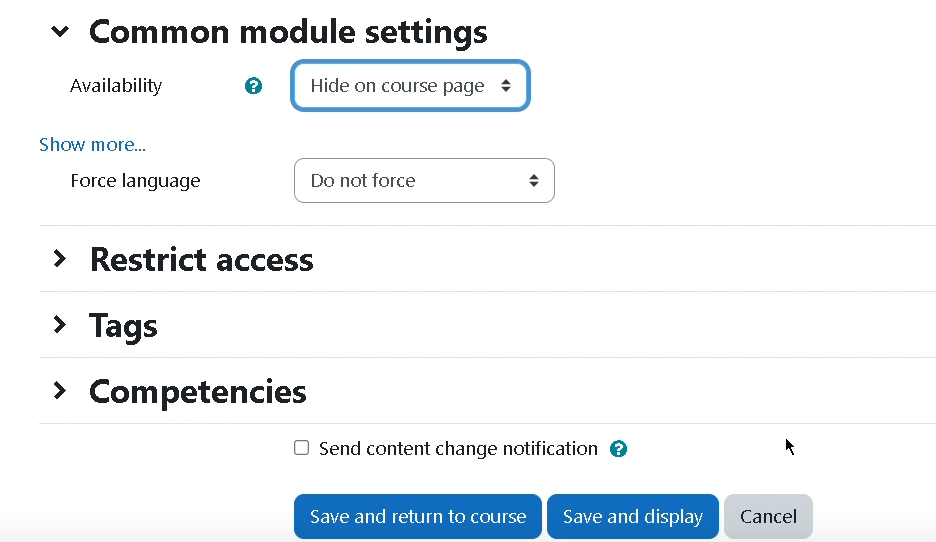
\includegraphics[scale=0.4]{pictures/apendices/apendice_b_4.png}
    \end{figure}

    \item Agora, a atividade que você criou vai aparecer na página do curso. Clique nela.

    \begin{figure}[H]
        \centering
            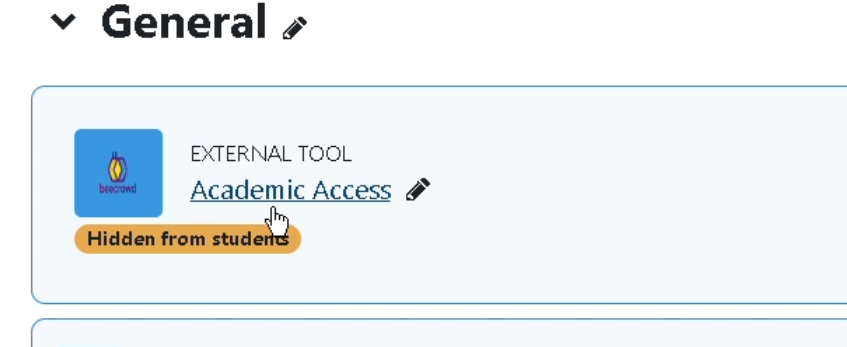
\includegraphics[scale=0.3]{pictures/apendices/apendice_b_5.png}
    \end{figure}

    \item Você vai ser redirecionado para a página do Beecrowd Academic. Caso você já esteja logado, vai aparecer a lista de suas disciplinas.    
    \begin{figure}[H]
        \centering
            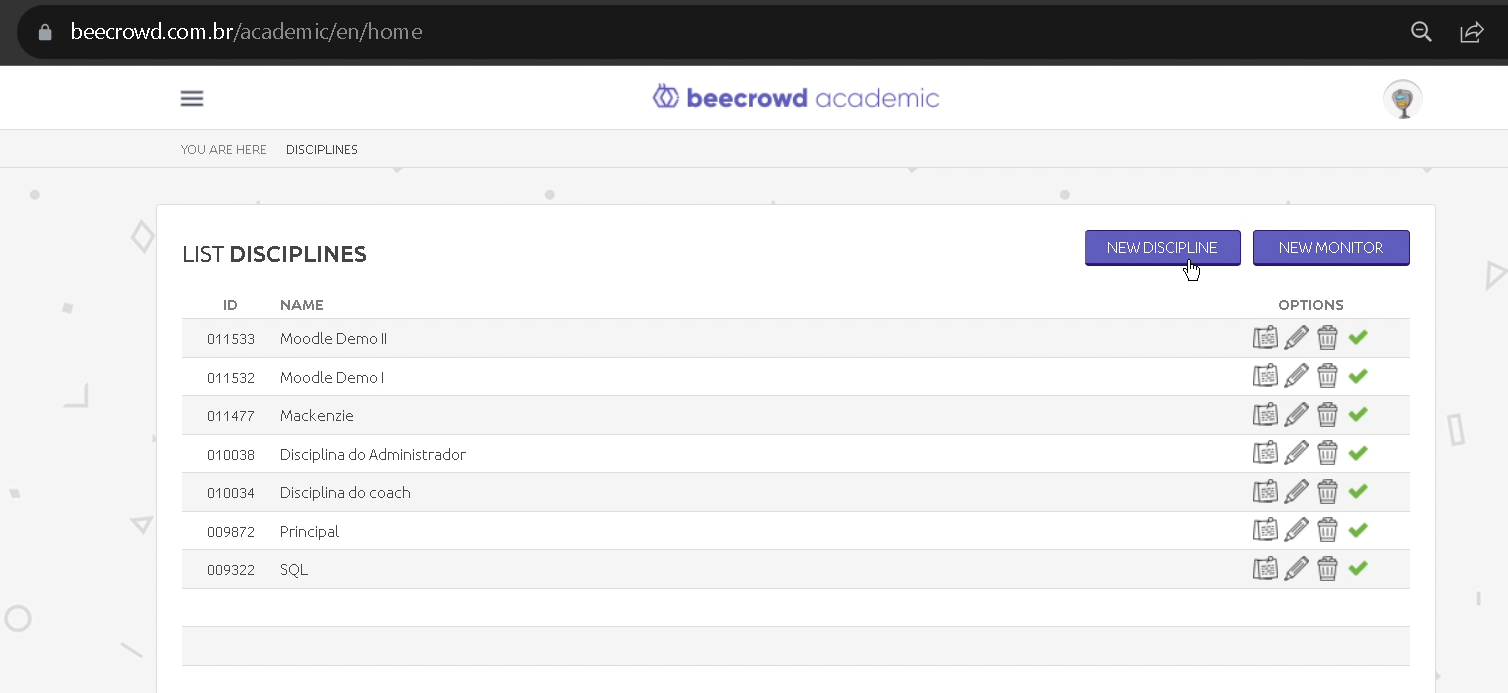
\includegraphics[scale=0.3]{pictures/apendices/apendice_b_6.png}
    \end{figure}

    Você pode criar uma disciplina, ou selecionar uma disciplina já existente. Para cada disciplina, você pode criar tarefas, e, para cada tarefa, você pode selecionar diferentes questões, e arrumar outras configurações, como data de início, de fim, etc (Veja as imagens da próxima página).

    Criar ou editar tarefa:

    \begin{figure}[H]
        \centering
            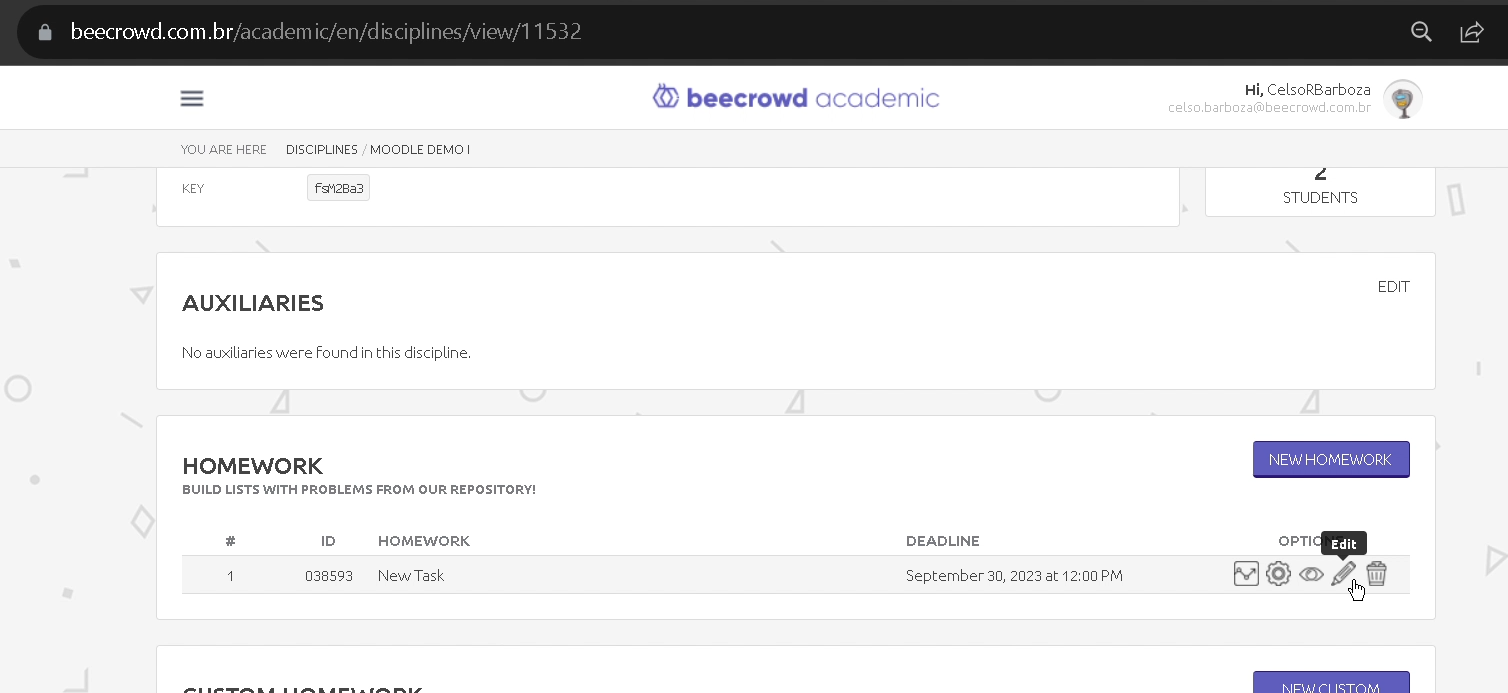
\includegraphics[scale=0.3]{pictures/apendices/apendice_b_7.png}
    \end{figure}

    Editando a tarefa:

    \begin{figure}[H]
        \centering
            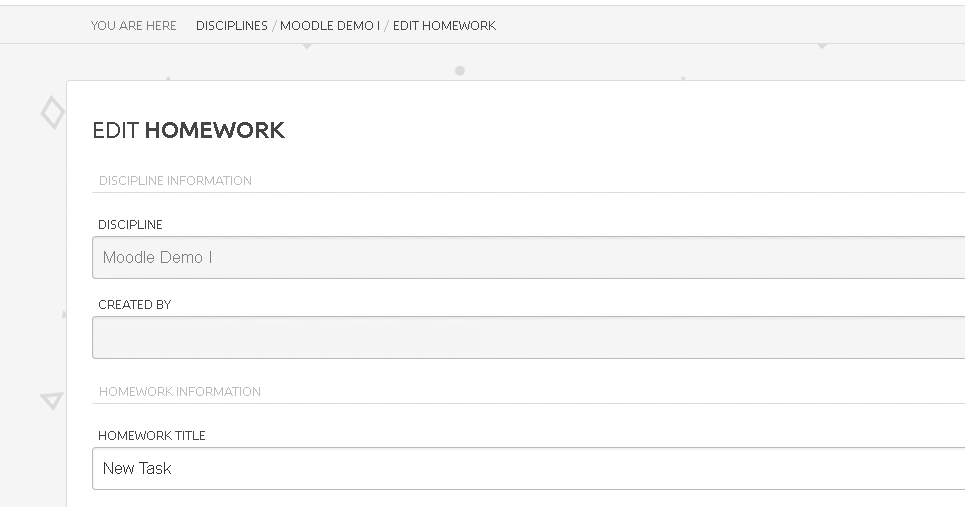
\includegraphics[scale=0.4]{pictures/apendices/apendice_b_8.png}
    \end{figure}

    Selecionando questões:

    \begin{figure}[H]
        \centering
            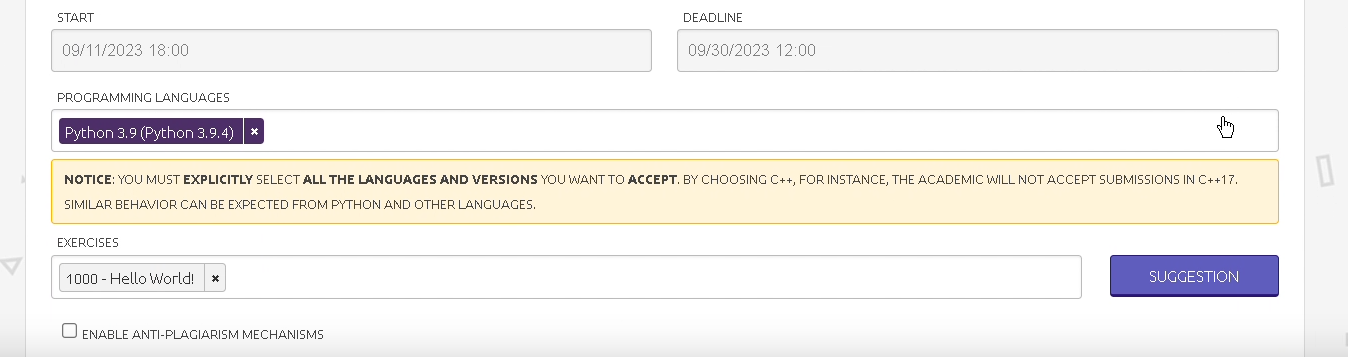
\includegraphics[scale=0.3]{pictures/apendices/apendice_b_9.png}
    \end{figure}
    
    \item Agora que você tem a disciplina com a tarefa desejada, volte ao Moodle e clique para adicionar uma atividade ou recurso:

    \begin{figure}[H]
        \centering
            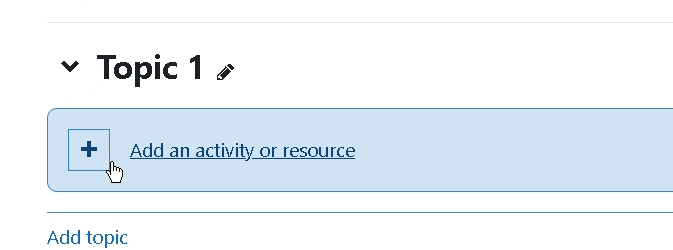
\includegraphics[scale=0.3]{pictures/apendices/apendice_b_10.png}
    \end{figure}

    \item Selecione a atividade Beecrowd:

    \begin{figure}[H]
        \centering
            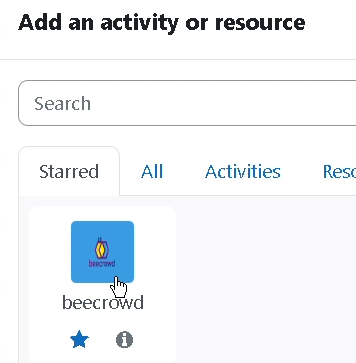
\includegraphics[scale=0.4]{pictures/apendices/apendice_b_11.png}
    \end{figure}

    \item Clique em “Selecionar conteúdo”:

    \begin{figure}[H]
        \centering
            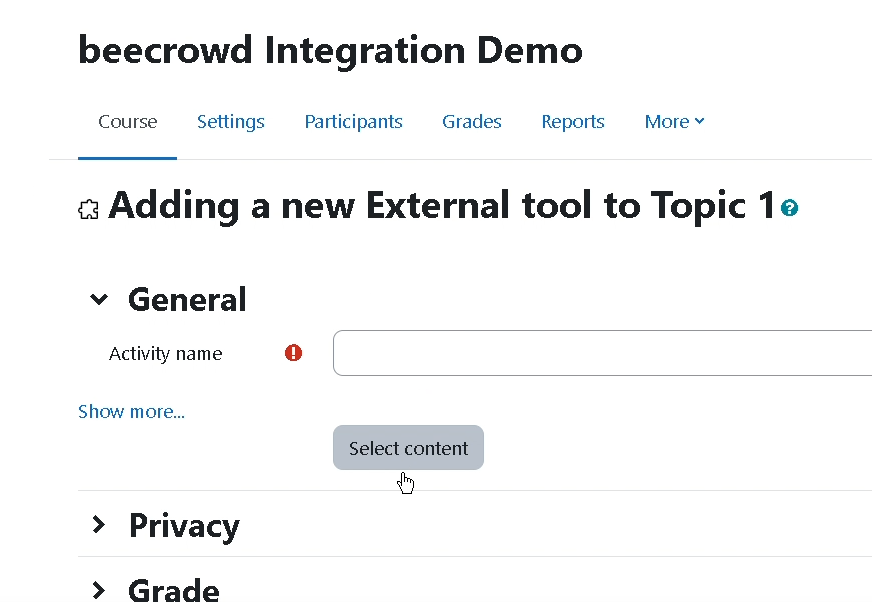
\includegraphics[scale=0.4]{pictures/apendices/apendice_b_12.png}
    \end{figure}

    \item Selecione a Disciplina criada no Beecrowd Academic:

    \begin{figure}[H]
        \centering
            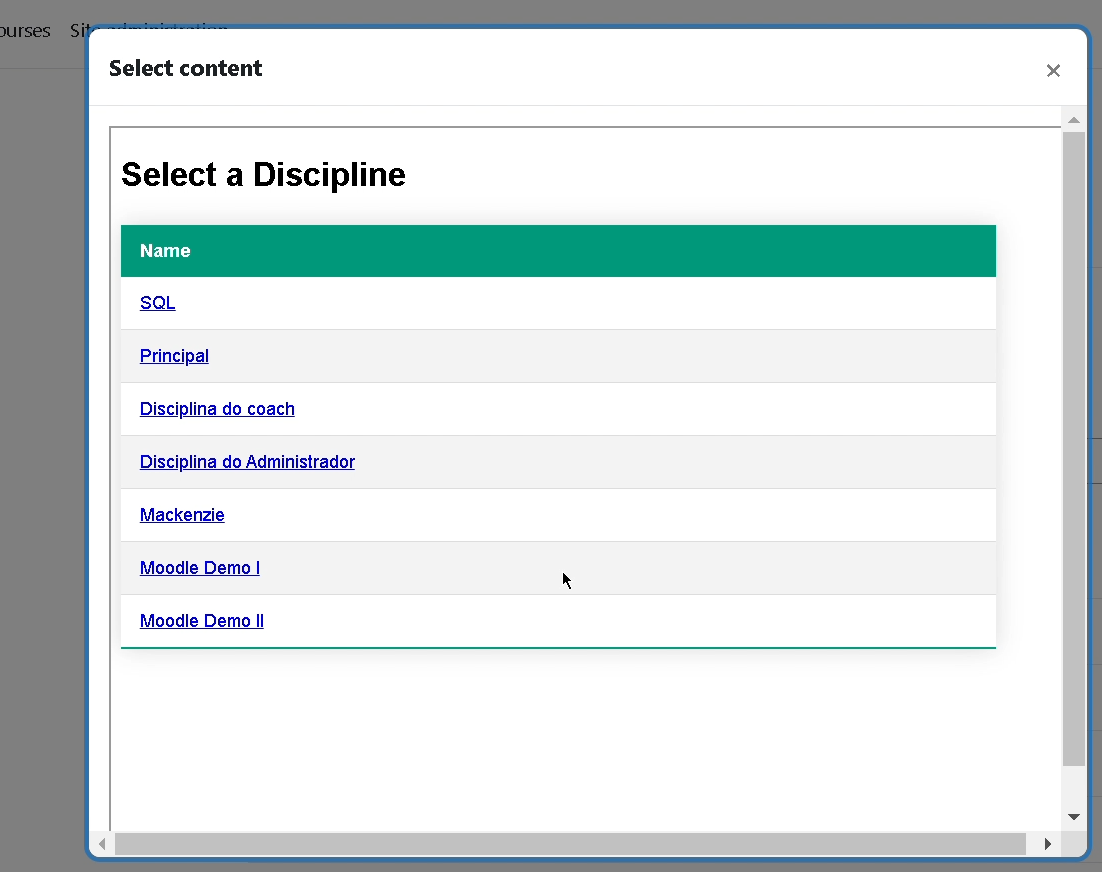
\includegraphics[scale=0.4]{pictures/apendices/apendice_b_13.png}
    \end{figure}

    \item Selecione a tarefa criada no Beecrowd Academic:

    \begin{figure}[H]
        \centering
            \includegraphics[scale=0.4]{pictures/apendices/apendice_b_14.png}
    \end{figure}

    Vai aparecer uma mensagem de confirmação que a tarefa foi selecionada com sucesso:

    \begin{figure}[H]
        \centering
            \includegraphics[scale=0.4]{pictures/apendices/apendice_b_15.png}
    \end{figure}

    \item Você vai ser redirecionado de volta para a tela anterior, e agora é só clicar em “Save and return do course”:

    \begin{figure}[H]
        \centering
            \includegraphics[scale=0.35]{pictures/apendices/apendice_b_16.png}
    \end{figure}

    Agora a tarefa aparecerá dessa forma na página do curso:

    \begin{figure}[H]
        \centering
            \includegraphics[scale=0.4]{pictures/apendices/apendice_b_17.png}
    \end{figure}
\end{enumerate}

\end{otherlanguage*}

\clearpage

\subsection{Entrando como aluno}

\begin{enumerate}
    \item O aluno clica na tarefa do Beecrowd, criada pelo professor:

    \begin{figure}[H]
        \centering
            \includegraphics[scale=0.425]{pictures/apendices/apendice_b_18.png}
    \end{figure}

    \item O aluno é direcionado à tarefa do Beecrowd, sem precisar criar um usuário, e já pode começar a resolver os exercícios da tarefa:

    \begin{figure}[H]
        \centering
            \includegraphics[scale=0.35]{pictures/apendices/apendice_b_19.png}
    \end{figure}

    Resolvendo um exercício:

    \begin{figure}[H]
        \centering
            \includegraphics[scale=0.35]{pictures/apendices/apendice_b_20.png}
    \end{figure}

    Digita o código e clica em Submit:

    \begin{figure}[H]
        \centering
            \includegraphics[scale=0.425]{pictures/apendices/apendice_b_22.png}
    \end{figure}

    O código é avaliado pelo juíz online da plataforma:

    \begin{figure}[H]
        \centering
            \includegraphics[scale=0.45]{pictures/apendices/apendice_b_23.png}
    \end{figure}
\end{enumerate}

\clearpage

\subsection{Notas}

\begin{enumerate}
    \item Após seguir os passos anteriores descritos nesse documento, o professor pode clicar na tarefa do Beecrowd que ele criou para os alunos:

    \begin{figure}[H]
        \centering
            \includegraphics[scale=0.35]{pictures/apendices/apendice_b_24.png}
    \end{figure}

    \item O professor pode visualizar quem respondeu as questões, e, ao clicar em \textbf{“Send Grades”}, as notas são enviadas para o Moodle, e o professor consegue visualizar as notas lá:

    Página da tarefa no Beecrowd Academic:

    \begin{figure}[H]
        \centering
            \includegraphics[scale=0.3]{pictures/apendices/apendice_b_25.png}
    \end{figure}

    Clica em “Send Grades”:

    \begin{figure}[H]
        \centering
            \includegraphics[scale=0.5]{pictures/apendices/apendice_b_26.png}
    \end{figure}

    Mensagem de sucesso que as notas foram enviadas:

    \begin{figure}[H]
        \centering
            \includegraphics[scale=0.43]{pictures/apendices/apendice_b_27.png}
    \end{figure}

    Notas agora estão moodle:

    \begin{figure}[H]
        \centering
            \includegraphics[scale=0.43]{pictures/apendices/apendice_b_28.png}
    \end{figure}

\end{enumerate}

\end{otherlanguage*}



        


%
% How to fix the Underfull \vbox badness has occurred while \output is active on my memoir chapter style?
% https://tex.stackexchange.com/questions/387881/how-to-fix-the-underfull-vbox-badness-has-occurred-while-output-is-active-on-m
%

% ---

\lang
% {\chapter[Page not filled]{Since this page is not being completely filled, it is generating the bottom bottom of the page}}
% {\chapter[Página não gerada]{Como esta página não está sendo completamente preenchida, ele está gerando a caixa inferior inferior da página}}
% ---


% Multiple-language document - babel - selectlanguage vs begin/end{otherlanguage}
% https://tex.stackexchange.com/questions/36526/multiple-language-document-babel-selectlanguage-vs-begin-endotherlanguage
\begin{otherlanguage*}{brazil}

\chapter{Como adicionar respostas para novas questões}
\label{manual:adicionar-respostas}

Basta adicionar um arquivo dentro do diretório \texttt{\/backend}, com o nome no formato \texttt{questao\_{numeroDaQuestao}.pl}. Cada arquivo deve seguir o seguinte padrão:

\section{Estrutura do arquivo}

\subsection{Definição do módulo}
O arquivo deve começar com a declaração do módulo. O nome do módulo deve ser igual ao nome do arquivo (sem a extensão \texttt{.pl}). Além disso, o módulo deve exportar dois predicados principais:  
\begin{itemize}
    \item \texttt{questao/3}
    \item \texttt{diagnostico/3}
\end{itemize}

Exemplo:
\begin{verbatim}
:- module(questao_2465, [questao/3, diagnostico/3]).
\end{verbatim}

\subsection{Predicado \texttt{questao/3}}
O predicado \texttt{questao/3} deve ser usado para mapear uma sequência de respostas a uma nova pergunta. Ele segue o formato:
\begin{verbatim}
questao(NumeroDaQuestao, RespostasAteAgora, Pergunta).
\end{verbatim}

\begin{itemize}
    \item \texttt{NumeroDaQuestao}: Número da questão a que o arquivo se refere.
    \item \texttt{RespostasAteAgora}: Lista de respostas fornecidas pelo usuário até o momento.
    \item \texttt{Pergunta}: Pergunta a ser exibida com base nas respostas recebidas.
\end{itemize}

Exemplo:
\begin{verbatim}
questao(2465, [], "Você quer uma dica de qual solução adotar pra esse problema?").
questao(2465, ["sim"], "Você pode usar um while True para verificar, a partir da posição (a, b) na matriz, qual vizinho...").
\end{verbatim}

\subsection{Predicado \texttt{diagnostico/3}}
O predicado \texttt{diagnostico/3} deve ser usado para fornecer um diagnóstico final ou mensagem de feedback com base nas respostas completas do usuário. Ele segue o formato:
\begin{verbatim}
diagnostico(NumeroDaQuestao, RespostasCompletas, Diagnostico).
\end{verbatim}

\begin{itemize}
    \item \texttt{NumeroDaQuestao}: Número da questão.
    \item \texttt{RespostasCompletas}: Lista de respostas fornecidas.
    \item \texttt{Diagnostico}: Diagnóstico ou feedback final.
\end{itemize}

Exemplo:
\begin{verbatim}
diagnostico(2465, ["sim", "sim", "sim"], "Legal! Parabéns!").
diagnostico(2465, _, "Atente-se bem às dicas já enviadas ou pergunte novamente!").
\end{verbatim}

\section{Considerações importantes}
\begin{itemize}
    \item Certifique-se de que todas as perguntas e diagnósticos estejam relacionados ao número da questão especificado.
    \item O sistema utilizará a lista de respostas fornecida até o momento para determinar qual pergunta exibir em seguida. Portanto, as sequências de respostas devem ser consistentes.
    \item Para mensagens genéricas ou casos em que as respostas não correspondam a nenhuma sequência específica, use \texttt{\_} como curinga no campo \texttt{RespostasCompletas} no predicado \texttt{diagnostico/3}.
\end{itemize}

Com essa estrutura, o sistema poderá processar novas questões automaticamente, bastando que o arquivo correspondente seja adicionado ao diretório.

\end{otherlanguage*}



        


%
% How to fix the Underfull \vbox badness has occurred while \output is active on my memoir chapter style?
% https://tex.stackexchange.com/questions/387881/how-to-fix-the-underfull-vbox-badness-has-occurred-while-output-is-active-on-m
%

% ---

\lang
% {\chapter[Page not filled]{Since this page is not being completely filled, it is generating the bottom bottom of the page}}
% {\chapter[Página não gerada]{Como esta página não está sendo completamente preenchida, ele está gerando a caixa inferior inferior da página}}
% ---


% Multiple-language document - babel - selectlanguage vs begin/end{otherlanguage}
% https://tex.stackexchange.com/questions/36526/multiple-language-document-babel-selectlanguage-vs-begin-endotherlanguage
\begin{otherlanguage*}{brazil}

\chapter{Artigo}

\includepdf[pages=-]{aftertext/artigo_SBC.pdf} 


\end{otherlanguage*}



        
    \end{apendicesenv}

    % Inicia os anexos
    % \begin{anexosenv}
    %     % Imprime uma página indicando o início dos anexos
    %     \ifforcedinclude\else\partanexos\fi
    %     \setlength\beforechapskip{50pt}
    %     \setlength\midchapskip{20pt}
    %     \setlength\afterchapskip{20pt}

    %     

%
% How to fix the Underfull \vbox badness has occurred while \output is active on my memoir chapter style?
% https://tex.stackexchange.com/questions/387881/how-to-fix-the-underfull-vbox-badness-has-occurred-while-output-is-active-on-m
%

% ----------------------------------------------------------
\chapter{\lang{Article published in SOBRAEP magazine}{Artigo publicado}}
% ----------------------------------------------------------


% Multiple-language document - babel - selectlanguage vs begin/end{otherlanguage}
% https://tex.stackexchange.com/questions/36526/multiple-language-document-babel-selectlanguage-vs-begin-endotherlanguage
\begin{otherlanguage*}{english}

% An environment for setting \emergencystretch locally
% https://tex.stackexchange.com/questions/84510/an-environment-for-setting-emergencystretch-locally
{
    \setlength{\emergencystretch}{10pt}
    \section[English guidelines for publication]
    {English guidelines for publication - TITLE HERE (14 PT TYPE SIZE, UPPERCASE, BOLD, CENTERED)}
}
    \noindent\textbf{Abstract:}
    The objective of this document is to instruct the authors about the preparation of the
    manuscript for its submission to the Revista Eletrônica de Potência (Brazilian Power Electronics
    Journal).~The authors should use these guidelines for preparing both the initial and final
    versions of their paper. Additional information about procedures and guidelines for publication
    can be obtained directly with the editor, or through the web site
    \url{http://www.sobraep.org.br/revista}. This text was written according to these guidelines

\end{otherlanguage*}

% What is a “Overfull \hbox (9.89561pt too wide)”?
% https://tex.stackexchange.com/questions/111948/what-is-a-overfull-hbox-9-89561pt-too-wide
interwordspace: \the\fontdimen2\font

interwordstretch: \the\fontdimen3\font

emergencystretch: \the\emergencystretch\par\relax


\modifiedincludepdf{-}{ArtigoSOBRAEP}{pictures/SOBRAEP.pdf}{0.9}



    %     


%
% How to fix the Underfull \vbox badness has occurred while \output is active on my memoir chapter style?
% https://tex.stackexchange.com/questions/387881/how-to-fix-the-underfull-vbox-badness-has-occurred-while-output-is-active-on-m
%

% ----------------------------------------------------------
\lang
{\chapter[Sample example]{How to display the font size in use in the final output}}
{\chapter[Anexo exemplo]{Como exibir o tamanho da fonte em uso na saída final}}
% ----------------------------------------------------------


% Multiple-language document - babel - selectlanguage vs begin/end{otherlanguage}
% https://tex.stackexchange.com/questions/36526/multiple-language-document-babel-selectlanguage-vs-begin-endotherlanguage
\begin{otherlanguage*}{english}

\showfont

1. How to display the font size in use in the final output,
2. How to display the font size in use in the final output,
3. How to display the font size in use in the final output,


\section[Some encoding tests]{\showfont}

1. How to display the font size in use in the final output,
2. How to display the font size in use in the final output,
3. How to display the font size in use in the final output,
4. How to display the font size in use in the final output,
5. How to display the font size in use in the final output,
6. How to display the font size in use in the final output,

7. How to display the font size in use in the final output,
8. How to display the font size in use in the final output,
9. How to display the font size in use in the final output,
10. How to display the font size in use in the final output,
11. How to display the font size in use in the final output,
12. How to display the font size in use in the final output,

\subsection{\showfont}

1. How to display the font size in use in the final output,
2. How to display the font size in use in the final output,
3. How to display the font size in use in the final output,
4. How to display the font size in use in the final output,
5. How to display the font size in use in the final output,
6. How to display the font size in use in the final output,

7. How to display the font size in use in the final output,
8. How to display the font size in use in the final output,
9. How to display the font size in use in the final output,
10. How to display the font size in use in the final output,
11. How to display the font size in use in the final output,
12. How to display the font size in use in the final output,

\subsubsection{\showfont}

1. How to display the font size in use in the final output,
2. How to display the font size in use in the final output,
3. How to display the font size in use in the final output,
4. How to display the font size in use in the final output,
5. How to display the font size in use in the final output,
6. How to display the font size in use in the final output,

7. How to display the font size in use in the final output,
8. How to display the font size in use in the final output,
9. How to display the font size in use in the final output,
10. How to display the font size in use in the final output,
11. How to display the font size in use in the final output,
12. How to display the font size in use in the final output,

\subsubsubsection{\showfont}

1. How to display the font size in use in the final output,
2. How to display the font size in use in the final output,
3. How to display the font size in use in the final output,
4. How to display the font size in use in the final output,
5. How to display the font size in use in the final output,
6. How to display the font size in use in the final output,
7. How to display the font size in use in the final output,

8. How to display the font size in use in the final output,
9. How to display the font size in use in the final output,
10. How to display the font size in use in the final output,
11. How to display the font size in use in the final output,
12. How to display the font size in use in the final output,


Lipsum me [55-65]

\end{otherlanguage*}



    % \end{anexosenv}

    % INDICE REMISSIVO
    \ifforcedinclude\else
        \phantompart
        \printindex
    \fi

\end{document}

